\documentclass{article}

% Language setting
\usepackage[english]{babel}

% Set page size and margins
\usepackage[a4paper,top=2cm,bottom=2cm,left=3cm,right=3cm,marginparwidth=1.75cm]{geometry}

% Useful packages
\usepackage{pgfplots}
\usepackage{callouts-box}
\usepackage{stix}
\usepackage{amsmath}
\usepackage{circuitikz}
\usepackage{graphicx}
\usepackage[utf8]{inputenc}
\usepackage[colorlinks=true,linkcolor=black,urlcolor=blue,citecolor=blue,filecolor=blue]{hyperref}
\usepackage[all]{hypcap} % Load this *after* hyperref
\usepackage{listings}
\usepackage{xcolor}
\usepackage{titlesec}
\usepackage{placeins}

\titleformat{\section}
    {\normalfont\huge\bfseries}
    {\thesection}{1em}{}

\pgfplotsset{width=10cm,compat=1.9}

\definecolor{backcolour}{rgb}{0.97,0.97,0.95}
\definecolor{keywordcolor}{rgb}{0.86,0.12,0.34}
\definecolor{commentcolor}{rgb}{0.34,0.54,0.32}
\definecolor{stringcolor}{rgb}{0.76,0.38,0.11}
\definecolor{identifiercolor}{rgb}{0.20,0.20,0.7}
\definecolor{linenumbergray}{gray}{0.4}

\lstset{
    backgroundcolor=\color{backcolour},   
    basicstyle=\ttfamily\small,
    commentstyle=\color{commentcolor}\itshape,
    keywordstyle=\color{keywordcolor}\bfseries,
    stringstyle=\color{stringcolor},
    showstringspaces=false,
    breaklines=true,
    frame=single,
    numbers=left,
    numberstyle=\tiny\color{linenumbergray},
    tabsize=2,
    captionpos=b,
    literate={~}{{\raisebox{0.6ex}{\texttildelow}}}{1}
}

\lstdefinelanguage{sdc}{
    keywords={create_clock, create_generated_clock, set_input_delay, set_output_delay, set_false_path, set_max_delay}, 
    comment=[l]{\#}   
}

\begin{document}
    
    \begin{titlepage}
        
        \centering
        
        \vspace*{2cm}
        
        
\includegraphics[width=0.3\linewidth]{img/Stemma_unipi.jpg}
        
        {\LARGE \textbf{University of Pisa}\\[1em]}
        {\Large Department of Information Engineering\\[1em]}
        {\large Master’s Degree in Electronic Engineering\\}
        {\large Microelectronic System Design\\[3em]}
        {\huge \textbf{Design of a function generator using CycloneII FPGA}\\[1em]}
        {\large Academic Year 2025/2026}
        
        \vfill
        
        \begin{flushleft}
            \textbf{Students:}\\
            Dario Aliberti\\
            Tommaso Tonarini
        \end{flushleft}
        
        \vspace{1cm}
        
    \end{titlepage}
    
    \newpage
    \tableofcontents
    
    
    \newpage
    \section{Introduction}
\label{sec:introduction}

Frequency generators are electronic devices widely used in laboratories to generate electrical waves with the desired shapes. The most common waveforms used are sinusoidal, triangular, and square, but sometimes sinc, noise, and other less common waves are also used.
To generate an analog waveform with a digital circuit, different techniques are used, but each one is made of these blocks

\begin{itemize}
        
    \item \textbf{Human-Machine interface} \newline
    It is used to choose the waveform to be generated

    \item \textbf{Digital waveform generator} \newline
    It is the digital block that sends data to be converted into analog signals with the right timing specifications

    \item \textbf{Digital analog converter} \newline
    It is the component that converts the digital signals into analog signals
        
\end{itemize}

\noindent
The main blocks used to implement the function generator will now be briefly described.

\subsection{DDFS tecnique}

The DDFS tecnique also called \textbf{Direct Digital Frequency synthesis} is a type of digital electronic signal generator that read the data stored in a memory called LUT or \textbf{Look Up Table} to generate the samples for the desired signal.
\begin{center}
    \vspace*{1cm}
    \scalebox{0.79}{
        \begin{tikzpicture}
            \tikzset{one bit adder/.style={muxdemux,
                muxdemux def={Lh=4, NL=2, Rh=2, NR=1, NB=1, w=2.5,
                inset w=0.5, inset Lh=2, inset Rh=1.5}}}
                        
            \node[one bit adder, fill=cyan!30!white] (fa) at (6.53, 4) {\Large $\oplus$};
            \node[flipflop D, xscale=0.7, yscale=0.7, fill=cyan!30!white] at (9.784, 3.412){};
            \draw (7.5, 4) to[multiwire] (9, 4);
            \draw (10.568, 4) -| (11, 4) -| (11, 6.5) to[multiwire] (4.75, 6.5) -- (4.75, 4.84) -| (5.55, 4.84);
            \draw (5.55, 3.161) to[multiwire] (3, 3.161);
            \draw (9, 2.824) -| (8, 2) to[multiwire] (3, 2);
            \node[shape=rectangle, draw, line width=1pt, minimum width=1.965cm, minimum height=3.215cm, fill=cyan!30!white](N1) at (13, 4){} node[anchor=center] at (N1.text){$LUT$};
            \draw (11, 4) to[multiwire] (12, 4);
            \node[shape=rectangle, minimum width=0.8cm, minimum height=0.465cm] 
            at (2.625, 3.75) {};
        
            \node[
                shape=rectangle,
                minimum width=0.8cm,
                minimum height=0.465cm,
                align=center
            ] at (2.625, 3.2) {fw};
    
            \node[
                shape=rectangle,
                minimum width=0.8cm,
                minimum height=0.465cm,
                align=center
            ] at (2.625, 2.05) {clk};
        
        \end{tikzpicture}
    }
    \vspace*{1cm}        
\end{center}

\noindent
The DDFS signal generator is based on a counter called \textbf{phase accumulator}. \newline
The output of this counter is increased, at every positive edge of the clock signal, by the value stored in the variable \(f_w\), called \textbf{frequency word}. \newline
Then, the output of the counter is used as the address for a Look-Up Table memory that contains the samples of the signal to be generated.

\newpage

\subsubsection{Amplitude quantization}
The digital output value from the LUT is sent to an external \textbf{digital to analog converter}, and the number of bits used to store each sample of the wave determines the smallest amplitude swing that the wave can produce.\\
If we use a \textbf{C2 balanced representation} to generate the wave, the smallest output voltage swing is

\vspace*{0.25cm} 
\[
    min( \Delta V_{out} ) = \frac{V_{cc}}{2^N - 1}
\]
\vspace*{0.25cm} 

\noindent
where \(N\) is the number of bits for the signal samples and \(V_{cc}\) is the maximum output voltage of the DAC.

\subsubsection{Frequency quantization}
The samples are sent to the DAC at the clock frequency; indeed, at every positive edge of the clock, the flip-flop updates the output and the adder increases the input of the register for the next address value.  \\
The address does not increase by a unit amount, but depends on the value of \(f_w\); with this procedure, we can control the frequency of the output wave simply by adjusting the value of \(f_w\). \\
The output frequency of the wave is

\vspace*{0.25cm} 
\[
    f = f_{clk} \cdot \frac{f_{w}}{\texttt{LUT\_DIM}}
\]
\vspace*{0.25cm} 

\noindent
where \(f_{clk}\) is the clock frequency of the DDFS and \(LUT\_DIM\) is the number of samples stored in the LUT.
The problem is that increasing the value of \(f_w\) involves an increase in the output wave frequency, but a reduction in the number of samples used for the generation of the wave, which results in a stepped output signal.

\newpage

\subsubsection{LUT optimization}
Some types of waves have a quadrangular-symmetrical profile, meaning a periodic signal that, every quarter of its period, is reproduced by a vertical symmetry, and every half of its period by a horizontal symmetry.

\begin{center}

    \vspace*{0.5cm}
    \scalebox{0.9}{
        \begin{minipage}{0.45\textwidth}
            \begin{tikzpicture}[scale=0.7]
                \begin{axis}[
                    axis lines = middle,
                    xlabel = {$t$},
                    ylabel = {$f(t)$},
                    xmin = 0, xmax = 2*pi+0.5,
                    ymin = -1.8, ymax = 1.1,
                    samples = 200,
                    xtick = {pi/2, pi, 3*pi/2, 2*pi},
                    xticklabels = {$\frac{1}{4f_o}$, $\frac{1}{2f_o}$, $\frac{3}{4f_o}$, $\frac{1}{f_o}$},
                    ytick = {-1, 0, 1},
                    yticklabels = {$f_{min}$, 0, $f_{max}$}
                ]
                
                \addplot [red, thick, domain=0:2*pi] {sin(deg(x))^3};
                
                \draw[dashed] (axis cs:2*pi, -1.7) -- (axis cs:2*pi, -0.33);
                \draw[dashed] (axis cs:pi, -1.5) -- (axis cs:pi, -0.33);
                \draw[dashed] (axis cs:pi/2, -1.3) -- (axis cs:pi/2, -0.33);
                \draw[dashed] (axis cs:3*pi/2, -1.3) -- (axis cs:3*pi/2, -0.33);
                
                \draw[<->] (axis cs:0, -1.6) -- node[below] {$T$} (axis cs:2*pi, -1.6);
                \draw[<->] (axis cs:0, -1.4) -- node[below] {$T/2$} (axis cs:pi, -1.4);
                \draw[<->] (axis cs:pi, -1.4) -- node[below] {$T/2$} (axis cs:2*pi, -1.4);
                \draw[<->] (axis cs:0, -1.2) -- node[below] {$T/4$} (axis cs:pi/2, -1.2);
                \draw[<->] (axis cs:pi/2, -1.2) -- node[below] {$T/4$} (axis cs:pi, -1.2);
                \draw[<->] (axis cs:pi, -1.2) -- node[below] {$T/4$} (axis cs:3*pi/2, -1.2);
                \draw[<->] (axis cs:3*pi/2, -1.2) -- node[below] {$T/4$} (axis cs:2*pi, -1.2);
                
                \end{axis}
                
            \end{tikzpicture}
        \end{minipage}
        \hfill
        \begin{minipage}{0.45\textwidth}
            \scalebox{0.9}{
                \parbox{\linewidth}{
                    \textbf{Vertical symmetry:}
                    \[
                        \begin{aligned}
                            f\Bigl(\frac{T}{4}+t\Bigr) &= f\Bigl(\frac{T}{4}-t\Bigr) \quad t \in [0,T/2] \\
                            f\Bigl(\frac{3T}{4}+t\Bigr) &= f\Bigl(\frac{3T}{4}-t\Bigr) \quad t \in [T/2,T]
                        \end{aligned}
                    \]
                    
                    \textbf{Horizontal symmetry:}
                    \[
                        \begin{aligned}
                            f\Bigl(\frac{T}{2}+t\Bigr) &= -f\Bigl(\frac{T}{2}-t\Bigr) \quad t \in [0,T]
                        \end{aligned}
                    \]
                }
            }
        \end{minipage}
    }
    \vspace*{0.5cm} 

\end{center}

\noindent
For this type of wave, it is sufficient to store a quarter of the full period, and by reading the value of the phase accumulator, it can be determined whether vertical symmetry or horizontal symmetry needs to be applied.  \\
With this technique the dimension of the LUT can be reduced by a factor of 4. \\
To apply vertical symmetry, the LUT must be read from bottom to top, and to apply horizontal symmetry, the output signal must be inverted by changing its sign.  \\
Vertical symmetry should be applied during the second and fourth quarters of the period, while horizontal symmetry should be applied during the second half of the period. Therefore, if the LUT size is a power of two, the vertical symmetry signal can be \(y(MSB-1)\) and the horizontal symmetry signal \(y(MSB)\), where \(y(n)\) is the n-th output bit of the phase accumulator.
Using a C2 representation the \textbf{LUT optimization circuit} can be done as follows

\begin{center}
    \vspace*{1cm}
    \scalebox{0.79}{
        \begin{tikzpicture}
            \tikzset{one bit adder/.style={muxdemux,
                muxdemux def={Lh=4, NL=2, Rh=2, NR=1, NB=1, w=2.5,
                inset w=0.5, inset Lh=2, inset Rh=1.5}}}
            \tikzset{mux/.style={muxdemux,
                muxdemux def={Lh=4, NL=2, Rh=3,
                NB=1, w=2, square pins=1}}}
                        
            \node[one bit adder, fill=cyan!30!white] at (6.53, 4) {\Large $\oplus$};
            \node [mux, fill=red!30!white] (mux1) at (4, 3.16){MUX};
            \node [mux, fill=red!30!white] (mux2) at (18, 3.45){MUX};
            \node[flipflop D, xscale=0.7, yscale=0.7, fill=cyan!30!white] at (9.784, 3.412){};
            \draw (7.5, 4) to[multiwire] (9, 4);
            \draw (10.568, 4) -| (11, 4) -| (11, 6.5) to[multiwire] (4.75, 6.5) -- (4.75, 4.84) -| (5.55, 4.84);
            \draw (5.55, 3.161) to[multiwire] (4.835, 3.161);
            \draw (9, 2.824) -| (8, 0) -- (1, 0);
            \node[shape=rectangle, draw, line width=1pt, minimum width=1.965cm, minimum height=3.215cm, fill=cyan!30!white](N1) at (13, 4){} node[anchor=center] at (N1.text){$LUT$};
            \draw (11, 4) to[multiwire] (12, 4);
            \node[shape=rectangle, minimum width=0.8cm, minimum height=0.465cm] 
            at (2.625, 3.75) {};
            
            \node[ieeestd not port, rotate=0, scale=0.4, fill=red!30!white] (not1) at ($(mux1.lpin 2)+(-0.5,0)$) {};
            \node[ieeestd not port, rotate=0, scale=0.4, fill=red!30!white] (not2) at ($(mux2.lpin 2)+(-0.5,0)$) {};
            
            \node[
                shape=rectangle,
                minimum width=0.8cm,
                minimum height=0.465cm,
                align=center
            ] (fw) at ($(mux1.lpin 1) + (-2.5,0)$) {fw};

             \node[
                shape=rectangle,
                minimum width=0.8cm,
                minimum height=0.465cm,
                align=center
            ] (y1) at ($(mux1.bpin 1) + (0,-0.7)$) {y(MSB-1)};

            \draw (mux1.bpin 1) -- ($(mux1.bpin 1) + (0,-0.4)$);

            \node[
                shape=rectangle,
                minimum width=0.8cm,
                minimum height=0.465cm,
                align=center
            ] (y2) at ($(mux2.bpin 1) + (0,-0.7)$) {y(MSB)};
            
            \node[
                shape=rectangle,
                minimum width=0.8cm,
                minimum height=0.465cm,
                align=center
            ] (y2) at (9.85, 6.8) {y(MSB-2 .. 0)};

            \draw (mux2.bpin 1) -- ($(mux2.bpin 1) + (0,-0.4)$);
            
            \draw ($(mux1.lpin 1) + (-2.2,0)$) to[multiwire] (mux1.lpin 1);
            \draw (not1.in) -| ($(mux1.lpin 1) + (-1.7,0)$);
            \draw (not2.in) -| ($(mux2.lpin 1) + (-1.7,0)$);

            \draw (not1.out) -- (mux1.lpin 2);
            \draw (not2.out) -- (mux2.lpin 2);

            \draw (14, 4) to[multiwire] (15.5, 4);
            \draw (15.5, 4) to[multiwire] (mux2.lpin 1);
    
            \node[
                shape=rectangle,
                minimum width=0.8cm,
                minimum height=0.465cm,
                align=center
            ] at (0.65, 0.05) {clk};
        
        \end{tikzpicture}
    }
    \vspace*{1cm}
    
\end{center}


\newpage

\subsection{Parallel bus DAC}

The DAC, or \textbf{digital to analog converter}, is a device that takes a digital value as input and provides an analog output signal proportional to it. \\
The output voltage of the DAC can be calculated with the following formula


\vspace*{0.25cm} 
\[
    V_{out} = \frac{n}{2^N-1} \cdot V_{max}
\]
\vspace*{0.25cm} 

\noindent
where \(N\) is the number of digital input bits, \(n\) is the input value of the DAC, and \(V_{max}\) is the maximum output voltage of the DAC. \\
For the most common types of DACs, the input signal is expressed as an unsigned value represented in C1 notation.

\subsubsection{R-2R ladder DAC}
One of the most common types of DAC is the R–2R ladder, where the output voltage depends on the input voltage values \(V_0 \ldots V_N\). \\
The output of the ladder is usually buffered with an operational amplifier to ensure that the output resistance seen from the ladder is always high, independently of the value of the load resistance.

\begin{center}

    \vspace*{0.5cm}
    \scalebox{0.7}{
        \begin{tikzpicture}
            \node[op amp] at (11.19, 5.49){};
            \draw (7, 5) to[american resistor, l={$R$}] (8.75, 5);
            \draw (6.5, 4.5) to[american resistor, l={$2R$}] (6.5, 2.75);
            \draw (4.25, 5) to[american resistor, l={$R$}] (6, 5);
            \draw (3.75, 4.5) to[american resistor, l={$2R$}] (3.75, 2.75);
            \draw (1.5, 5) to[american resistor, l={$R$}] (3.25, 5);
            \draw (1, 4.5) to[american resistor, l={$2R$}] (1, 2.75);
            \draw (9.25, 4.5) to[american resistor, l={$2R$}] (9.25, 2.75);
            \draw (-1, 4.5) to[american resistor, l={$2R$}] (-1, 2.75);
            \draw (6, 5) -- (7, 5);
            \draw (6.5, 4.5) -| (6.5, 5);
            \draw (3.25, 5) -- (4.25, 5);
            \draw (3.75, 4.5) -| (3.75, 5);
            \draw (-1, 4.5) -| (-1, 5) -- (1.5, 5);
            \draw (1, 4.5) -| (1, 5);
            \draw (8.75, 5) -- (10, 5);
            \draw (9.25, 4.5) -| (9.25, 5);
            \draw (10, 5.98) -| (9.5, 6) |- (13, 7.25) -| (13, 5.5) |- (12.38, 5.49);
            \node[circ] at (3.75, 5){};
            \node[circ] at (1, 5){};
            \node[circ] at (6.5, 5){};
            \node[circ] at (9.25, 5){};
            \node[cground] at (-1, 2.75){};
            \node[shape=rectangle, minimum width=0.715cm, minimum height=0.715cm](N1) at (1, 2.375){} node[anchor=center] at (N1.text){$V_0$} node[anchor=north, align=center, text width=0.327cm, inner sep=6pt] at (1, 2.75){};
            \node[shape=rectangle, minimum width=0.715cm, minimum height=0.715cm](N2) at (3.75, 2.375){} node[anchor=center] at (N2.text){$V_1$} node[anchor=north, align=center, text width=0.327cm, inner sep=6pt] at (3.75, 2.75){};
            \node[shape=rectangle, minimum width=0.715cm, minimum height=0.715cm](N3) at (6.5, 2.375){} node[anchor=center] at (N3.text){$V_2$} node[anchor=north, align=center, text width=0.327cm, inner sep=6pt] at (6.5, 2.75){};
            \node[shape=rectangle, minimum width=0.715cm, minimum height=0.715cm](N4) at (9.25, 2.375){} node[anchor=center] at (N4.text){$V_3$} node[anchor=north, align=center, text width=0.327cm, inner sep=6pt] at (9.25, 2.75){};
            \node[shape=rectangle, minimum width=0.715cm, minimum height=0.715cm](N5) at (13.5, 5.5){} node[anchor=center] at (N5.text){$V_{out}$} node[anchor=north, align=center, text width=0.327cm, inner sep=6pt] at (13.5, 5.875){};
        \end{tikzpicture}
    }

    \vspace*{0.5cm}
    
\end{center}

\noindent
The output voltage for this type of DAC can be calculated as follows

\vspace*{0.25cm}
\[
    V_{out}[4 \ bit] = \frac{2^0 \cdot V_0 + 2^1 \cdot V_1 + 2^2 \cdot V_2 + 2^3 \cdot V_3}{2^4} \implies
    V_{out}[n \ bit] = \frac{1}{2^N} \cdot \sum_{i=0}^{N-1} {(2^i \cdot V_i)}
\]
\vspace*{0.25cm}

\noindent
where the first formula refers to a 4-bit R-2R ladder DAC (as shown in the image above), and the second formula refers to a generic N-bit DAC. \\
The most critical aspect of using this type of DAC is that the output voltage error is proportional to the mismatch of the resistor values and that the voltage across the resistors dissipates power. \\
For this reasons, they are not recommended for low-power or high-precision applications.

        
\newpage

\subsection{Button matrix keypad}

The \textbf{button matrix keypad} is a device used to interface an electrical device with the user. \\
The device is composed of multiple buttons, and usually, to reduce the number of connection pins, the buttons are connected in a matrix, as shown in the figure below.

\vspace*{0.25cm}
\begin{center}
    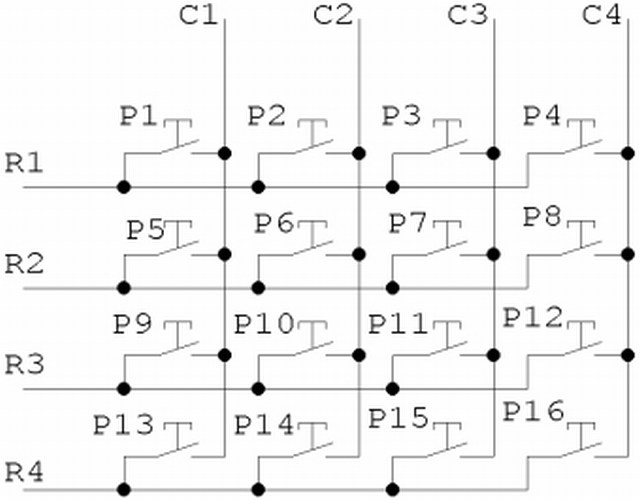
\includegraphics[width=0.35\linewidth]{img/pic_schema_tastiera.jpg}
\end{center}
\vspace*{0.25cm}

\noindent
To read the button pressed the rows must be connected to \(0V\) or \(V_{cc}\) and the column have to be read following this sequence:

\begin{itemize}

    \item \(R1 = V_{cc} \quad R2 = 0V \quad R3 = 0V \quad R4 = 0V\) \\
    the first row is enabled and the others are disabled, so the \(C_1 \quad ... \quad C4\) read values are referred to \(P1 \quad ...\quad P4\)

    \item \(R1 = 0V \quad R2 = V_{cc} \quad R3 = 0V \quad R4 = 0V\) \\
    the second row is enabled and the others are disabled, so the \(C_1 \quad ... \quad C4\) read values are referred to \(P5 \quad ...\quad P6\)
    
    \item \(R1 = 0V \quad R2 = 0V \quad R3 = V_{cc} \quad R4 = 0V\) \\
    the third row is enabled and the others are disabled, so the \(C_1 \quad ... \quad C4\) read values are referred to \(P9 \quad ...\quad P10\)
    
    \item \(R1 = 0V \quad R2 = 0V \quad R3 = 0V \quad R4 = V_{cc}\) \\
    the fourth row is enabled and the others are disabled, so the \(C_1 \quad ... \quad C4\) read values are referred to \(P13 \quad ...\quad P16\)
\end{itemize}

\noindent
Thus, the principle is to enable the row containing the pressed button and read the corresponding column wire. \\
The entire enable sequence (from enabling the first row to enabling the last row) must be completed faster than the user's response time. \\
This is usually not a problem, because a person has a response time greater than \(100 \, \mathrm{ms}\); therefore, with a scanning frequency greater than \(40 \, \mathrm{Hz} \simeq \text{row\_number}/100\,\mathrm{ms}\), the user does not perceive any delay when pressing the button.
To read the keypad, the rows must be enabled sequentially. \\
However, if two buttons in the same column are pressed at the same time, the rows can become shorted, which may be dangerous for the system. \\
For this reason, diodes are used when connecting the rows. \\
The columns are floating when no button is pressed, so pull-down (or pull-up, depending on the keypad reading logic) resistors are required.


\newpage

\subsection{LCD communication}

We use the \textbf{16x2 LCD Module} (\texttt{CFAH1602B-TMC-JP}) integrated in the \textbf{Altera DE2 board} to show the selected wave function name and wave frequency. \\
The LCD Module has built in a LSI controller, the controller has two 8-bit registers, an \textbf{instruction register} (IR) and a \textbf{data register} (DR). \\
The IR stores instruction codes, such as display clear and cursor shift, and address information for display data RAM (DDRAM). \\
These two registers can be selected with the \textbf{register selector} (RS) signal, if it is set to low is possible to write an operation into the IR register, else if the RS signal is set to high the data are written from the DR to the DDRAM. \\
The R/W pin can be used to read the Busy Flag (BF), if is enabled, or to read data from DDRAM or CGRAM. \\
Since we don't need those functions we leave it always low.

\vspace{0.5cm}
\begin{figure}[h!]
    \centering
    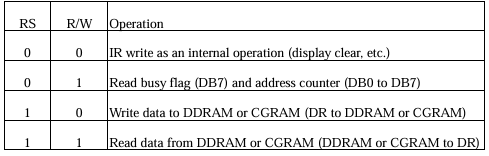
\includegraphics[width=0.6\linewidth]{img/LCD_rs_rw_table.png}
    \caption{Operation selection}
    \label{fig:LCD_rs_rw_table}
\end{figure}
\vspace{0.5cm}

\subsubsection{Character display}
An internal Address Counter (AC) is used to increment the DDRAM address each new writing cycle. \\
The Character Generator ROM (CGROM) generates 5x8 dot or 5x10 dot character patters from 8 bit ASCII code stored in the DDRAM to be displayed on the screen. \\
The table \autoref{fig:LCD_character_generator} shows how CGROM can output a unique set of dots for each character. 

\vspace{0.5cm}
\begin{figure}[h!]
    \centering
    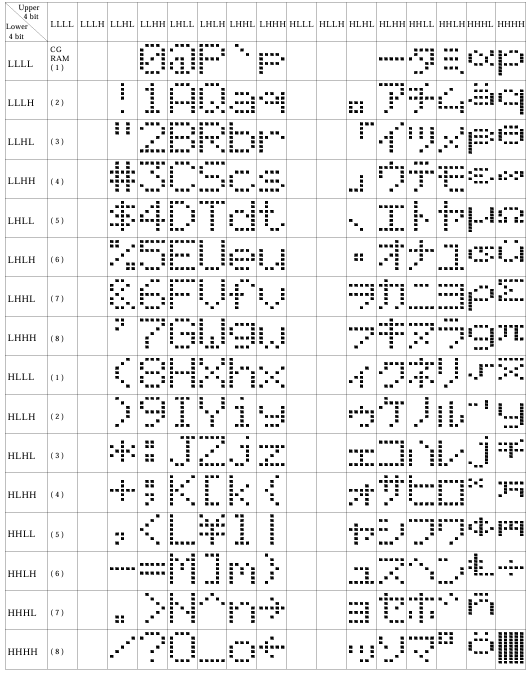
\includegraphics[width=0.45\linewidth]{img/LCD_character_generator.png}
    \caption{Character Generator ROM pattern}
    \label{fig:LCD_character_generator}
\end{figure}
\vspace{0.5cm}

\subsubsection{Timing Characteristics}
It is essential to respect the timing characteristic of LCD module to correctly complete a write cycle without issues. \\
As we can see in \autoref{fig:LCD_write_cycle} the RS and R/W signals need to be stable before the E signal is set to high and the enable pulse needs to be sufficiently wide to collect the data, then after disabling E an hold time is required to complete the cycle. \\
In our case a fast display refresh frequency is not required, so it is possible to use delays way larger than the stated times reported by the datasheet, nonetheless the correct sequence of the chip enable (E) needs to be used.

\vspace{0.5cm}
\begin{figure}[h!]
    \centering
    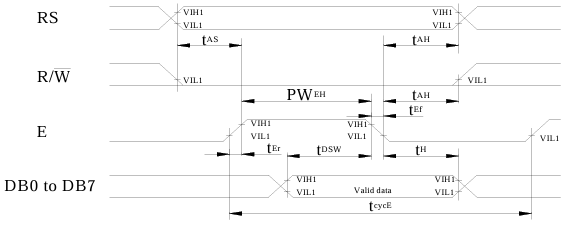
\includegraphics[width=0.8\linewidth]{img/LCD_write_cycle.png}
    \caption{Write Operation}
    \label{fig:LCD_write_cycle}
\end{figure}
\vspace{0.5cm}
    
    \newpage
    \section{Description of the architecture}
\label{sec:description_of_the_architecture}

To analyze the frequency generator designed for this project, we can start from the structure of three main blocks

\begin{itemize}
        
    \item \textbf{Human-Machine interface} \newline
    To select the desired output wave at the right frequency, this generator provides an LCD screen and a keypad. \\
    The keypad is used to write the frequency manually and to select the output waveform, information that is shown on the LCD screen.

    \item \textbf{Digital waveform generator} \newline
    The digital waveform generator uses the DDFS technique to create the digital output. \\
    The representation of the output value is C1 to be compatible with the DAC, and to increase the number of waveforms available, vertical and horizontal mirroring is selectable.

    \item \textbf{Digital analog converter} \newline
    The DDFS module is designed to have a \(12 \ bit\) output digital value, but for the project a is used a VGA DAC that has three \(10 \ bit\) channels. \\
    Only the most significant bits of the module have been used.

        
\end{itemize}

\subsection{Specifications}

The frequency generator designed is capable to generate three different output wave and the mirroring combinations of them, with a total of 8 valid combinations (some combinations are valid but not useful)

\begin{itemize}

    \item \textbf{Square wave} \\
    available only with vertical and horizontal mirroring enabled, for every other combinations of vertical and horizontal mirroring the output value is constant at \texttt{0xFFF} (hex notation), or result in a square wave with two time the selected frequency.
    
    \item \textbf{Triangular wave} \\
    available with vertical and horizontal mirroring enabled.
    If the vertical and the horizontal mirroring is disabled the output is a \textbf{sawtooth wave},
    instead if only the horizontal mirroring is enabled, the output is an \textbf{alternating symmetrical sawtooth wave}
    
    \item \textbf{Sinusoidal wave} \\
    available with vertical and horizontal mirroring enabled.
    If only the vertical mirroring is enabled the waveform is a \textbf{rectified sinusoidal wave}.
    If only the horizontal mirroring is enabled the waveform is an \textbf{alternating symmetrical quarter-sine wave}.
    If both of the mirroring are disabled the waveform is a \textbf{quarter-sine wave}
    
\end{itemize}

\noindent
The output frequency can be selected with an LCD screen and a keypad and can go from \(1Hz\) to \(1MHz\) without using external memory for the LUT.

\vspace{0.5cm}
\[
    max(f_{out}) = \frac{max(f_{clk})}{\texttt{LUT\_DIM}/max(f_w) \cdot 4} = \frac{35MHz}{2^{10}/2^7 \cdot 4} \simeq 1.09MHz
\]
\vspace{0.5cm}

\noindent
The DAC used is a \(10 \ bit\) VGA DAC with three channels synchronized with a common clock at the maximum frequency of \(100 \ MHz\). \\
The maximum clock frequency is \(35MHz\) because the project is synchronized with a common clock source at a frequency of \(70MHz\) that passes through a frequency divider, which dynamically divides the frequency with a division coefficient ranging from \(2\) to \(1000000\).

\newpage

\subsection{Module description}

As seen in the image below, the project is made of different modules 

\begin{figure}[h!]
    \centering
    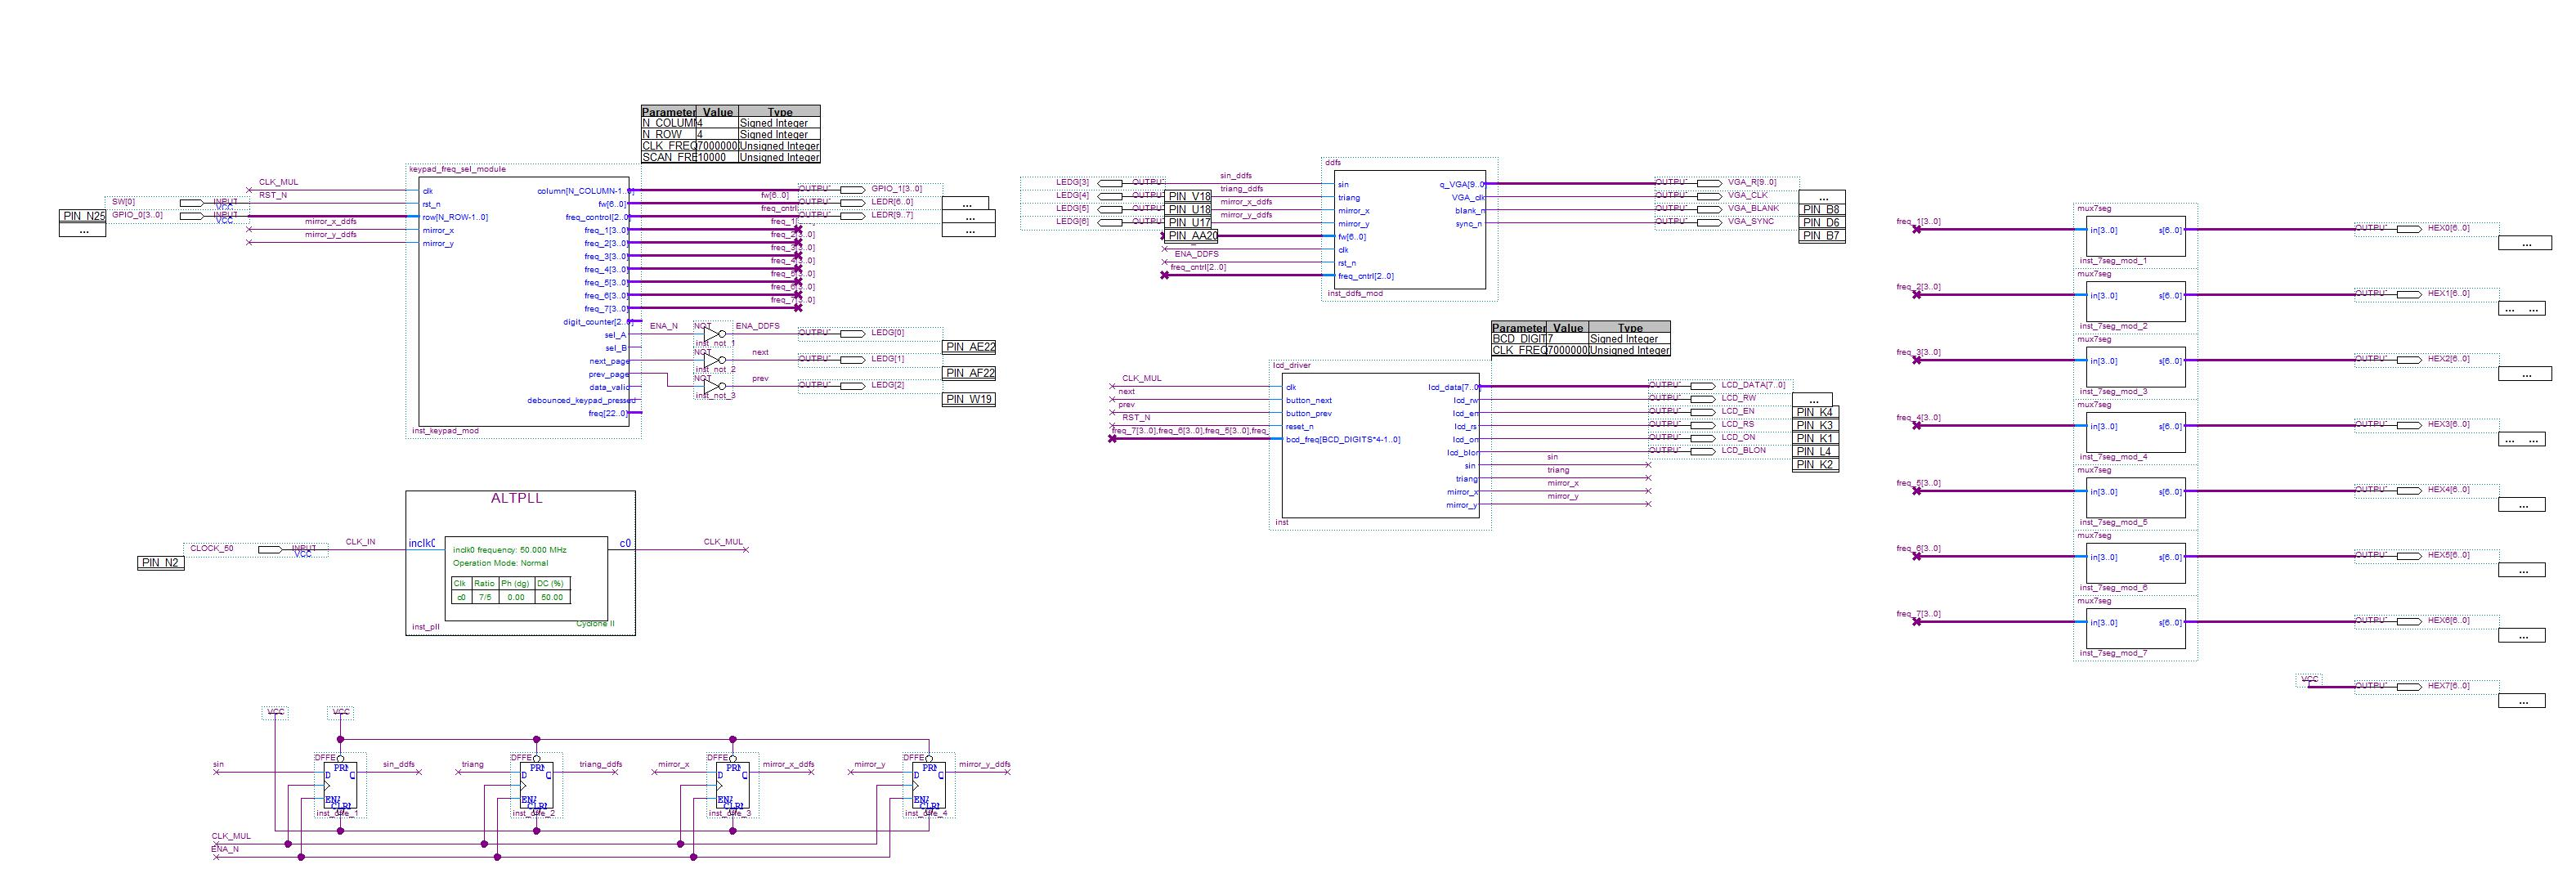
\includegraphics[width=\textwidth]{img/main_function_generator.jpg}
    \caption{Top level entity symbol schematic}
    \label{fig:Top_level_entity}
\end{figure}

\subsubsection{DDFS module}

The DDFS module generates the bit-stream corresponding to the samples of the output waveform at the desired frequency. \\
The samples are synchronized with a common clock signal, and the frequency of the output wave can be selected through the \texttt{fw} and \texttt{freq\_ctrl} inputs. \\
This module has been designed in two different ways:

\begin{itemize}
    \item the first version is intended to be connected to the \textbf{ADV7123 DAC}, which is a \(10 bit\) synchronous VGA DAC
    \item the second version is intended to be connected to a \(12 bit\) asynchronous R-2R ladder DAC.
\end{itemize}

\vspace*{0.5cm}
\begin{figure}[h!]
    \centering
    % Immagine a sinistra
    \begin{minipage}{0.45\textwidth}
        \centering
        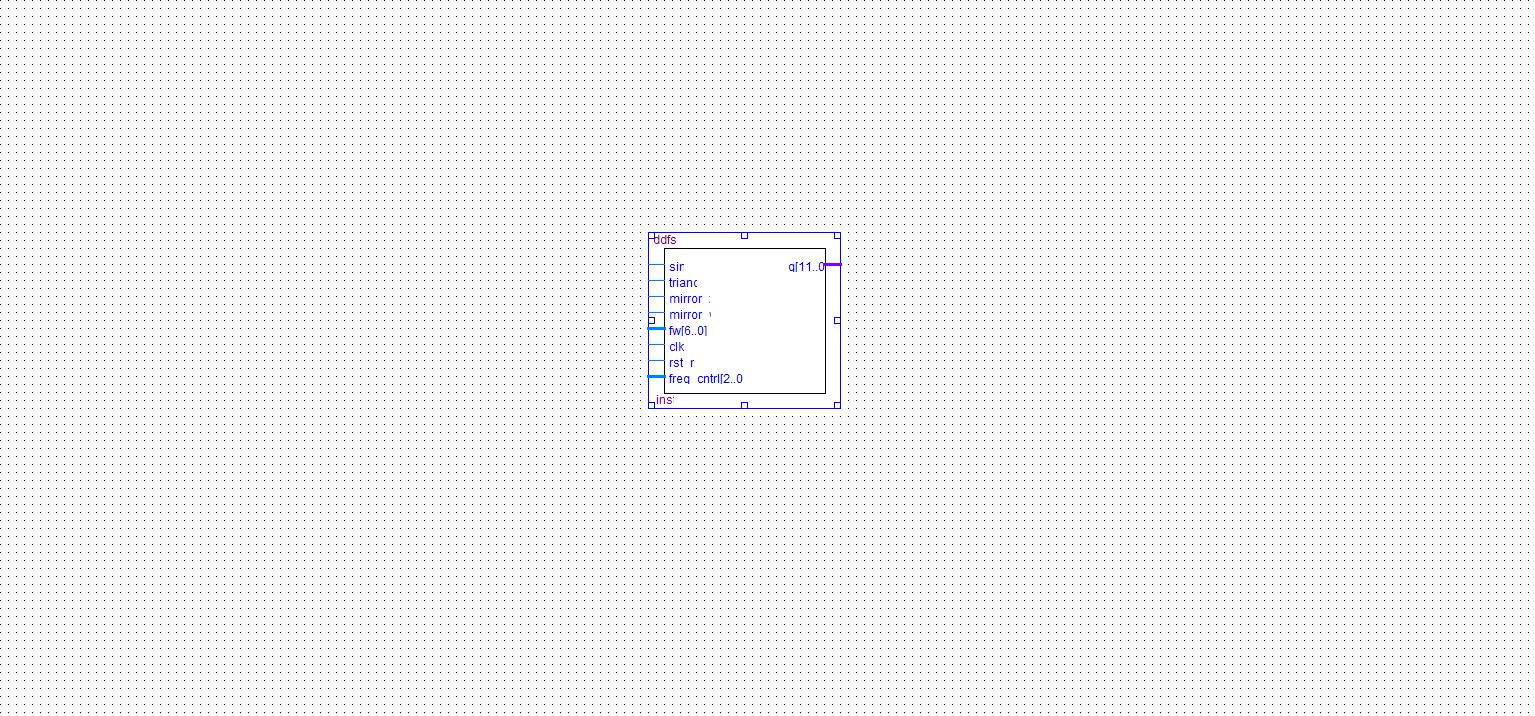
\includegraphics[width=\textwidth, trim={12cm 5.5cm 13cm 4cm}, clip]{img/DDFS_12bit.jpg}
    \end{minipage}
    \hfill
    % Immagine a destra (uguale)
    \begin{minipage}{0.45\textwidth}
        \centering
        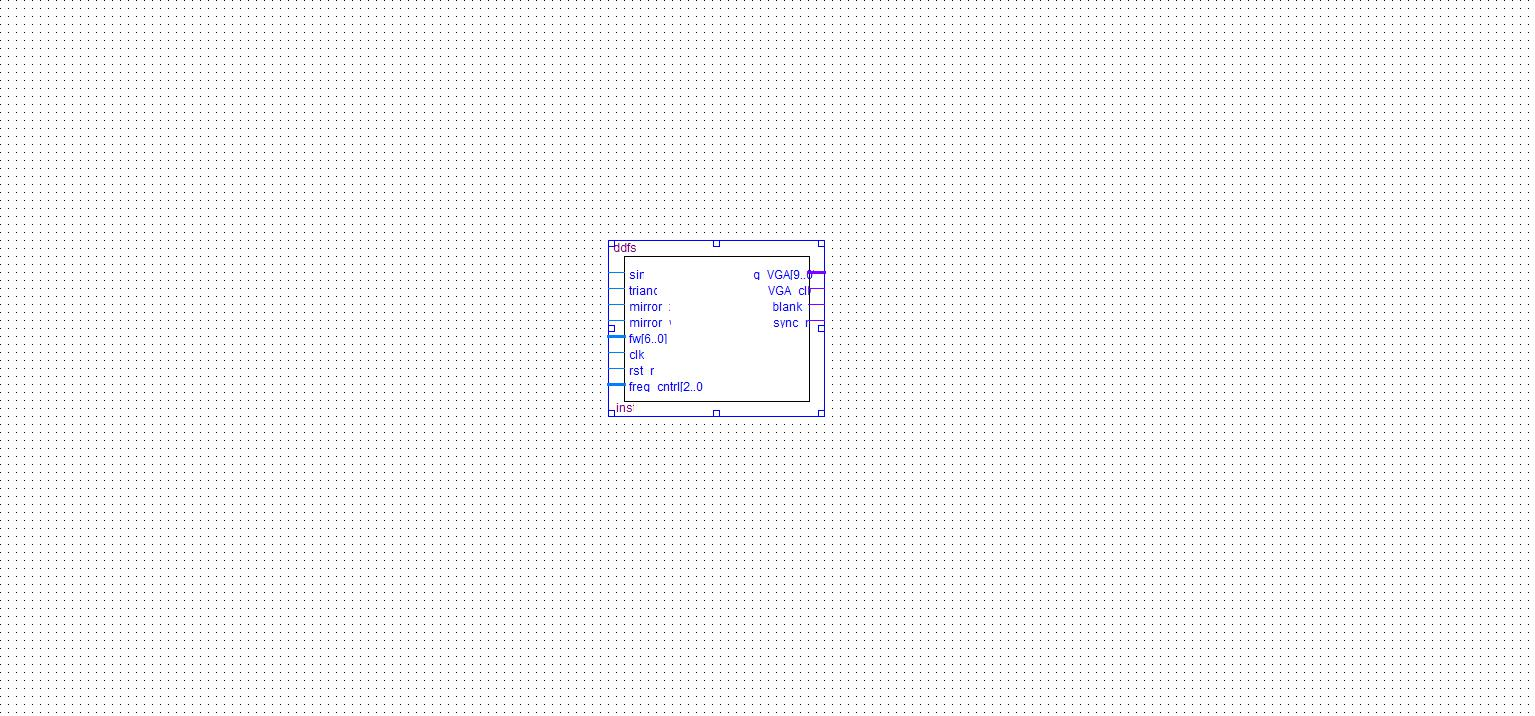
\includegraphics[width=\textwidth, trim={11.5cm 5cm 13cm 4cm}, clip]{img/DDFS_VGA.jpg}
    \end{minipage}

    \caption{DDFS module}
    \label{fig:DDFS_module}
\end{figure}
\vspace*{0.5cm}

\paragraph{I/O interface} \quad \\
The ports used to connect this module to other modules or to the external pins of the FPGA are the following:

\begin{itemize}

    \item \texttt{sin, tri} \\
    used to select the output waveform. If \texttt{sin} and \texttt{tri} are both zero, the output signal is a square wave. The sinusoidal output has priority.
    
    \item \texttt{mirror\_x, mirror\_y} \\
    used to manually select the symmetry of the output wave. \texttt{mirror\_x} is used to enable the horizontal symmetry of the wave, and \texttt{mirror\_y} to enable the vertical symmetry. For every symmetry pin enabled, the period of the output wave doubles because the wave needs to be repeated mirrored.
    
    \item \texttt{f\_w} \\
    is the value of the frequency word. It is composed of \(7bits\) and is 
    \texttt{unsigned}, so the maximum value is \(2^7 - 1 = 127\). The instantiated LUT is a \((12 \ \text{x} \ 1024)bit\) memory where the address value goes from \(0\) to \(1023\), and the stored samples are \(12bit\) values. The number of samples sent to the DAC after a complete scan cycle are \( 8 < \frac{1024}{\texttt{f\_w} + 1} < 1024 \).
    
    \item \texttt{clk, rst\_n} \\
    are the clock and the synchronous reset pins.
    
    \item \texttt{freq\_cntrl} \\
    is a select input used to scale the clock frequency by a fixed value.
    It is a \(3bit\) input pin, and the scalable frequency values are \(\frac{f_{clk}}{1^. 000^. 000}\), \(\frac{f_{clk}}{100^. 000}\), \(\frac{f_{clk}}{10^. 000}\), ... \(\frac{f_{clk}}{100}\), \(\frac{f_{clk}}{10}\), \(\frac{f_{clk}}{2}\).
    The total scalable frequencies are \(7\), and they are associated with the values of \texttt{freq\_cntrl} from \(0\) to \(6\).

    \item \texttt{q} or \texttt{q\_VGA, blank, sync\_n, VGA\_clk} \\
    are the digital output values. For the first version, \texttt{q} is a \(12bit\) value synchronized with the divided value of the clock. \\
    For the VGA\_DAC, the \texttt{q\_VGA} output is a \(10bit\) bus, so the 2 least significant bits are truncated.
    The VGA\_DAC also needs to be synchronized with a clock to sample the values, so the output of the frequency divider has been connected to the \textbf{phase accumulator} and \texttt{VGA\_clk}. The \texttt{blank} and \texttt{sync\_n} signals are connected to 1 because they are not used.
    
\end{itemize}

\paragraph{Verilog code} \quad \\
In the first part of the module is declared a \(12 bits\) register where is stored a quarter of the wave to show. \\
The content of the register depend on the output waveform selected.

\vspace{1cm}
\begin{lstlisting}[language=Verilog, caption=Selection of the output waveform, 
label=lst:DDFS_q_tmp ]
    reg [11:0] q_tmp;
    localparam HALF_ADDRESS = 2**(ADDR_WIDTH-1);
    always @(*) begin
        
        if(sin)
            q_tmp = lut_out;     //sinusoidal output
        else if(triang)
            q_tmp = addr*(12'hfff/(MAX_LUT-1));      //triangular output	
        else
            q_tmp = 12'hfff;     //square output
    
    end
\end{lstlisting}
\vspace{1cm}

\noindent
if the sinusoidal wave is selected, the register is loaded with the output of the LUT.
The triangular wave is calculated multiplying the address value of the LUT with a coefficient that allow it to go from \texttt{0x000} to \texttt{0xFFF} that is the full range of the digital value. \\
The quarter triangular-wave is calculated as follow 

\vspace{0.5cm}
\[
    \texttt{out} = \texttt{address} \cdot \frac{\texttt{0xFFF}}{max(\texttt{address})} = \texttt{address} \cdot \frac{\texttt{0xFFF}}{\texttt{MAX\_LUT} - 1}
\] 
\vspace{0.5cm}

\noindent
A quarter of a square-wave is a constant value, so in this case the output is \texttt{0xFFF}.

\newpage
\noindent
In the second part is defined the \textbf{phase accumulator}, the counter need to be four times larger than the maximum address of the LUT, because in the worst case where are enabled both of the symmetry the period of the wave is \(4 \cdot T\) where \(T\) is the period of the quarter wave stored in the LUT. \\
The LUT have a 1 clock cycle latency after the read request, for this reason has been defined a counter re-timed with a clock cycle synchronized with the LUT output.

\vspace{1cm}
\begin{lstlisting}[language=Verilog, caption=Address calculation with vertical mirroring, 
label=lst:DDFS_address ]
    //retiming register for address counter
    reg [ADDR_WIDTH+1:0] cont_rt;
    always @(posedge clk_div)
        cont_rt <= cont;
    
    //calculate address
    always @(*) begin
        
        //not mirrored case
        addr = cont%(MAX_LUT);
        
        //y mirrored output
        if(mirror_y)
            //second quarter or fouth quarter
            if(
            (cont > (MAX_LUT-1)) && (cont <= (2*MAX_LUT-1)) ||
            (cont > (3*MAX_LUT-1)) && (cont <= (4*MAX_LUT-1))
            )
                addr = (MAX_LUT-1) - cont%(MAX_LUT);
                
    end
\end{lstlisting}
\vspace{1cm}

\noindent
When mirroring is disabled, the address is equal to \(|\texttt{counter}|_{\texttt{MAX\_LUT}}\). \\
To simplify hardware synthesis, \texttt{MAX\_LUT} is better chosen as a power of two; in this case, the modulo operation becomes simply a truncation of the most significant bits. \\
When vertical mirroring is enabled, the circuit checks the address counter to determine the quarter of the wave to display, and when the signal is in the third or fourth quarter, the address sweeps from the last entry of the LUT to the first one.

\vspace{\baselineskip}

\noindent
In the last part of the module, the output with horizontal symmetry is calculated. \\
To allow the output to be represented with \(12 bits\) under horizontal symmetry, starting from a \(12 bit\) sample, the output is divided by two and summed with an offset constant equal to half of the total output swing.

\begin{center}

    \vspace*{0.5cm}
    \scalebox{0.9}{
        \begin{minipage}{0.49\textwidth}
            \begin{tikzpicture}[scale=0.7]
                \begin{axis}[
                    axis lines = middle,
                    xlabel = {$t$},
                    ylabel = {},
                    xmin = 0, xmax = 2*pi+0.5,
                    ymin = -0.1, ymax = 1.1,
                    samples = 200,
                    title = {Waveform without Horizontal Symmetry},
                    xtick = {pi/2, pi, 3*pi/2, 2*pi},
                    xticklabels = {$\frac{1}{4f_o}$, $\frac{1}{2f_o}$, $\frac{3}{4f_o}$, $\frac{1}{f_o}$},
                    ytick = {0, 1},
                    yticklabels = {0, $f_{max}$}
                ]
                
                \addplot [red, thick, domain=0:2*pi] {abs(sin(deg(x)))};
                
                \end{axis}
                
            \end{tikzpicture}
        \end{minipage}
        \hfill
        \begin{minipage}{0.49\textwidth}
            \begin{tikzpicture}[scale=0.7]
                \begin{axis}[
                    axis lines = middle,
                    xlabel = {$t$},
                    ylabel = {},
                    xmin = 0, xmax = 2*pi+0.5,
                    ymin = -0.1, ymax = 1.1,
                    samples = 200,
                    title = {Waveform with Horizontal Symmetry},
                    xtick = {pi/2, pi, 3*pi/2, 2*pi},
                    xticklabels = {$\frac{1}{4f_o}$, $\frac{1}{2f_o}$, $\frac{3}{4f_o}$, $\frac{1}{f_o}$},
                    ytick = {0, 0.5, 1},
                    yticklabels = {0, $\frac{f_{max}}{2}$, $f_{max}$}
                ]
                
                \addplot [blue, thick, domain=0:2*pi] {(sin(deg(x)) + 1)/2};
                \addplot [cyan, thick, domain=0:2*pi] {0.5};
                
                \end{axis}
                
            \end{tikzpicture}
        \end{minipage}
    }
    \vspace*{0.5cm} 

\end{center}

\noindent
The operation performed to the output is \(\texttt{out} = \frac{q}{2} + \frac{f_{max}}{2} = \frac{\texttt{q}}{2} + \texttt{HALF\_DATA} \).
When the horizontal symmetry is enabled the output must be inverted, so the output is \(\texttt{out} = -\frac{q}{2} + \frac{f_{max}}{2} = -\frac{\texttt{q}}{2} + \texttt{HALF\_DATA} \).

\vspace{1cm}
\begin{lstlisting}[language=Verilog, caption=Output calculation with horizontal mirroring, 
label=lst:DDFS_output_calculation ]
    //calculate the output
    reg [ADDR_WIDTH+1:0] act_cont;
    localparam HALF_DATA = 2**(DATA_WIDTH-1);
    always @(*) begin
    
        //not mirrored case
        q = HALF_DATA + (q_tmp >> 1) - 1;
        
        //select the correct counter for the wave we are using
        if(sin)
            act_cont = cont_rt;
        else 
            act_cont = cont;
        
        if(mirror_x && mirror_y) begin
            //third quarter or fourth quarter
            if( 
            ((act_cont > (2*MAX_LUT-1)) && (act_cont <= (3*MAX_LUT-1))) || 
            ((act_cont > (3*MAX_LUT-1)) && (act_cont <= (4*MAX_LUT-1))) 
            )
                q = HALF_DATA - (q_tmp >> 1) - 1;
                
        end else if(mirror_x) begin
            //second quarter or fourth quarter
            if(
            ((act_cont > (MAX_LUT-1)) && (act_cont <= (2*MAX_LUT-1))) || 
            ((act_cont > (3*MAX_LUT-1)) && (act_cont <= (4*MAX_LUT-1))) 
            )
                q = HALF_DATA - (q_tmp >> 1) - 1;
        
        end
            
    end
\end{lstlisting}
\vspace{1cm}

\noindent
The horizontal symmetry needs to be applied during the second and fourth quarters when vertical symmetry is not enabled. \\
When vertical symmetry is enabled, the period of the wave is \(2 \cdot T\), and horizontal symmetry must be applied in the third and fourth quarters. \\
To calculate the address, a global counter is used, and is performed the modulo operation with base \texttt{MAX\_LUT}.

\newpage
\noindent
The problem with this technique is that when the address moves from one quarter to another, if \texttt{f\_w} is greater than one, the address can start from a value bigger than zero. \\
For example, if \texttt{MAX\_LUT} is \(1024\) and \texttt{cont} is \(1000\), with \texttt{f\_w} equal to \(600\), the next value of \texttt{cont} is \(1000 + 600 = 1600\).\\
This means that \texttt{address} is equal to \texttt{cont} when it is \(1000\), but at the next clock cycle it becomes \(|1600|_{1024} = 576\).\\
Therefore, the \texttt{address} starts counting from \(0\), and in the next quarter of the wave it starts from \(576\).\\
This behavior causes the output waveform to be slightly different from period to period.\\
To avoid this, when the \texttt{address} is about to overflow, the \texttt{counter} is set to a multiple of \texttt{MAX\_LUT}, so that at the next cycle the \texttt{address} starts from \(|N \cdot 1024|_{1024} = 0\).

\vspace{1cm}
\begin{lstlisting}[language=Verilog, caption=Calculation of counter for DDFS address, 
label=lst:DDFS_cont_calculation ]
    if(cont < MAX_LUT-1) begin
        if(cont + (fw+1) >= MAX_LUT-1)
            cont <= MAX_LUT;
        else
            cont <= cont + (fw+1);
    end
    else if(cont < 2*MAX_LUT-1) begin
        if(cont + (fw+1) >= 2*MAX_LUT-1)
            cont <= 2*MAX_LUT;
        else
            cont <= cont + (fw+1);
    end
    else if(cont < 3*MAX_LUT-1) begin
        if(cont + (fw+1) >= 3*MAX_LUT-1)
            cont <= 3*MAX_LUT;
        else
            cont <= cont + (fw+1);
    end
    else if(cont < 4*MAX_LUT-1) begin
        if(cont + (fw+1) >= 4*MAX_LUT-1)
            cont <= 0;
        else
            cont <= cont + (fw+1);
    end
    else
        cont <= 0;
\end{lstlisting}
\vspace{1cm}

\paragraph{Sub-modules} \quad \\
Inside this module are instantiated two other modules

\begin{itemize}
    \item \textbf{Programmable frequency divider} to scale the clock frequency to lower values
    \item \textbf{Look Up Table} to store the digital samples for sinusoidal output
\end{itemize}

\newpage

\paragraph{Programmable frequency divider} \quad \\
We implemented a scalable frequency divider controlled by the \texttt{freq\_ctrl} \(3 bit\) signal to divide the output frequency with a coefficient ranging from \(2\) to \(1000000\).\\
This is useful to maintain a decent quality of the output wave, even with higher values of the frequency word.\\
With this method, using an input frequency of \(50MHz\), we can select the output frequencies of \(25MHz\), \(5MHz\), \(500kHz\), \(50kHz\), \(5kHz\), \(500Hz\), and \(50Hz\).\\
A \(20 bit\) counter is used, and the output is connected to the MSB of the counter.\\
The output clock is then generated with a \(0.5\) duty cycle by starting the counter when the MSB is 0 and, after half of the counter period, the MSB becomes 1; then the counter resets to the start.\\
When \texttt{freq\_ctrl} changes, the \texttt{start\_cnt} and \texttt{end\_cnt} registers are updated, and thus the counter restart condition also changes, avoiding conflicts.


\vspace{1cm}
\begin{lstlisting}[language=Verilog, caption=Programmable frequency divider,
    label=lst:Prog_freq_div ] 
    always @(posedge clk_in) begin
        if(rst_n == 1'b0) begin
            count <= start_cnt;
        end else if(count >= (end_cnt-1'b1))begin
            count <= start_cnt;
        end else begin
            count <= count + 1'b1; 	
        end
        
    end

    always @(*) begin
    
        case (freq_cntrl)
            
            0:begin 
                start_cnt = 20'h80000-1;
                end_cnt = start_cnt+2; 
            end
            1:begin
                start_cnt = 20'h80000-10/2;
                end_cnt = start_cnt + 10;
            end
            .
            .
            .
            
            6:begin
                start_cnt = 20'h80000-1000000/2;
                end_cnt = start_cnt + 1000000;
            end
            default:begin
                start_cnt = 20'h80000-1000000/2;
                end_cnt = start_cnt + 1000000;
            end
            
        endcase 
    
        clk_out = count[19];
        
    end
    
\end{lstlisting}
\vspace{1cm}

\newpage

\paragraph{Look Up Table} \quad \\
The LUT is a pre-initialized ROM instantiated inside the FPGA with the samples of a quarter of a sinusoidal wave. \\
The samples stored in the ROM are \(12 bit\) samples calculated as follows 

\vspace{0.5cm}
\[
    \texttt{sample}[n]_{12 bit} = sin\left(\frac{n}{\texttt{LUT\_DIM} - 1} \cdot \frac{\pi}{2}\right)_{12 bit}
\]
\vspace{0.5cm}

\noindent
The \texttt{LUT\_DIM} is choose to be \(2^{10}\), so the LUT is a \((12 \text{x} 1024) bit\) ROM inside the FPGA.

\newpage
\subsubsection{Keypad frequency select module}

This module reads the button pressed on the keypad every \(N\) clock cycles. \\
The keypad is used to enter the frequency of the wave, and the output of this module is the frequency in BCD or \textbf{binary-coded decimal} representation. \\
Inside the module, there is a converter network that converts the frequency value into a combination of \texttt{f\_w} and \texttt{freq\_cntrl}, which are the inputs of the DDFS module used to control the output wave frequency.

\vspace{0.5cm}
\begin{figure}[h!]
    \centering
    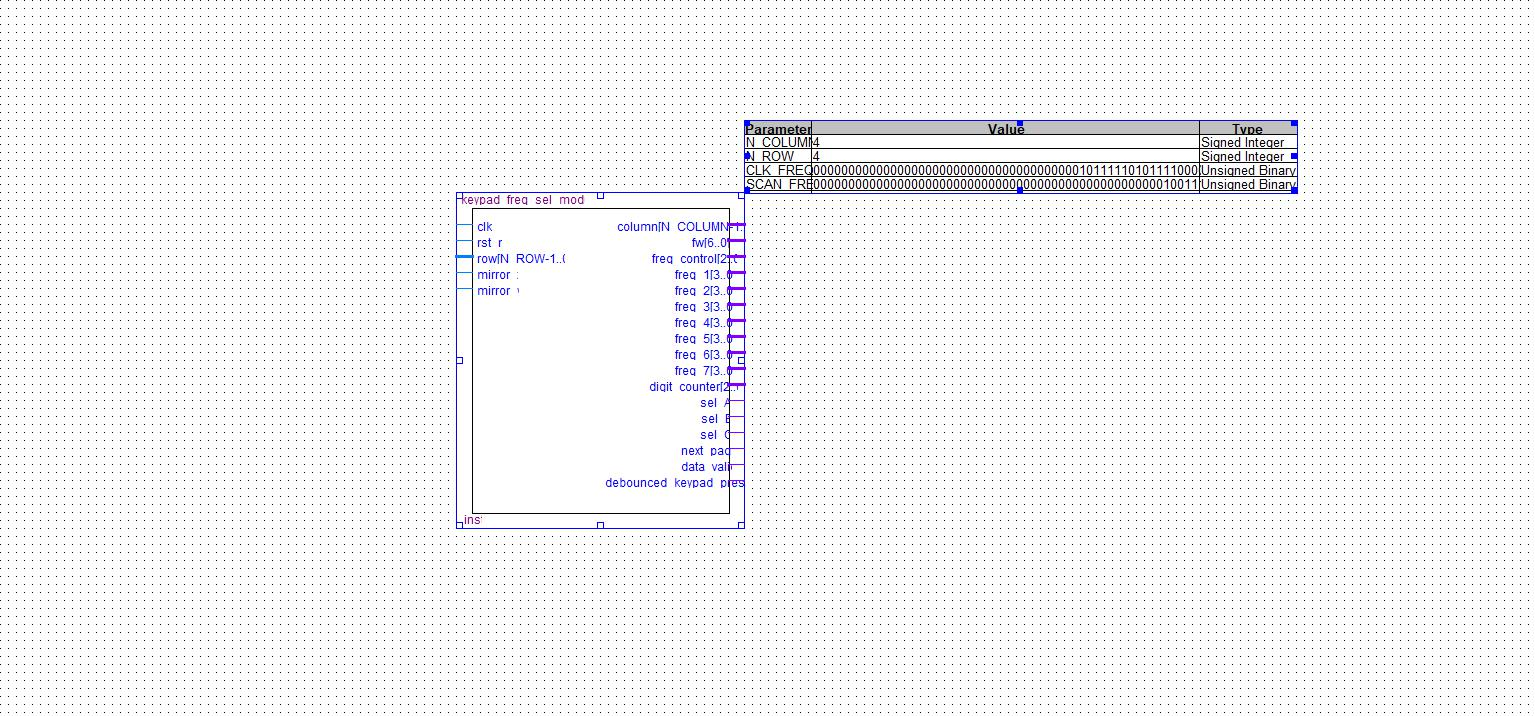
\includegraphics[width=0.8\textwidth, trim={8cm 3cm 3cm 1.5cm}, clip]{img/keypad_freq_sel.jpg}
    \caption{Keypad frequency select module}
    \label{fig:keypad_module}
\end{figure}
\vspace{0.5cm}

\paragraph{I/O interface} \quad \\
The ports used to connect this module to other modules or to the external pins of the FPGA are the following:

\begin{itemize}

    \item \texttt{clk, rst\_n} \\
    are the clock and the synchronous reset pins.

    \item \texttt{row} \\
    this is the input pin from the keyboard. \\
    This pins need to be connected to the internal pullup of the FPGA, because the keypad matrix, when a button is not pressed, leave the line floating. \\
    Every bit of this word is connected to a row line of the keypad.

    \item \texttt{mirror\_x, mirror\_y} \\
    these are the mirroring pins of the output wave; if the output wave is mirrored, the LUT must be read two or four times (depending on how many mirroring effects are applied to the wave) every period. \\
    This means that the \texttt{f\_w} and \texttt{freq\_control} values depend on the value of \texttt{mirror\_x} and \texttt{mirror\_y}.
    

    \item \texttt{column} \\
    this output pin is connected to the keypad, and is used to enable the column before reading a row. \\
    By enabling a column and reading the row values is possible to determine which button is pressed.

    \item \texttt{f\_w, freq\_control} \\
    this outputs goes to the DDFS module to set the frequency of the output wave.

    \item \texttt{freq\_1, freq\_2, ... ,freq\_7} \\
    this is the 7 digits of the output frequency expressed in BCD representation.

    \item \texttt{digit\_counter} \\
    this output represent the number of the frequency digits.

    \item \texttt{sel\_A, sel\_B} \\
    these outputs are toggled every time the A and B buttons of the keypad are pressed. \\
    This can be useful because the VGA DAC has three \(10 bit\) inputs, so it is possible to instantiate two DDFS modules connected to each DAC input, and these pins can individually enable each DDFS module.

    \item \texttt{next\_page, prev\_page} \\
    this output is connected to LCD module to change the wave to be visualized.

    \item \texttt{data\_valid, debounced\_keypad\_pressed} \\
    are test outputs used for debugging.
    
\end{itemize}

\paragraph{Parameters} \quad \\
The parameters of this module are:

\begin{itemize}

    \item \texttt{N\_COLUMN, N\_ROW} \\
    are the number of rows and column of the keypad module used

    \item \texttt{SCAN\_FREQ} \\
    this is the frequency used to perform the keypad scanning. \\
    If the scan operation is performed too rapidly, the parasitic capacitance of the buttons, in series with the pull-up resistors, can create reading problems. \\
    The scan frequency value used is \(10kHz\).

    \item \texttt{CLK\_FREQ} \\
    is the clock frequency of the clock connected to this module. \\
    Is used to synchronize the timers for the debounce circuit and the scanning frequency of the keypad.
    
\end{itemize}

\paragraph{Verilog code} \quad \\
The module is made of a single sequential network that checks every clock cycle whether the \texttt{data\_valid} signal (from the sub-module that reads the keypad buttons) is high, and reads which button is pressed in that case. \\
The first problem is that the button bounces significantly before stabilizing in one position. \\
For this reason, a debounce circuit has been implemented, with a timer that waits for approximately \(100ms\) after the button is pressed before considering the button as pressed.

\vspace{0.5cm}
\begin{lstlisting}[language=Verilog, caption=Debounce circuit, 
label=lst:debounce_circuit ]
    always @(posedge clk) begin
        if(rst_n == 0) begin
            //reset condition
            debounce_cont <= 0;
            debounced_keypad_pressed <= 1'b0;
        end else if(clk_ena == 1) begin
            if(out_keys == 16'd0) begin
                debounce_cont <= 0;
                debounced_keypad_pressed <= 1'b0;
                out_keys_sync <= out_keys_sync;
            end else begin
                debounce_cont <= debounce_cont + 1;
                if(debounce_cont >= DEBOUNCE_CYCLE) begin
                    debounce_cont <= DEBOUNCE_CYCLE;
                    debounced_keypad_pressed <= 1'b1;
                    out_keys_sync <= out_keys;
                end
            end
        end else begin
            debounce_cont <= debounce_cont;
            debounced_keypad_pressed <= debounced_keypad_pressed;
            out_keys_sync <= out_keys_sync;
        end
    end
\end{lstlisting}
\vspace{0.5cm}

\newpage
\noindent
The second problem is that a button is usually pressed for too long; for this reason, a flag has been instantiated to check if the button has been released. \\
This flag makes it possible to perform an action only once, even if the button remains pressed for many clock cycles.

\vspace{0.5cm}
\begin{lstlisting}[language=Verilog, caption=Flag to avoid multiple operation with a single press, 
label=lst:pressed_button_flag ]
    if(data_valid == 1) begin   
        if(debounced_keypad_pressed == 0) begin
            //flag reset
            button_pressed <= 1'b0;
        end
        if(debounced_keypad_pressed == 1 && button_pressed == 0) begin
    
            .
            .
            .
            
            //flag set
            button_pressed <= 1'b1;
        end
    end
\end{lstlisting}
\vspace{1cm}

\noindent
Now we have to define the behavior of the machine upon the press of each button. \\
When multiple buttons are pressed simultaneously, the machine does nothing by default. \\
When a number is pressed, the machine shifts the digits of the frequency number to the left and writes the pressed number in the place of the least significant digit. \\
If a new number have to be selected, the flag \texttt{number\_not\_sel} is high and the number become the digit pressed.

\vspace{0.5cm}
\begin{lstlisting}[language=Verilog, caption=Number digit pressed on the keypad, 
label=lst:number_key_pressed ]
    // ---- NUMBER KEY PRESSED ---- //
    
    (16'd1 << 0): begin
        if(number_not_sel == 1) begin
            {freq_7, freq_6, freq_5, freq_4, freq_3, freq_2, freq_1} <= 1;
            digit_counter <= 3'd1;
            number_not_sel <= 1'b0;
        end else if(digit_counter < 7) begin
            //shift right and write the first digit
            {freq_7, freq_6, freq_5, freq_4, freq_3, freq_2, freq_1} <=
            {freq_6, freq_5, freq_4, freq_3, freq_2, freq_1, 4'd1};
            //increase the number of digit
            digit_counter <= digit_counter + 1;
        end
    end
    
    .
    .
    .
    
    // ---- DEFAULT CONDITION ---- //
                
    default: begin
        {freq_7, freq_6, freq_5, freq_4, freq_3, freq_2, freq_1} <=
        {freq_7, freq_6, freq_5, freq_4, freq_3, freq_2, freq_1};
        digit_counter <= digit_counter;
    end 
\end{lstlisting}
\vspace{0.5cm}

\newpage
\noindent
The letter buttons toggle the \texttt{sel\_A} and \texttt{sel\_B} outputs, the C and D buttons of the keypad are used to send the next page or previous page signals to the LCD module. \\
The last two buttons of the keypad are used to confirm the frequency value written
or to erase the digits.

\vspace{0.5cm}
\begin{lstlisting}[language=Verilog, caption=Confirm or erase button pressed on the keypad, 
label=lst:confirm_erase_key_pressed ]
    // ---- CONFIRM OR ERASE KEY PRESSED ---- //
                    
    (16'd1 << 14): begin
        if(digit_counter > 0) begin
            //digit erased, shift left the digit
            {freq_7, freq_6, freq_5, freq_4, freq_3, freq_2, freq_1} <=
            {4'd0, freq_7, freq_6, freq_5, freq_4, freq_3, freq_2};							
            //decrease the number of digit
            digit_counter <= digit_counter - 1;
        end
        else begin
            {freq_7, freq_6, freq_5, freq_4, freq_3, freq_2, freq_1} <=
            {BCD_7, BCD_6, BCD_5, BCD_4, BCD_3, BCD_2, BCD_1};
            //store the previous number of digit
            digit_counter <= digit_counter_BCD;
            number_not_sel <= 1'b1;
        end
    end 
    
    (16'd1 << 12): begin
        //frequency confirmed, save the frequency value
        {BCD_7, BCD_6, BCD_5, BCD_4, BCD_3, BCD_2, BCD_1} <= 
        {freq_7, freq_6, freq_5, freq_4, freq_3, freq_2, freq_1};
        //load the actual number of digit
        digit_counter_BCD <= digit_counter;
        number_not_sel <= 1'b1;
    end 
\end{lstlisting}
\vspace{0.5cm}

\noindent
When a value is confirmed, the flag \texttt{number\_not\_sel} is set to one, so when a digit is pressed, the new number starts to be written from the least significant digit. \\
When a digit is erased, the number is shifted to the right and the most significant digit become a zero.

\newpage

\paragraph{Sub-modules} \quad \\
Inside this module are instantiated three other modules

\begin{itemize}
    \item \textbf{Keypad reader module} to read the button values of the keypad.
    \item \textbf{BCD to C1 converter} to convert the frequency value from BCD to C1 representation.
    \item \textbf{DDFS frequency converter} to convert the C1 frequency value into a combination of \texttt{f\_w} and \\
    \texttt{freq\_control} used to control the DDFS module.
\end{itemize}

\paragraph{Keypad reader module} \quad \\
This module uses a shift register connected to the column lines to enable a different column every clock cycle. \\
The logic is reversed: a column is considered enabled when it is pulled low, and a row is considered active when the line value is low. \\
This choice was made because the FPGA GPIOs can be defined with internal \(25 k\Omega\) pull-up resistors but no internal pull-downs. \\
After \(N_{col}\) clock cycles, where \(N_{col}\) is the number of columns of the keypad, the controller pulls up the \texttt{data\_valid} pin to indicate that the output of the module contains the pressed button. \\
Every clock cycle, a counter called \texttt{i\_column} increases, and when the value of the counter reaches \(N_{col}\), it activates \texttt{data\_valid}. \\
At each clock cycle, a different column is enabled, and the value of the pressed row is stored in an output vector called \texttt{out\_keys}. \\
The structure of the output value is a \texttt{bidimensional-vector}, that has been implemented using a technique called \textbf{array flattening}. \\
The array flattening technique consists of dividing the array into consecutive sub-arrays representing the rows of the matrix, where the columns correspond to the values inside the sub-arrays. \\
The flattened array contains \(N_{col} \cdot N_{row}\) elements, and the index of each element is calculated from the \(i_{col}\) and \(i_{row}\) indices using the following formula \( i = N_{row} \cdot i_{col} + i_{row}\).

\vspace{0.5cm}
\begin{figure}[h!]
    \centering
    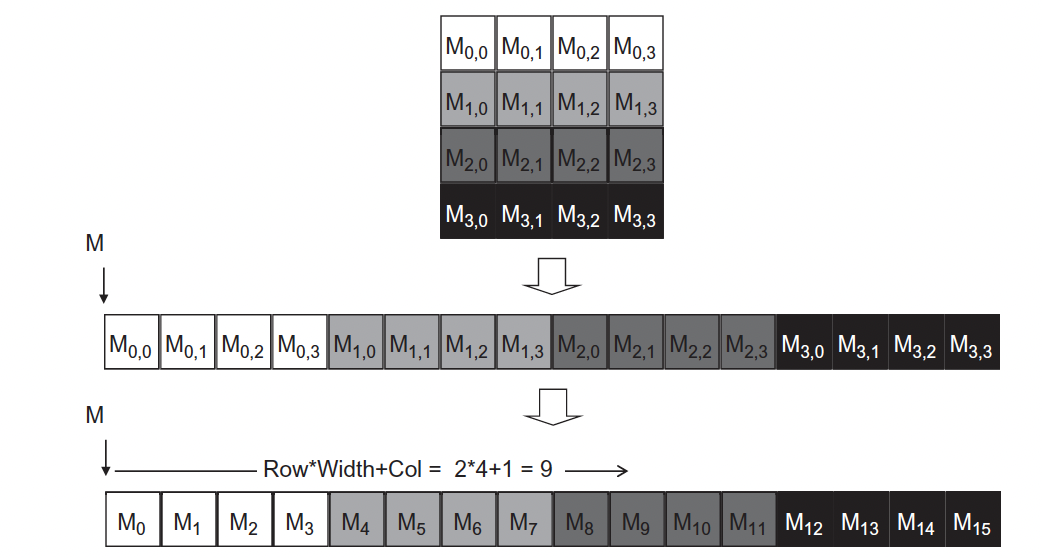
\includegraphics[width=0.8\textwidth, clip]{img/array flattening.png}
    \caption{Array flattening technique}
    \label{fig:arr_flat}
\end{figure}
\vspace{0.5cm}

\newpage
\noindent
The shift register connected to the columns is implemented with a combinatorial network that reads the value of \texttt{i\_column} and pulls down the corresponding line. \\
To prevent the module from sampling the row values too close to the change of column enable, the \texttt{i\_column} values range from \(0\) to \(2 \cdot \texttt{N\_COLUMN}\). \\
When \texttt{i\_column} is odd, the column is enabled; when it is even, the row is read. \\
By doing this, the reading operation occurs one clock cycle after the column enabling operation.


\vspace{0.5cm}
\begin{lstlisting}[language=Verilog, caption=Shift register implementation ]
    //assign the output values at the column of the keypad
    integer i;
    always @(*) begin
        //default values
        i = 0;
        column = ~0;
        
        //check if i_column is in range
        if(i_column <= 2*N_COLUMN) begin
            for(i=0; i<N_COLUMN; i=i+1) begin
                if(i == (i_column >> 1)) begin
                    column[i] = 0;
                end else begin
                    column[i] = 1;
                end
            end
        end
        
    end
\end{lstlisting}
\vspace{0.5cm}

\noindent
Another combinatorial network updates a flattened vector that contains the button pressed for the currently enabled column.

\vspace{0.5cm}
\begin{lstlisting}[language=Verilog, caption=Button reading implementation]
    //read the button values from the keypad
    integer i_col, i_row;
    always @(*) begin
        //default values
        i_col = 0;
        i_row = 0;
        
        //read button cycles
        for(i_col=0; i_col<N_COLUMN; i_col=i_col+1) begin
            for(i_row=0; i_row<N_ROW; i_row=i_row+1) begin
                if(row[i_row] == 0 && i_col == (i_column >> 1)) begin
                    key_pressed[i_col*N_ROW + i_row] = 1; 
                end else begin
                    key_pressed[i_col*N_ROW + i_row] = 0; 
                end
            end
        end
        
    end
\end{lstlisting}
\vspace{0.5cm}

\noindent
Every two clock cycle, the output vector is updated with the button pressed for each column and after \(2 \cdot N_{col}\) cycles the reading cycle is done and data output is valid.

\newpage
\noindent
The two main issues encountered when reading the keypad are:
\begin{itemize}
    \item The button press event is asynchronous.
    \item The scan frequency cannot be too high due to the parasitic capacitance of the buttons and the pull-up resistors.
\end{itemize}

\noindent
For the first issue, the module provides a flip-flop chain directly connected to the keypad inputs, reducing the probability of metastability problems.

\vspace{0.5cm}
\begin{lstlisting}[language=Verilog, caption=flip-flop chain to reduce metastability problem occur]
    //latch chain to reduce metastability problems
    reg [N_ROW-1:0] row_1, row_2, row_sync;
    always @(posedge clk) begin
        if(rst_n == 0) begin
            //reset condition
            row_1 <= 0;
            row_2 <= 0;
            row_sync <= 0;
        end
        else begin
            row_sync <= row_2;
            row_2 <= row_1;
            row_1 <= row;
        end
    end
\end{lstlisting}
\begin{center}
    \vspace{0.5cm}
    \scalebox{0.7}{
        \begin{tikzpicture}
        	% Paths, nodes and wires:
        	\node[flipflop D, fill=cyan!30!white] at (3.12, 5.16){};
        	\node[flipflop D, fill=cyan!30!white] at (7.13, 5.16){};
        	\node[flipflop D, fill=cyan!30!white] at (11.13, 5.16){};
        	\draw (4.25, 6) -- (6, 6);
        	\draw (8.25, 6) -- (10, 6);
        	\draw (2, 6) |- (1, 6);
        	\draw (6.01, 4.32) -| (5.25, 3);
        	\draw (10.01, 4.32) -| (9.25, 3);
        	\draw (9.25, 3) -- (1, 3);
        	\draw (2, 4.32) -| (1.25, 3);
        	\draw (1, 3) -- (0.25, 3);
        	\draw (1, 6) -- (0.25, 6);
        	\node[circ] at (5.25, 3){};
        	\node[circ] at (1.25, 3){};
        	\node[shape=rectangle, minimum width=0.715cm, minimum height=0.465cm] at (0.625, 6.25){} node[anchor=north west, align=left, text width=0.327cm, inner sep=6pt] at (0.25, 6.5){in};
        	\node[shape=rectangle, minimum width=0.84cm, minimum height=0.465cm] at (0.563, 3.25){} node[anchor=north west, align=left, text width=0.452cm, inner sep=6pt] at (0.125, 3.5){clk};
        	\draw (13.25, 6) |- (12.25, 6);
        	\node[shape=rectangle, minimum width=0.965cm, minimum height=0.465cm] at (13, 6.25){} node[anchor=north west, align=left, text width=0.577cm, inner sep=6pt] at (12.5, 6.5){out};
        \end{tikzpicture}
    }
    \vspace{0.5cm}
\end{center}

\noindent
To solve the second issue, the module includes a clock enable signal generated by an internal counter. Each time the clock enable signal is asserted, the synchronized operations are performed. \\
The clock enable signal is also forwarded to the keypad frequency selection module.

\vspace{0.5cm}
\begin{lstlisting}[language=Verilog, caption=Clock enable signal generation]
    //clock enable generator
    localparam FREQ_DIV = (CLK_FREQ/SCAN_FREQ>3) ? CLK_FREQ/SCAN_FREQ : 3;
    integer clock_div_cont;
    always @(posedge clk) begin
        if(rst_n == 0) begin
            //reset condition
            clock_div_cont <= 0;
            clk_ena <= 1'b0;
        end
        else begin
            clock_div_cont <= clock_div_cont + 1;
            clk_ena <= 1'b0;
            if (clock_div_cont >= FREQ_DIV) begin
                clock_div_cont <= 0;
                clk_ena <= 1'b1;
            end
        end
    end
\end{lstlisting}
\vspace{0.5cm}

\noindent
The flip-flop chain introduces a delay, as the output data is delayed with respect to the input data by three clock cycles.\\
For this reason, the \texttt{FREQ\_DIV} parameter is defined to be greater than three, ensuring that the output delay introduced by the chain is absorbed before the next reading operation.

\paragraph{BCD to C1 converter} \quad \\
This module takes as input the value to be converted from BCD representation and converts it into a C1 representation value. \\
To perform this operation, the value must be calculated as follows

\[
    n_{C1} = \sum_{i=0}^{\texttt{n\_digit}} a_i \cdot 10^i
\]

\noindent
This operation instantiates many multipliers, which are hardware-expensive; for this reason, every power of \(10\) is decomposed into a sum of powers of two

\[
    n_{C1} = \sum_{i=0}^{\texttt{n\_digit}} a_i \cdot 10^i
           = \sum_{i=0}^{\texttt{n\_digit}}
             \left[ a_i \cdot \left( \sum_{j} b_j \cdot 2^j \right) \right] \qquad b_j \in \{1,0\}
\]

\noindent
Doing this transforms every multiplication into a combination of additions and left shifts, which are less expensive in terms of hardware primitives instantiated on the FPGA.

\paragraph{DDFS frequency converter} \quad \\
This module reads the frequency value to be sent to the DDFS module and converts it into a combination of \texttt{f\_w} and \texttt{freq\_control}, which are the frequency-control inputs of the DDFS module. \\
The output frequency of the DDFS module is calculated as follows

\[
    f_{out} = \frac{f_{clk}}{N} \cdot \frac{f_w + 1}{\texttt{LUT\_DIM}}
    \qquad 
    f_w \in [0, 127]
\]

\noindent
where \(\frac{f_{clk}}{N}\) is the divided clock frequency from the frequency divider, and \(f_w\) is the frequency word.
The output frequency range for each divided frequency is (in our case \(\texttt{LUT\_DIM} = 2^{10} = 1024\))

\[
    f_{out} \in [ \frac{f_{clk}}{N \cdot \texttt{LUT\_DIM}}, \frac{f_{clk} \cdot 128}{N \cdot \texttt{LUT\_DIM}} ] \xrightarrow{\texttt{LUT\_DIM} = 1024}
    [ \frac{f_{clk}}{N \cdot 1024}, \frac{f_{clk}}{N \cdot 8} ]
\]

\noindent
For any selected output frequency, the module chooses a value of \(N\) such that the desired frequency lies within the range
\([ \frac{f_{clk}}{N \cdot 1024},\ \frac{f_{clk}}{N \cdot 8} ]\). \\
Once the value of \(N\) has been chosen, to calculate \(f_w\) the formula is the following

\[
    f_w = f_{out} \cdot \frac{N \cdot \texttt{LUT\_DIM}}{f_{clk}} = f_{out} \cdot \frac{N \cdot 2^{10}}{f_{clk}}
\]

\noindent
The problem with this formula is that, even if the value of \(f_{clk}/N\) is pre-calculated, the synthesizer instantiate a divider to do the \(f_{out} / f_{clk} \) operation, and this have to be done for every frequency range, so the divider instantiated are more than one. \\
Instantiating a divider is challenging because it results in a large combinational network and, unless the operation is pipelined, it significantly reduces the maximum operating frequency of the design. \\
Another drawback of instantiating a divider is that it occupies a considerable amount of device resources. \\
An alternative approach is to use the following formula

\[
    f_w = \frac{2^{64}}{f_{clk}} \cdot \frac{f_{out} \cdot N}{2^{54}} = K \cdot \frac{f_{out} \cdot N}{2^{54}}
\]

\noindent
using this method, \(K\) can be pre-calculated, and the division for \(2^{54}\) can be done with a shift left operation. \\
In this way, the compiler can replace the division with internal multipliers, thus avoiding the instantiation of hardware dividers. \\
Multipliers are also large combinatorial networks, but they are smaller and faster compared to dividers.

\newpage

\subsection{LCD module}
In this section we have a description of the driving mechanism used for the LCD module. \\
The goal is to display a character sequence relative to the selected wave function name and its frequency, and to change each output wave (and its displayed name) using two buttons to move to the previous or next wave function. \\
To store the character to display a LUT is used, containing, for each entry, a 9 bit code addressable with a page address and a character address as we will see later on. 

\vspace{0.5cm}
\begin{figure}[h!]
    \centering
    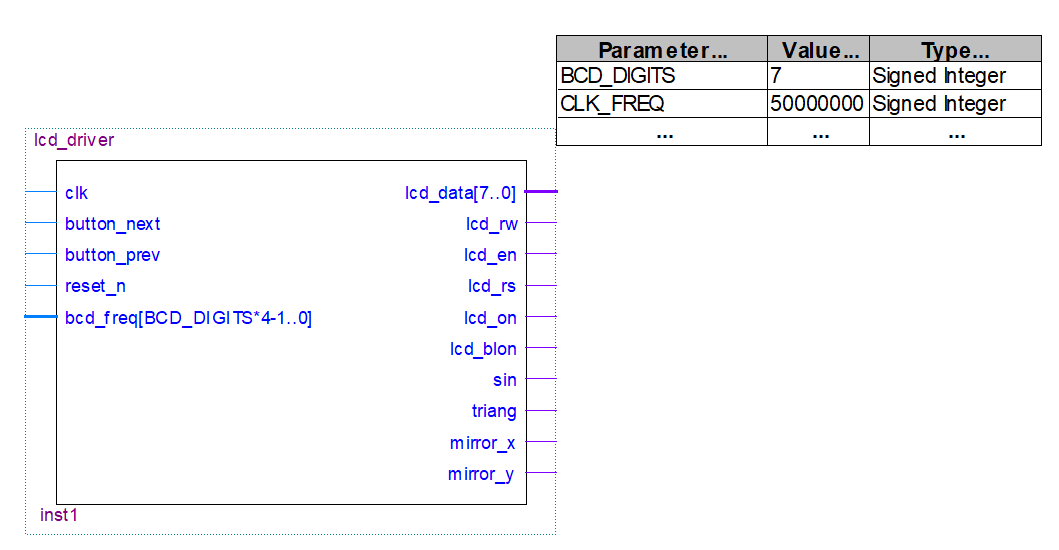
\includegraphics[width=0.8\textwidth]{img/LCD_module_.png}
    \caption{LCD driver module}
    \label{fig:LCD_module}
\end{figure}
\vspace{0.5cm}

\paragraph{I/O interface} \quad \\
The ports used to connect this module to other modules or to the external pins of the FPGA are the following:

\begin{itemize}

    \item \texttt{clk, reset\_n} \\
    are the clock and the synchronous reset pins

    \item \texttt{button\_next, button\_prev} \\
    these are connected to the input buttons used for cycling through each page and so each wave function to display 

    \item \texttt{bcd\_freq} \\
    this input is received from the "Keypad frequency select module" and it is the BCD converted frequency to display on the screen. Each decimal digit to display needs 4 bit to be represented in BCD, so the parameter \texttt{BCD\_DIGITS} is used to instantiate the correct bit value for the digits we want to display

    \item \texttt{lcd\_data} \\
    this is the 8 bit data bus connected to the LCD controller used to write instructions in the IR (instruction register) or the 8 bit ASCII code the DR (data register)

    \item \texttt{lcd\_en} \\
    this pin enable the writing cycle from the data bus to the internal registers of the LCD controller (IR or DR)

    \item \texttt{lcd\_rs} \\
    this pin is used to select the writing on the IR or DR (register select) 

    \item \texttt{lcd\_on} \\
    this pin control the power supply of the LCD and it is always high 

    \item \texttt{lcd\_blon} \\
    this pin control the backlight of the LCD and it is always on 

    \item \texttt{sin ,triang} \\
    these pins are sent to the DDFS module to enable the output of the selected wave function 

    \item \texttt{mirror\_x ,mirror\_y} \\
    these pins are sent to the DDFS module to change the mirroring options of the waveform 
    
\end{itemize}

\paragraph{Parameters} \quad \\
The parameters of this module are:

\begin{itemize}

    \item \texttt{BCD\_DIGITS} \\
    are the number of frequency digit to display on the module.

    \item \texttt{CLK\_FREQ} \\
    is the clock frequency of the clock connected to this module. \\
    Is used to synchronize the timers for the debounce circuits and to respect the timing constrain for the communication with the LCD.
    
\end{itemize}

\paragraph{Verilog code} \quad \\
The LCD module is composed of 2 Synchronous Finite State Machines. One operates to display the name of the selected function in the first row of the screen, while the other continuously displays the selected frequency in the second row of the display when the other FSM is waiting for a button pressure (and release) to change page. \\
To implement two different FSM in the same Verilog code we need to multiplex the shared registers between the two FSM, in our case the registers to be multiplexed are the ones responsible for the LCD driving: \texttt{lcd\_rs}, \texttt{lcd\_data}, \texttt{lcd\_en}. \\
At the end of this combinational always block is present the extrapolation of each BCD number \\ 
(\texttt{bcd\_number}) from the input bit vector (\texttt{bcd\_freq}), using a reverse indexing strategy. 

\vspace{1cm}
\begin{lstlisting}[language=Verilog, caption=Registers multiplexing for FSMs ]
    always @(*) begin
        if( state != WAIT_BUTTON_SHORT && state != WAIT_BUTTON_RELEASE ) begin
            lcd_rs_reg = lut_out[DATA_WIDTH-1];
            lcd_data_reg = lut_out[DATA_WIDTH-2:0];
            lcd_en_reg = lcd_en_cntr;
        end else begin 
            lcd_rs_reg = lcd_rs_freq;
            lcd_data_reg = lcd_data_freq; 		 
            lcd_en_reg = lcd_en_freq;
        end
        //Each BCD (binary coded decimal) digit needs 4 bits
        //number extracted from most significant BCD 
        //to least significant BCD (reverse index)
        bcd_number = bcd_freq[(LAST_BCD_INDEX-(n_index*4))+:BCD_BITS]; 
        if( bcd_number >= 4'd9 ) begin
            bcd_number = 9;
        end
    end
\end{lstlisting}
\vspace{1cm}

\newpage
\noindent
The core of the process to send data to the LCD is here, this mechanism is present in both FSMs, even if in the following piece of code we are going to analyze the first FSM. \\
At the start of the system it is necessary to wait more than 15ms as stated on the datasheet of the \\ \texttt{CFAH1602B-TMC-JP}.
Each new instruction or character writing starts in the \texttt{SETUP} state, the chip enable is set low and a wait time is scheduled, then in the \texttt{WRITE\_DATA} state the enable is set high enabling the sampling of the data to send to the LCD controller, after that the enable is set low again, and a wait for the execution (in the \texttt{WAIT\_EXEC}) is needed before going to the next state, the one responsible to select the next character (or instruction) and eventually the page. 

\noindent
\vspace{1cm}
\begin{lstlisting}[language=Verilog, caption=Sending data to LCD ]
    case (state)
    
        // Wait for more than 15ms at power on 
        POWER_ON: begin
            lcd_en_cntr <= 0;
            counter <= counter + 1'b1;
            if (counter >= wait20ms) begin
                state <= SETUP ;
                counter <= 0;
            end				 
        end
        
        // Setup time wait 
        SETUP: begin
            lcd_en_cntr <= 0;
            counter <= counter + 1'b1;
            if (counter >= wait40us) begin 
                state <= WRITE_DATA;
                counter <= 0;
            end
        end

        // Enable pulse high 
        WRITE_DATA: begin
            lcd_en_cntr <= 1;
            counter <= counter + 1'b1;
            if (counter >= wait1ms) begin 
                state <= WAIT_EXEC; 
                counter <= 0;
            end
        end

        // Wait instruction execution 
        WAIT_EXEC: begin
            lcd_en_cntr <= 0;
            counter <= counter + 1'b1;
            if (counter >= wait2ms) begin 
                char_index <= char_index + 1'b1;	
                state <= PAGE_SELECT; 
                counter <= 0;
            end
        end

        PAGE_SELECT: begin

        .
        .
        .
        
    endcase
\end{lstlisting}
\vspace{1cm}

\newpage

\paragraph{Text LUT instance} \quad \\
A LUT is instantiated with the instructions and ASCII coded characters needed to display the first row of the screen, the one related to the name of the selected waveform and the first two opening pages. \\
This particular LUT is addressable with 2 indexes, one that divides the LUT in pages (\texttt{page\_index}), for a maximum of 32 pages. \\
Each page is composed of 64 memory locations, addressable with the index \texttt{char\_index}. \\
Each address outputs a 9 bit value which has its MSB related to the register select signal (\texttt{lcd\_rs}) to send to the LCD controller, and the remaining 8 bits are related to the data bus (\texttt{lcd\_data}). The resulting dimension of the LUT is:     
\[
    \texttt{TEXT\_LUT\_DIM} = 32\cdot 64\cdot 9 = 2^{11}\cdot 9 = 18432 \texttt{bits} \simeq 18 \texttt{Kb}
\]

\vspace{1cm}
\begin{lstlisting}[language=Verilog, caption=LUT instance ]
    // text LUT instance
    localparam DATA_WIDTH = 9;
    localparam ADDR_WIDTH = 6;
    localparam PAGE_ADDR_WIDTH = 5;
    reg [ADDR_WIDTH-1:0] char_index = 0;
    reg [PAGE_ADDR_WIDTH-1:0] page_index = 0;
    wire [DATA_WIDTH-1:0] lut_out;  
    text_lut #(
        .DATA_WIDTH(DATA_WIDTH),
        .ADDR_WIDTH(ADDR_WIDTH),
        .PAGE_ADDR_WIDTH(PAGE_ADDR_WIDTH)
    ) text_lut_inst (
        .addr(char_index),
        .page(page_index),
        .clk(clk),
        .q(lut_out) 
    );
\end{lstlisting}
\vspace{1cm}

\newpage

\paragraph{First FSM: displaying wave function name} \quad \\
In the \texttt{PAGE\_SELECT} state a sub state strategy is used for each page. \\
The LUT is scanned from the first entry of each page by progressively incrementing \texttt{char\_index} (in the \texttt{WAIT\_EXEC} state), repeating the states cycle \texttt{SETUP}, \texttt{WRITE\_DATA}, \texttt{WAIT\_EXEC}. \\
At each new address, the output of the LUT drives the \texttt{lcd\_rs\_reg} and \texttt{lcd\_data\_reg}. \\
This cycle continues until an @ (hat sign) coded in ASCII is detected, or in case of an error, the end of the page is reached, and an exclusive page signaling the error is displayed. \\
While the first two pages are only used to display information about the project, thus they are displayed for only 2 seconds and automatically shifted, the page starting with the wave function selection capability needs to implement a button press detection and release before displaying a new page.  

\vspace{1cm}
\begin{lstlisting}[language=Verilog, caption= Page selection Sub State Machine ]
    PAGE_SELECT: begin
				
        case(sub_state)

            // DDFS Tonarini Aliberti
            PAGE0: begin
                if (char_index < (2**ADDR_WIDTH)-1) begin
                    if (lcd_data_reg == 8'h40) begin
                        char_index <= 0;
                        page_index <= PAGE1;
                        sub_state <= PAGE1;	
                        state <= WAIT;	
                    end else begin
                        state <= SETUP;
                    end
                end else begin 
                    char_index <= 0; 
                    sub_state <= PAGE_ERROR; 
                end
            end
            
            // Select wave function 
            PAGE1: begin
                if (char_index < 2**ADDR_WIDTH-1) begin
                    if (lcd_data_reg == 8'h40) begin
                        char_index <= 0;
                        page_index <= PAGE2;
                        sub_state <= PAGE2;
                        state <= WAIT;	
                    end else begin
                        state <= SETUP ;
                    end
                end else begin 
                    char_index <= 0; 
                    sub_state <= PAGE_ERROR; 
                end 
            end
            
            .
            .
            .
                
        endcase

    end
\end{lstlisting}
\vspace{1cm}

\newpage
\noindent   
The following code shows the states of the first FSM used to wait for a button to be pressed and released when selecting the wave function. \\
A de-bounce technique is implemented with a 10ms sensing time, and the \texttt{page\_index} is incremented or decremented based on which of the buttons is pressed. 

\vspace{1cm}
\begin{lstlisting}[language=Verilog, caption= Button press and release ]
    WAIT: begin
        counter <= counter + 1'b1;
        if (counter >= wait2s) begin 
            state <= SETUP; 
            counter <= 0;
        end
     
    end

    WAIT_BUTTON_SHORT: begin 			     
        if(button_next == 1'b0 || button_prev == 1'b0) begin 
            btn_counter <= btn_counter + 1'b1;
            if (btn_counter >= wait10ms) begin
                state <= WAIT_BUTTON_RELEASE ;
                btn_counter <= 0;
                    if (button_next == 1'b0) begin
                        btn_pressed <= BTN_NEXT;
                    end else begin
                        btn_pressed <= BTN_PREV;
                    end
            end			
        end else begin
            btn_counter <= 0;
            state <= WAIT_BUTTON_SHORT;
        end					
    end		 
         
    WAIT_BUTTON_RELEASE: begin 			     
        if(button_next == 1'b1 && btn_pressed == BTN_NEXT) begin 
            btn_counter <= btn_counter + 1'b1;
            if (btn_counter >= wait10ms) begin 
                state <= SETUP;
                btn_counter <= 0;								
                if (page_index >= PAGE_FIRST && page_index < PAGE_LAST) begin
                    page_index <= page_index + 1'b1;
                end else if ( page_index == PAGE_LAST ) begin
                    page_index <= PAGE_FIRST;
                end							
            end		
        end else if (button_prev == 1'b1 && btn_pressed == BTN_PREV) begin
            btn_counter <= btn_counter + 1'b1;
            if (btn_counter >= wait10ms) begin 
                state <= SETUP;
                btn_counter <= 0;								
                if (page_index > PAGE_FIRST && page_index <= PAGE_LAST) begin
                    page_index <= page_index - 1'b1;
                end else if ( page_index == PAGE_FIRST ) begin
                    page_index <= PAGE_LAST;
                end							
            end
        end else begin
            state <= WAIT_BUTTON_RELEASE;
            btn_counter <= 0;
        end				
    end
\end{lstlisting}
\vspace{1cm}

\paragraph{Second FSM: displaying wave function frequency} \quad \\
This FSM is used to show the frequency of the selected wave function on the second row of the LCD. \\
It starts cycling through the states when the first FSM is waiting for a button to be pressed or released. \\
The \texttt{DIGIT\_SELECT} state provides the ASCII code, calculated from the BCD number received as input, to the \texttt{lcd\_data\_freq} register to display each digit on the screen. \\
When all digits are correctly displayed the \texttt{HZ\_DISPLAY} state print on the screen " Hz" at the end of the frequency value. \\
It is important to note that, again, like the first FSM, to display each character a cycle of the writing states needs to be executed (\texttt{SETUP}, \texttt{WRITE\_DATA}, \texttt{WAIT\_EXEC}).

\vspace{1cm}
\begin{lstlisting}[language=Verilog, caption= Digit selection and Hz display ]
    DIGIT_SELECT: begin
        lcd_rs_freq <= 1'b1;
        lcd_data_freq <= bcd_number + 8'h30;
        n_index <= n_index + 1'b1;
        if ( n_index >= BCD_DIGITS ) begin
            state_f <= HZ_DISPLAY;
        end else begin
            state_f <= SETUP;
        end		 						
    end
         
    HZ_DISPLAY: begin
        case(sub_state_f)
            0: begin
                lcd_data_freq <= 8'h20;
                sub_state_f <= sub_state_f + 1'b1;
                state_f <= SETUP;
            end
            1: begin
                lcd_data_freq <= 8'h48;
                sub_state_f <= sub_state_f + 1'b1;
                state_f <= SETUP;
            end
            2: begin
                lcd_data_freq <= 8'h7A;
                sub_state_f <= sub_state_f + 1'b1;
                state_f <= SETUP;
            end	
            3: begin
                sub_state_f <= 0;
                state_f <= CHECK_AND_WAIT;
            end	
        endcase
    end
\end{lstlisting}
\vspace{1cm}



\newpage

\subsection{Clock distribution}

The project is composed of different modules synchronized with a common clock source. \\
The main clock lines are the external \(50MHz\) clock and the PLL multiplied \(70MHz\) clock. \\
These two clocks have the same phase because the internal FPGA PLL has been configured to make this possible. \\
The three synchronized main modules are 

\begin{itemize}
    \item \texttt{keypad\_freq\_sel\_module}
    \item \texttt{ddfs}
    \item \texttt{lcd\_driver}
\end{itemize}

\noindent
The \texttt{keypad\_freq\_sel\_module} has an internal clock enable to reduce the throughput (to scan the keypad more slowly) and to communicate with the other modules using the same clock source. \\
The \texttt{ddfs} module has an internal frequency clock divider, programmable through the external pins of the module. \\
The problem with using an internal frequency divider is that the divided clock is shifted by a time \(t_{co}\) (clock-to-output time) of the flip-flop that generates it, and this can lead to setup and hold time violations. \\
The output of the module goes only to the DAC, and the DAC clock is connected to the output of the frequency divider; the problem is that the \texttt{f\_w} and the \texttt{mirror\_x, mirror\_y} inputs are sampled with the divided clock of the frequency divider. \\
The delay is not a problem, because the \texttt{f\_w} and the \texttt{mirror\_x, mirror\_y} inputs remain constant for all the time that the output waves are shown, which is usually seconds or minutes; therefore, even if for some clock cycles the data is not sampled correctly, after some time the situation is fixed automatically. \\
The main problem is metastability due to hold or setup time violations.\\
To analyze this system, the output of the frequency divider is considered by the timing analyzer as a fixed clock with the maximum clock frequency (worst-case analysis), and it verifies whether the setup and hold slack is greater than zero.\\
The issue is that the timing analyzer considers the signal to be in phase with the original clock, which is not the case. \\
Therefore, to protect the system from metastability, the use of a latch chain to protect the \texttt{f\_w} and the \texttt{mirror\_x, mirror\_y} inputs is suggested. \\
Other solutions has been analyzed in \autoref{sec:conclusions}.

\noindent

    \newpage
    \section{Test-plan}
\label{sec:test-plan}

\subsection{Functional verification}

The functional verification of a verilog module is the process of checking that the module behaves exactly as intended according to its specification. \\
It is typically done through simulation using testbenches that apply input signals and observe outputs over time. \\
The goal is to find logical and design errors before synthesis.

\subsubsection{DDFS module}

The test-plan for the DDFS module consist on checking every type of output waveform with different \texttt{f\_w} and \texttt{freq\_cntrl} values.

\paragraph{Testbench} \quad \\
The testbench applies every combination of the pins \texttt{sin, triang, mirror\_x, mirror\_y} for \(50000\) clock cycles with \(\texttt{f\_w} = 0\) and \(\texttt{freq\_cntrl} = 0\). \\
Then, the value of \(\texttt{f\_w}\) is changed to observe how the frequency and the accuracy of the output wave vary with this parameter.

\vspace{1cm}
\begin{lstlisting}[language=Verilog, caption=DDFS testbench ]
    //testing every combination of input signals
    for(i=0; i<4'b1111;i=i+1) begin
        #(CLOCK_PERIOD*50000)
        {mirror_x, mirror_y, sin, triang} = i;
    end
    
    //apply sine wave
    #(CLOCK_PERIOD*50000)
    {sin, triang, mirror_x, mirror_y} = 4'b1111;		//testing sin priority
    
    //changing frequency word
    for(i=0; i<7'b1111111; i=i+10) begin
        #(CLOCK_PERIOD*50000)
        fw = i;
    end
\end{lstlisting}
\vspace{1cm}

\noindent
The \texttt{freq\_cntrl} parameter variation has been tested in the frequency divider testbench. \\
In the frequency divider testbench, the clock output of the frequency divider module has been analyzed as the \texttt{freq\_cntrl} parameter value is varied.

\newpage
\paragraph{Wave analysis} \quad \\
To analyze the output waveform of the DDFS module, it has been represented both as an unsigned value and in analog form. \\
This allows the digital numbers to be visualized as an analog waveform. \\
The first thing to observe from the testbench is the output waveform for every combination of the input values (while keeping the same value of \texttt{f\_w}).

\vspace{0.5cm}
\begin{figure}[h!]
    \centering
    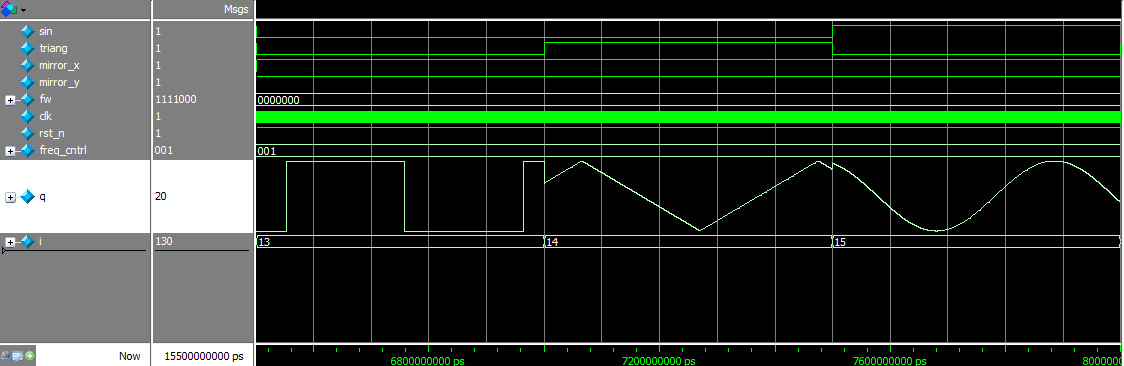
\includegraphics[width=\textwidth]{img/DDFS_outpu_wave.jpg}
    \caption{DDFS testbench output wave}
    \label{fig:DDFS_output_wave}
\end{figure}
\vspace{0.5cm}

\noindent
In \autoref{fig:DDFS_output_wave} are shown the three main waveform with both mirroring effect enabled. \\
The second thing that can be analyzed from the testbench is the variation of the output frequency corresponding to a swing of \texttt{f\_w}.

\vspace{0.5cm}
\begin{figure}[h!]
    \centering
    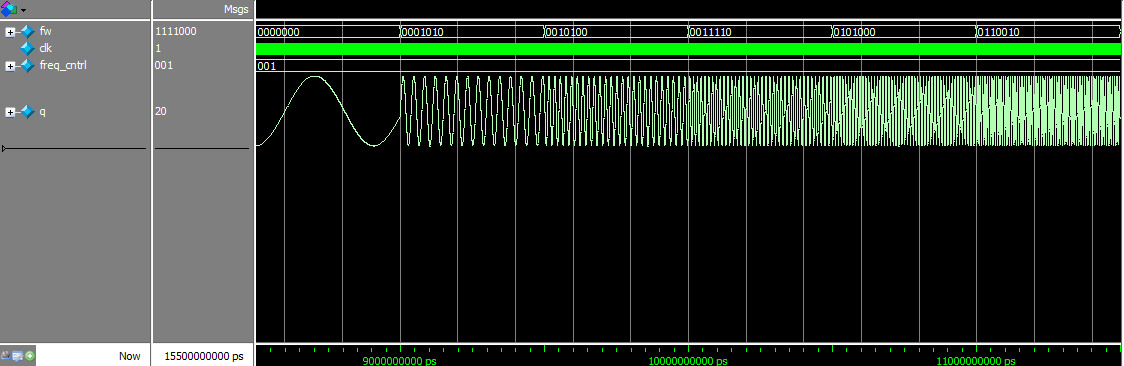
\includegraphics[width=\textwidth]{img/fw_variation_DDFS.jpg}
    \caption{DDFS sine-wave frequency swing}
    \label{fig:fw_variation_DDFS}
\end{figure}
\vspace{0.5cm}
\begin{figure}[h!]
    \centering
    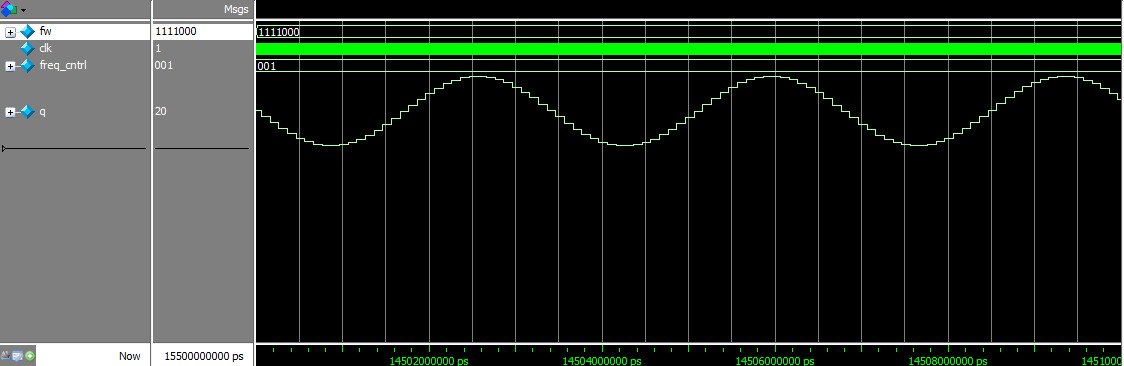
\includegraphics[width=\textwidth]{img/smallest_fw_wave_DDFS.jpg}
    \caption{DDFS sine-wave with biggest value of \texttt{f\_w}}
    \label{fig:smallest_fw_wave_DDFS}
\end{figure}
\vspace{0.5cm}

\noindent
For the frequency divider, only the output frequencies \(\frac{f_{clk}}{2}\), \(\frac{f_{clk}}{10}\), \(\frac{f_{clk}}{100}\), and \(\frac{f_{clk}}{1000}\) were tested, since the other divisions are too large to be simulated.

\vspace{0.5cm}
\begin{figure}[h!]
    \centering
    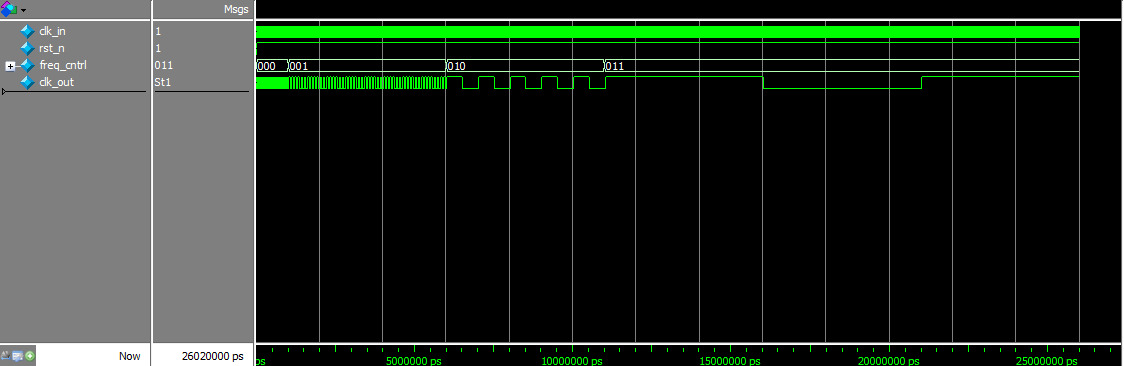
\includegraphics[width=\textwidth]{img/freq_div_DDFS.jpg}
    \caption{DDFS divided frequency from frequency divider}
    \label{fig:freq_div_DDFS}
\end{figure}
\vspace{0.5cm}

\newpage

\subsubsection{Keypad frequency select module}
The test procedure for this module is divided into different parts:  
the test of the keypad module, the test of the frequency converter module, and the test of the modules connected together. \\
To simulate the behavior of the 4×4 matrix keypad (used for the keypad module and for the keypad frequency selection module), a dedicated module has been implemented. \\
This module is controlled via an input bus and simulates the electrical connection between the corresponding columns and rows.

\vspace{1cm}
\begin{lstlisting}[language=Verilog, caption=4x4 keypad simulator module  ]
    module keypad_4x4
    (
        // ---- KEYPAD PINS ---- //
        input [3:0] column,
        output reg [3:0] row,
        
        // ---- BUTTON PINS ---- //
        input [3:0] button,
        input button_pressed
    );
    
        integer i;
        always @(*) begin		
            //assign button value
            if(button_pressed == 1)
                for(i=0; i<4; i=i+1) begin
                    if(i == button/4)
                        row[i] = column[button%4];
                    else
                        row[i] = 1;
                end
            else
                row = 4'b1111;
        end
    
    endmodule
\end{lstlisting}
\vspace{1cm}

\paragraph{Testbench} \quad \\
To test the keypad module, the press of a different keypad button was simulated every \(100ns\), and the values of the \texttt{out\_keys} and \texttt{data\_valid} outputs were read.

\vspace{1cm}
\begin{lstlisting}[language=Verilog, caption=Keypad module testbench  ]
    //none button pressed
    button_pressed = 0;
    
    for(i=0; i<=4'b1111; i=i+1) begin
        //press a button
        #100
        button_pressed = 1;
        button = i;		
    end
    
    //none button pressed
    #100 button_pressed = 0;
\end{lstlisting}
\vspace{1cm}

\noindent
To test the DDFS frequency converter module, the value of the module input frequency was increased from \(0\) to \texttt{MAX\_FREQ}, which was set to \(1MHz\), with a \texttt{CLK\_FREQ} of \(70MHz\). \\
Due to the large range of frequency values, the increment step was set to \(100\).

\vspace{1cm}
\begin{lstlisting}[language=Verilog, caption=DDFS converter module testbench  ]
    for(i=0; i<=MAX_FREQ; i=i+100) begin
        #10 freq = i;
    end
\end{lstlisting}
\vspace{1cm}

\noindent
To test the accuracy of the module with different clock scaling factors, the output waveform frequency was also calculated using the \texttt{f\_w} and \texttt{freq\_cntrl} values processed by the module. \\
Then, the \texttt{delta\_freq} was calculated as the difference between the ideal frequency (the input of the DDFS converter module) and the real frequency (calculated from the output of the DDFS converter module).

\vspace{1cm}
\begin{lstlisting}[language=Verilog, caption=Delta frequency calculation  ]
    reg [63:0] divided_clock;
    always @(*) begin
        case(freq_control)
            
            //select the correct divided_clock output
            3'd0: divided_clock = CLK_FREQ/2;
            3'd1: divided_clock = CLK_FREQ/10;
            3'd2: divided_clock = CLK_FREQ/100;
            3'd3: divided_clock = CLK_FREQ/1000;
            3'd4: divided_clock = CLK_FREQ/10000;
            3'd5: divided_clock = CLK_FREQ/100000;
            3'd6: divided_clock = CLK_FREQ/1000000;
            
            default: begin
                //error stop simulation
                $error("ERROR: frequency divider value out of range");
                $stop;
            end
                
        endcase
    end
    
    assign @(*) begin
    
        if(mirror_x == 0 && mirror_y == 0) begin
            freq_calculated = ((fw+1)*divided_clock)/1024;
        end
        else if(mirror_x == 0 || mirror_y == 0) begin
            freq_calculated = 2*((fw+1)*divided_clock)/1024;
        end
        else begin
            freq_calculated = 4*((fw+1)*divided_clock)/1024;
        end
    
    end
    
    assign delta_freq = freq - freq_calculated;
\end{lstlisting}
\vspace{1cm}

\newpage
\paragraph{Wave analysis} \quad \\
From the keypad module testbench, it is possible to observe the column enabling cycle and the row reading cycle.

\vspace{0.5cm}
\begin{figure}[h!]
    \centering
    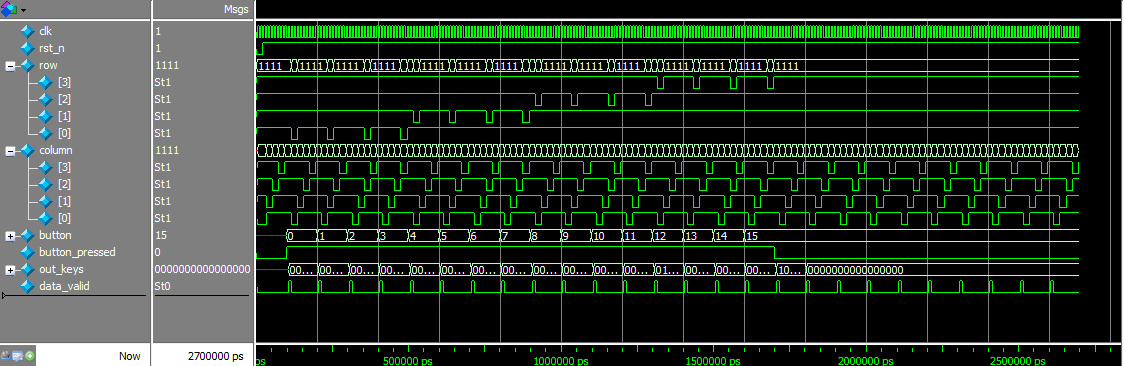
\includegraphics[width=\textwidth]{img/keypad_module_waveform.jpg}
    \caption{Keypad module waveform of scan cycles}
    \label{fig:keypad_module_waveform}
\end{figure}
\vspace{0.5cm}

\noindent
Enabling a column and reading the corresponding rows takes two clock cycles. \\
The output data (rows and column of the button pressed) is sampled and stored into a buffer and at the end of the scanning cycle the value of the buffer is stored into the output vector.

\vspace{0.5cm}
\begin{figure}[h!]
    \centering
    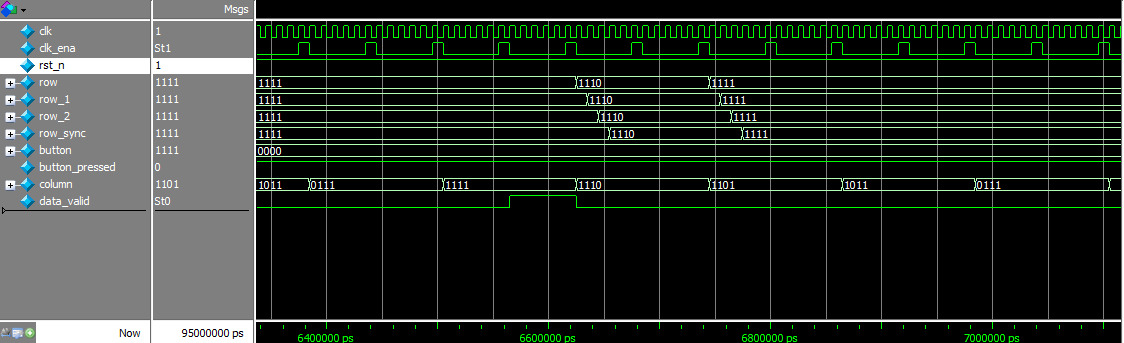
\includegraphics[width=\textwidth]{img/keypad_waveform_detail.jpg}
    \caption{Sampling data of keypad module}
    \label{fig:keypad_waveform_detail}
\end{figure}
\vspace{0.5cm}

\noindent
In \autoref{fig:keypad_waveform_detail} we can see that the row inputs pass through three flip-flops to reduce metastability problems, but this does not cause trouble, because the clock enable rises after \texttt{row\_sync} has stabilized.

\newpage
\noindent
By analyzing the DDFS converter module testbench, we can observe the variation of \texttt{delta\_freq} for a sweep of the input frequency from \(0\,\text{Hz}\) to \(1\,\text{MHz}\), and calculate the maximum absolute (and relative) frequency error for each frequency division (from the frequency divider).

\vspace{0.5cm}
\begin{figure}[h!]
    \centering
    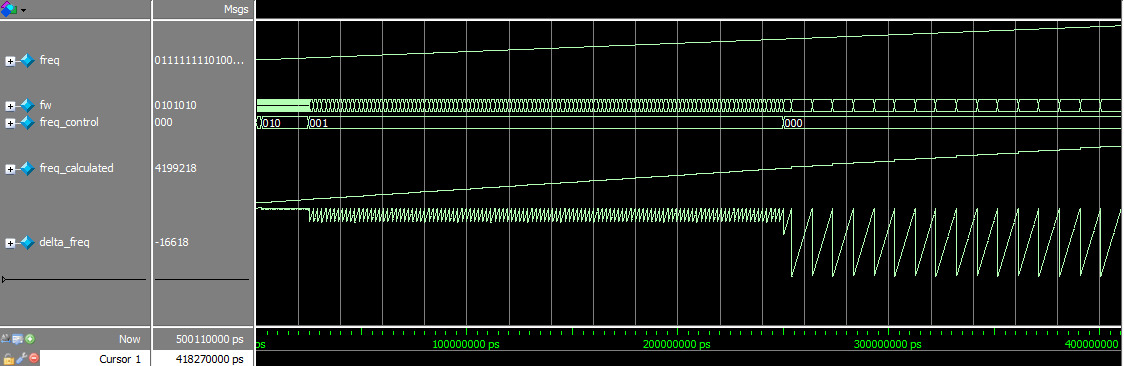
\includegraphics[width=\textwidth]{img/DDFS_freq_wave.jpg}
    \caption{Testbench output of DDFS converter module}
    \label{fig:DDFS_freq_wave}
\end{figure}
\vspace{0.5cm}

\noindent
As we can see in \autoref{fig:DDFS_freq_wave}, the absolute value of \texttt{delta\_freq} is lower than a value that depends on the frequency control calculated by the module. \\
The \texttt{delta\_freq} value is equal to the absolute frequency error.


\begin{itemize}

    \item \(\texttt{freq\_control} = 000\) \\
    \(
        \left|\varepsilon_{a}\right| = \left| f_{in} - f_{measured} \right| < 33000Hz \implies 
        \left|\varepsilon_{r}\right| = \left| \frac{ f_{in} - f_{measured} }{f_{in}} \right| < \left| \frac{ max(\varepsilon_{a}) }{min(f_{in})} \right| \simeq 3.8 \%
    \)
    
    \item \(\texttt{freq\_control} = 001\) \\
    \(
        \left|\varepsilon_{a}\right| = \left| f_{in} - f_{measured} \right| < 6500Hz \implies 
        \left|\varepsilon_{r}\right| = \left| \frac{ f_{in} - f_{measured} }{f_{in}} \right| < \left| \frac{ max(\varepsilon_{a}) }{min(f_{in})} \right| \simeq 7.2 \%
    \)
    
    \item \(\texttt{freq\_control} = 010\) \\
    \(
        \left|\varepsilon_{a}\right| = \left| f_{in} - f_{measured} \right| < 650Hz \implies 
        \left|\varepsilon_{r}\right| = \left| \frac{ f_{in} - f_{measured} }{f_{in}} \right| < \left| \frac{ max(\varepsilon_{a}) }{min(f_{in})} \right| \simeq 7.0 \%
    \)
    
    \item \(\texttt{freq\_control} = 011\) \\
    \(
        \left|\varepsilon_{a}\right| = \left| f_{in} - f_{measured} \right| < 65Hz \implies 
        \left|\varepsilon_{r}\right| = \left| \frac{ f_{in} - f_{measured} }{f_{in}} \right| < \left| \frac{ max(\varepsilon_{a}) }{min(f_{in})} \right| \simeq 7.1 \%
    \)

    \item \(\texttt{freq\_control} = 100\) \\
    \(
        \left|\varepsilon_{a}\right| = \left| f_{in} - f_{measured} \right| < 6Hz \implies 
        \left|\varepsilon_{r}\right| = \left| \frac{ f_{in} - f_{measured} }{f_{in}} \right| < \left| \frac{ max(\varepsilon_{a}) }{min(f_{in})} \right| \simeq 6.7 \%
    \)

    \item \(\texttt{freq\_control} = 101\) \\
    \(
        \left|\varepsilon_{a}\right| = \left| f_{in} - f_{measured} \right| < 1Hz \implies 
        \left|\varepsilon_{r}\right| = \left| \frac{ f_{in} - f_{measured} }{f_{in}} \right| < \left| \frac{ max(\varepsilon_{a}) }{min(f_{in})} \right| \simeq 0 \%
    \)

    \item \(\texttt{freq\_control} = 110\) \\
    \(
        \left|\varepsilon_{a}\right| = \left| f_{in} - f_{measured} \right| = 0Hz \implies 
        \left|\varepsilon_{r}\right| = \left| \frac{ f_{in} - f_{measured} }{f_{in}} \right| = 0\%
    \)
    
\end{itemize}

\newpage

\subsubsection{LCD module}
We want to test the correct states change of the two FSM of the LCD module. 

\paragraph{Testbench} \quad \\
Only for simulation purposes the delays needed to drive the LCD are reduced to a fixed value of 40 ns, this way it is simpler to test the module with Modelsim. To solve this scope a testing Verilog file is created (\texttt{lcd\_driver\_test.v})

\vspace{0.5cm}
\begin{lstlisting}[language=Verilog, caption=LCD module testbench  ]
    initial begin
        reset_n = 1'b0;
        button_next = 1'b1;
        button_prev = 1'b1;
        bcd_freq = 28'hFFFFFFF;
        
        #(CLK_PERIOD*2)	  
        reset_n = 1'b1;
        
        #(CLK_PERIOD*2000)
        button_next = 1'b0;
        
        #(CLK_PERIOD*10)
        button_next = 1'b1;
        
        #(CLK_PERIOD*1000)
        button_next = 1'b0;
        
        #(CLK_PERIOD*10)
        button_next = 1'b1;
        
        #(CLK_PERIOD*1000)
        button_prev = 1'b0;
        
        #(CLK_PERIOD*10)
        button_prev = 1'b1;
            
        #(CLK_PERIOD*1000)
        // Finish simulation
        $stop;
    end
\end{lstlisting}
\vspace{1cm}

\newpage

\paragraph{Wave analysis} \quad \\
The simulation starts with a reset and after that the \texttt{POWER\_ON} state is enabled, followed by the first writing cycle to the LCD. As we can see, at first, in the \texttt{lcd\_data} register is stored the first instruction present in the LUT to send to the LCD (hex38, initializing the function set), then when the first writing cycle is completed the next instruction is read from the LUT and loaded in the \texttt{lcd\_data} register. 

\vspace{0.5cm}
\begin{figure}[h!]
    \centering
    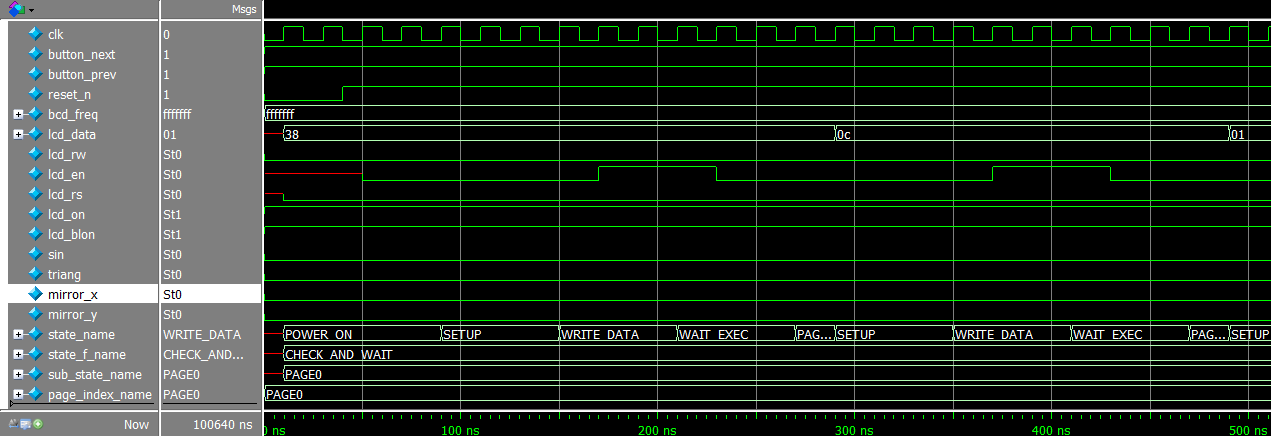
\includegraphics[width=\textwidth]{img/LCD_module_wave1.png}
    \caption{LCD power on}
    \label{fig:LCD_module_wave1}
\end{figure}
\vspace{0.5cm}

\noindent
After sending the first instruction to initialize the LCD we can start to send ASCII characters by setting the register select flag to 1. In \autoref{fig:LCD_module_wave2} we see the ASCII coded characters that are written to the DDRAM of the LCD, each in sequence with a writing cycle. 

\vspace{0.5cm}
\begin{figure}[h!]
    \centering
    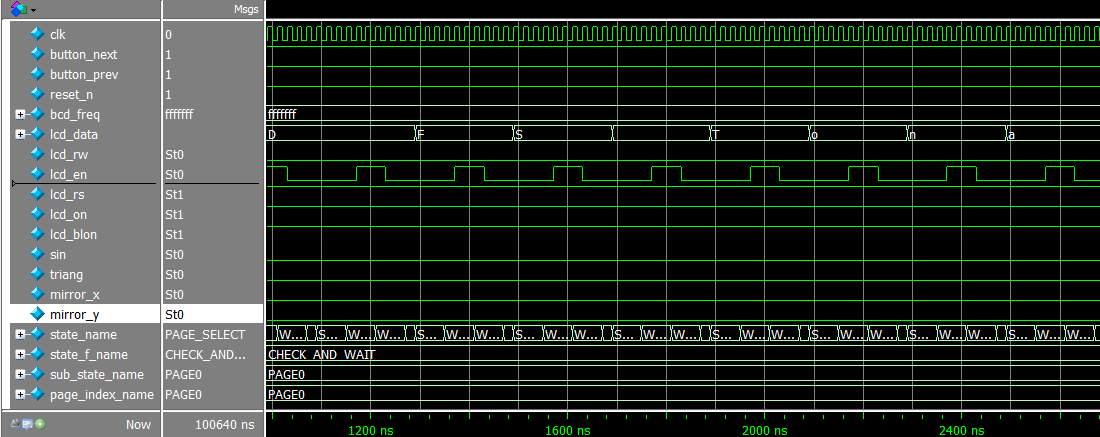
\includegraphics[width=\textwidth]{img/LCD_module_wave2.png}
    \caption{Displaying characters}
    \label{fig:LCD_module_wave2}
\end{figure}
\vspace{0.5cm}

\newpage

\noindent
When a page is completely displayed the first FSM enters the \texttt{WAIT\_BUTTON\_SHORT} state, waiting for the button to be pressed and released. At this point the second FSM is activated, displaying the frequency digits received as BCD input vector in the second row of the display (\autoref{fig:LCD_module_wave3}).  

\vspace{0.5cm}
\begin{figure}[h!]
    \centering
    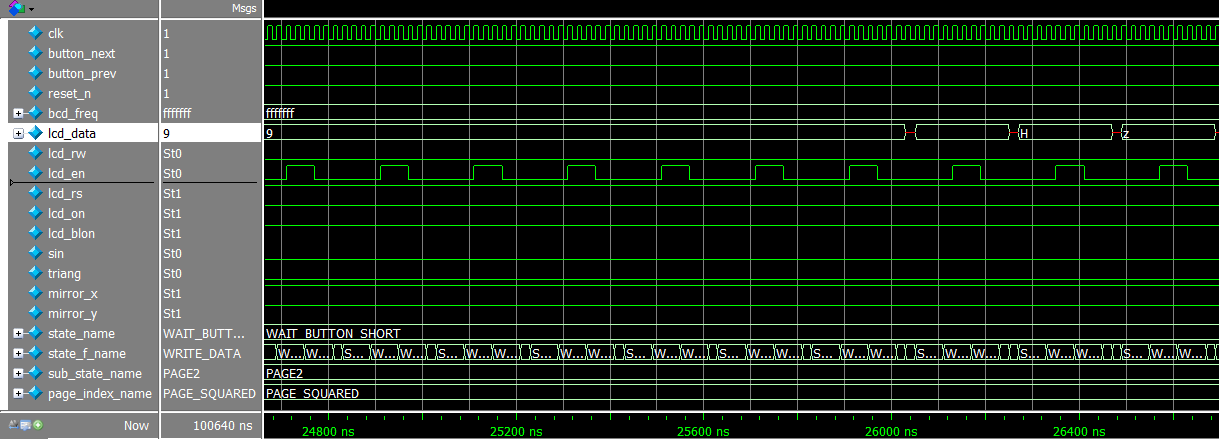
\includegraphics[width=\textwidth]{img/LCD_module_wave3.png}
    \caption{Displaying frequency digits}
    \label{fig:LCD_module_wave3}
\end{figure}
\vspace{0.5cm}

\noindent
In the example in \autoref{fig:LCD_module_wave4} the button is pressed to change the wave function to display, changing from squared wave to triangular wave, the output \texttt{triang} is enabled to signal the new waveform to the DDFS module. Since a new page with new characters needs to be displayed, a new writing cycle of the first FSM starts, the second FSM starts waiting until the first FSM has completed the job (entering the \texttt{WAIT\_BUTTON\_SHORT} state again).  

\vspace{0.5cm}
\begin{figure}[h!]
    \centering
    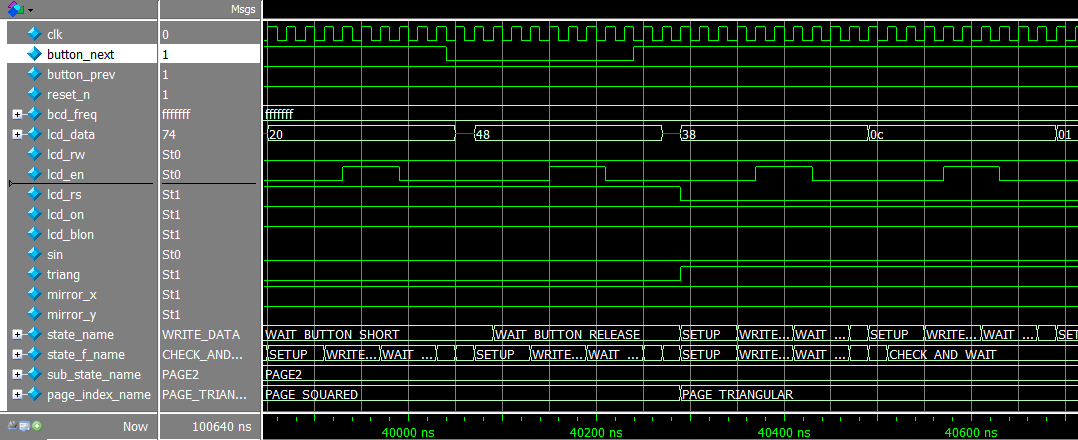
\includegraphics[width=\textwidth]{img/LCD_module_wave4.png}
    \caption{Changing wave function}
    \label{fig:LCD_module_wave4}
\end{figure}
\vspace{0.5cm}

\newpage

\subsection{On-board module testing}
To verify that each module works properly on the board, each module has been tested individually on the board, using the keys, buttons, and LEDs present on the \textbf{Altera DE2 development board}.

\subsubsection{DDFS module}

\vspace{0.5cm}
\begin{figure}[h!]
    \centering
    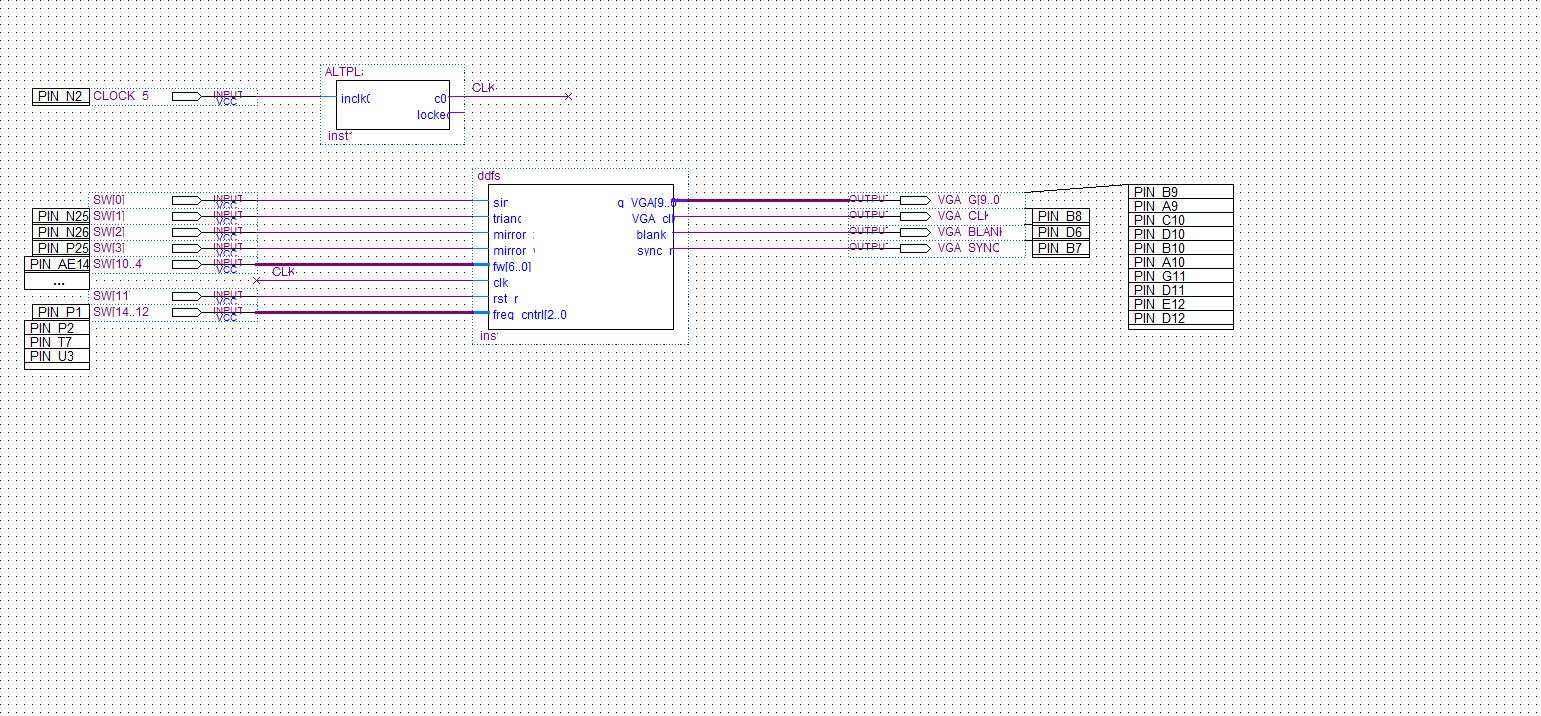
\includegraphics[width=\textwidth]{img/DDFS_onboard_test.jpg}
    \caption{DDFS onboard test schematic}
    \label{fig:DDFS_onboard_test}
\end{figure}
\vspace{0.5cm}

\noindent
As we can see from \autoref{fig:DDFS_onboard_test}, the module inputs have been connected to the keys on the board.\\
The output has been connected to the VGA DAC inputs.\\
The input \(50MHz\) clock source from the board passes through the internal PLL of the FPGA and becomes a \(70MHz\) clock signal. \\
The oscilloscope can be connected to the green channel of the VGA port to monitor the analog output signal of the waveform generator and verify that the output matches the module's input.

\newpage

\subsubsection{Keypad frequency select module}

\vspace{0.5cm}
\begin{figure}[h!]
    \centering
    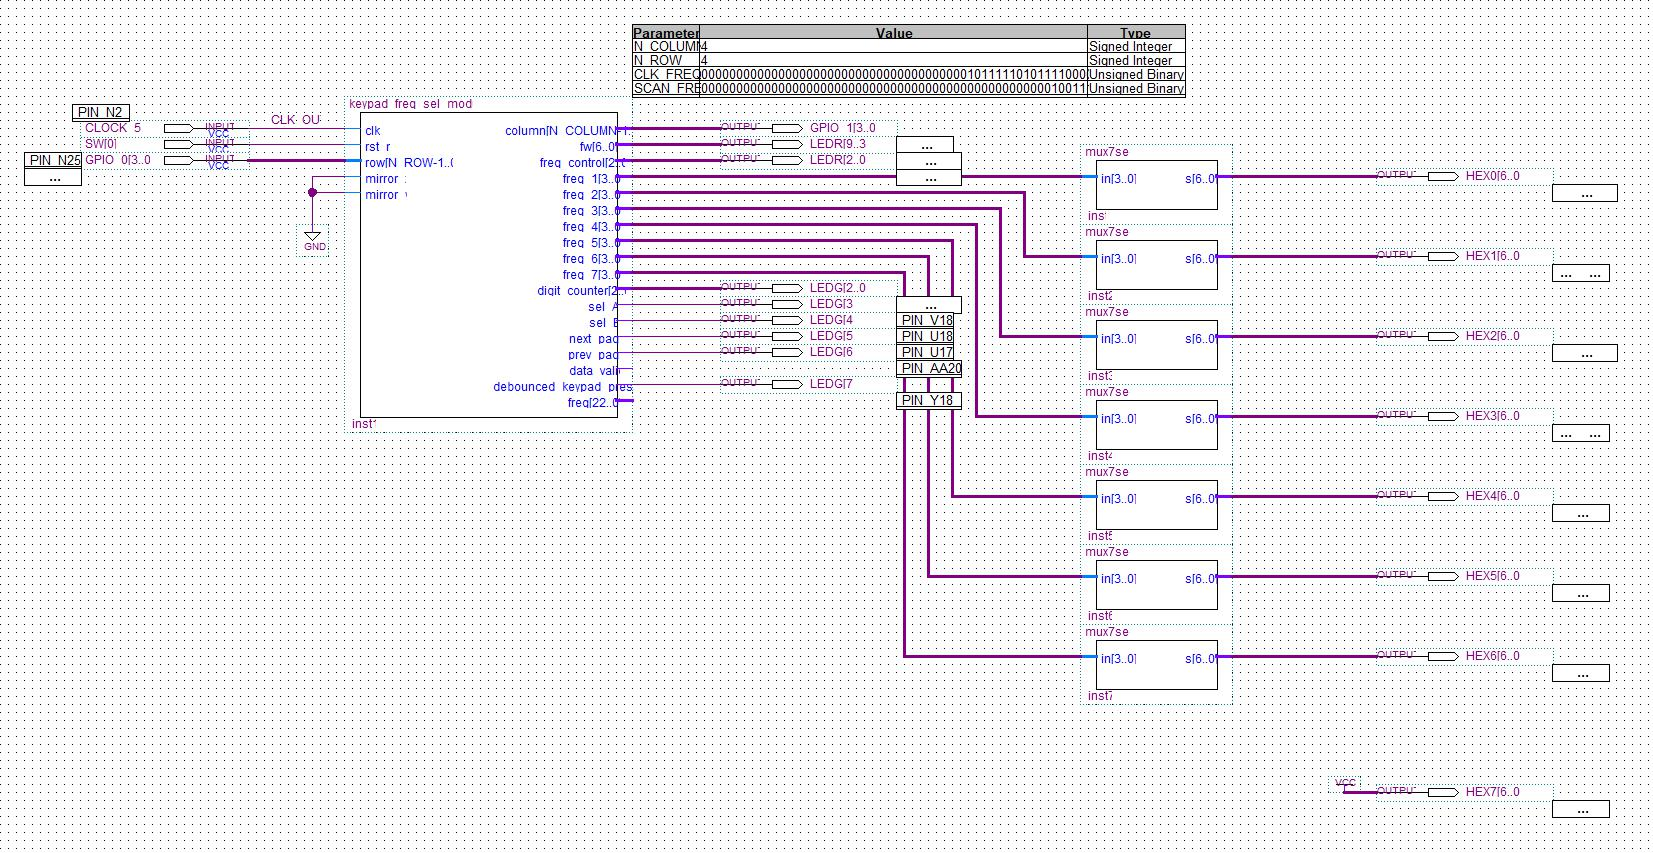
\includegraphics[width=\textwidth]{img/keypad_freq_sel_onboard_test.jpg}
    \caption{keypad frequency select onboard test schematic}
    \label{fig:keypad_freq_sel_onboard_test}
\end{figure}
\vspace{0.5cm}

\noindent
The pins of the keypad have been connected to the GPIO of the board, and the input pins must be configured as input pull-up. \\
The output of the module has been connected, through a BCD-to-7-segment display converter module, to the 7-segment displays on the board, to control the digit shift and the selection of the output signal. \\
The clock source comes from the oscillator on the board but the module work with a clock enable signal, to match the frequency scan value (an external parameter). \\
The other control pins for the DDFS module are connected to the remaining LEDs on the board.

\newpage

\subsubsection{LCD module}

\vspace{0.5cm}
\begin{figure}[h!]
    \centering
    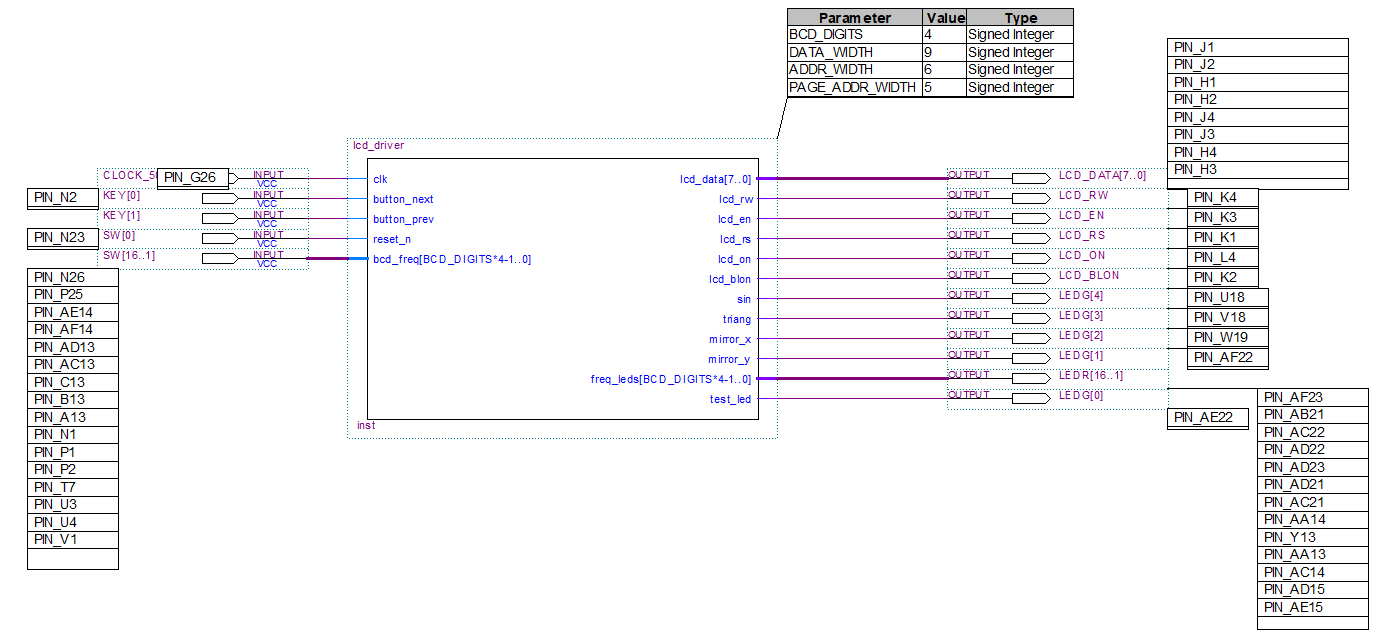
\includegraphics[width=\textwidth]{img/LCD_module_assignment.png}
    \caption{LCD module onboard test schematic}
    \label{fig:LCD_module_assignment}
\end{figure}
\vspace{0.5cm}

\noindent
In the testing phase of the LCD module it has been useful to connect the inputs of the \texttt{bcd\_freq} vector to 16 switches of the board to display at least 4 variable digits (4 switches for each BCD digit), the button for the next and previous page were connected to two physical buttons of the board, and LEDs were used to show the outputs (sin, triang, mirror\_x, mirror\_y) and to test the buttons and switch activation (test\_led, freq\_leds). 

\newpage
\subsubsection{Physical test of the entire design}
In this section some examples and capabilities of the final design are shown.

\vspace{0.5cm}
\begin{figure}[h!]
    \centering
    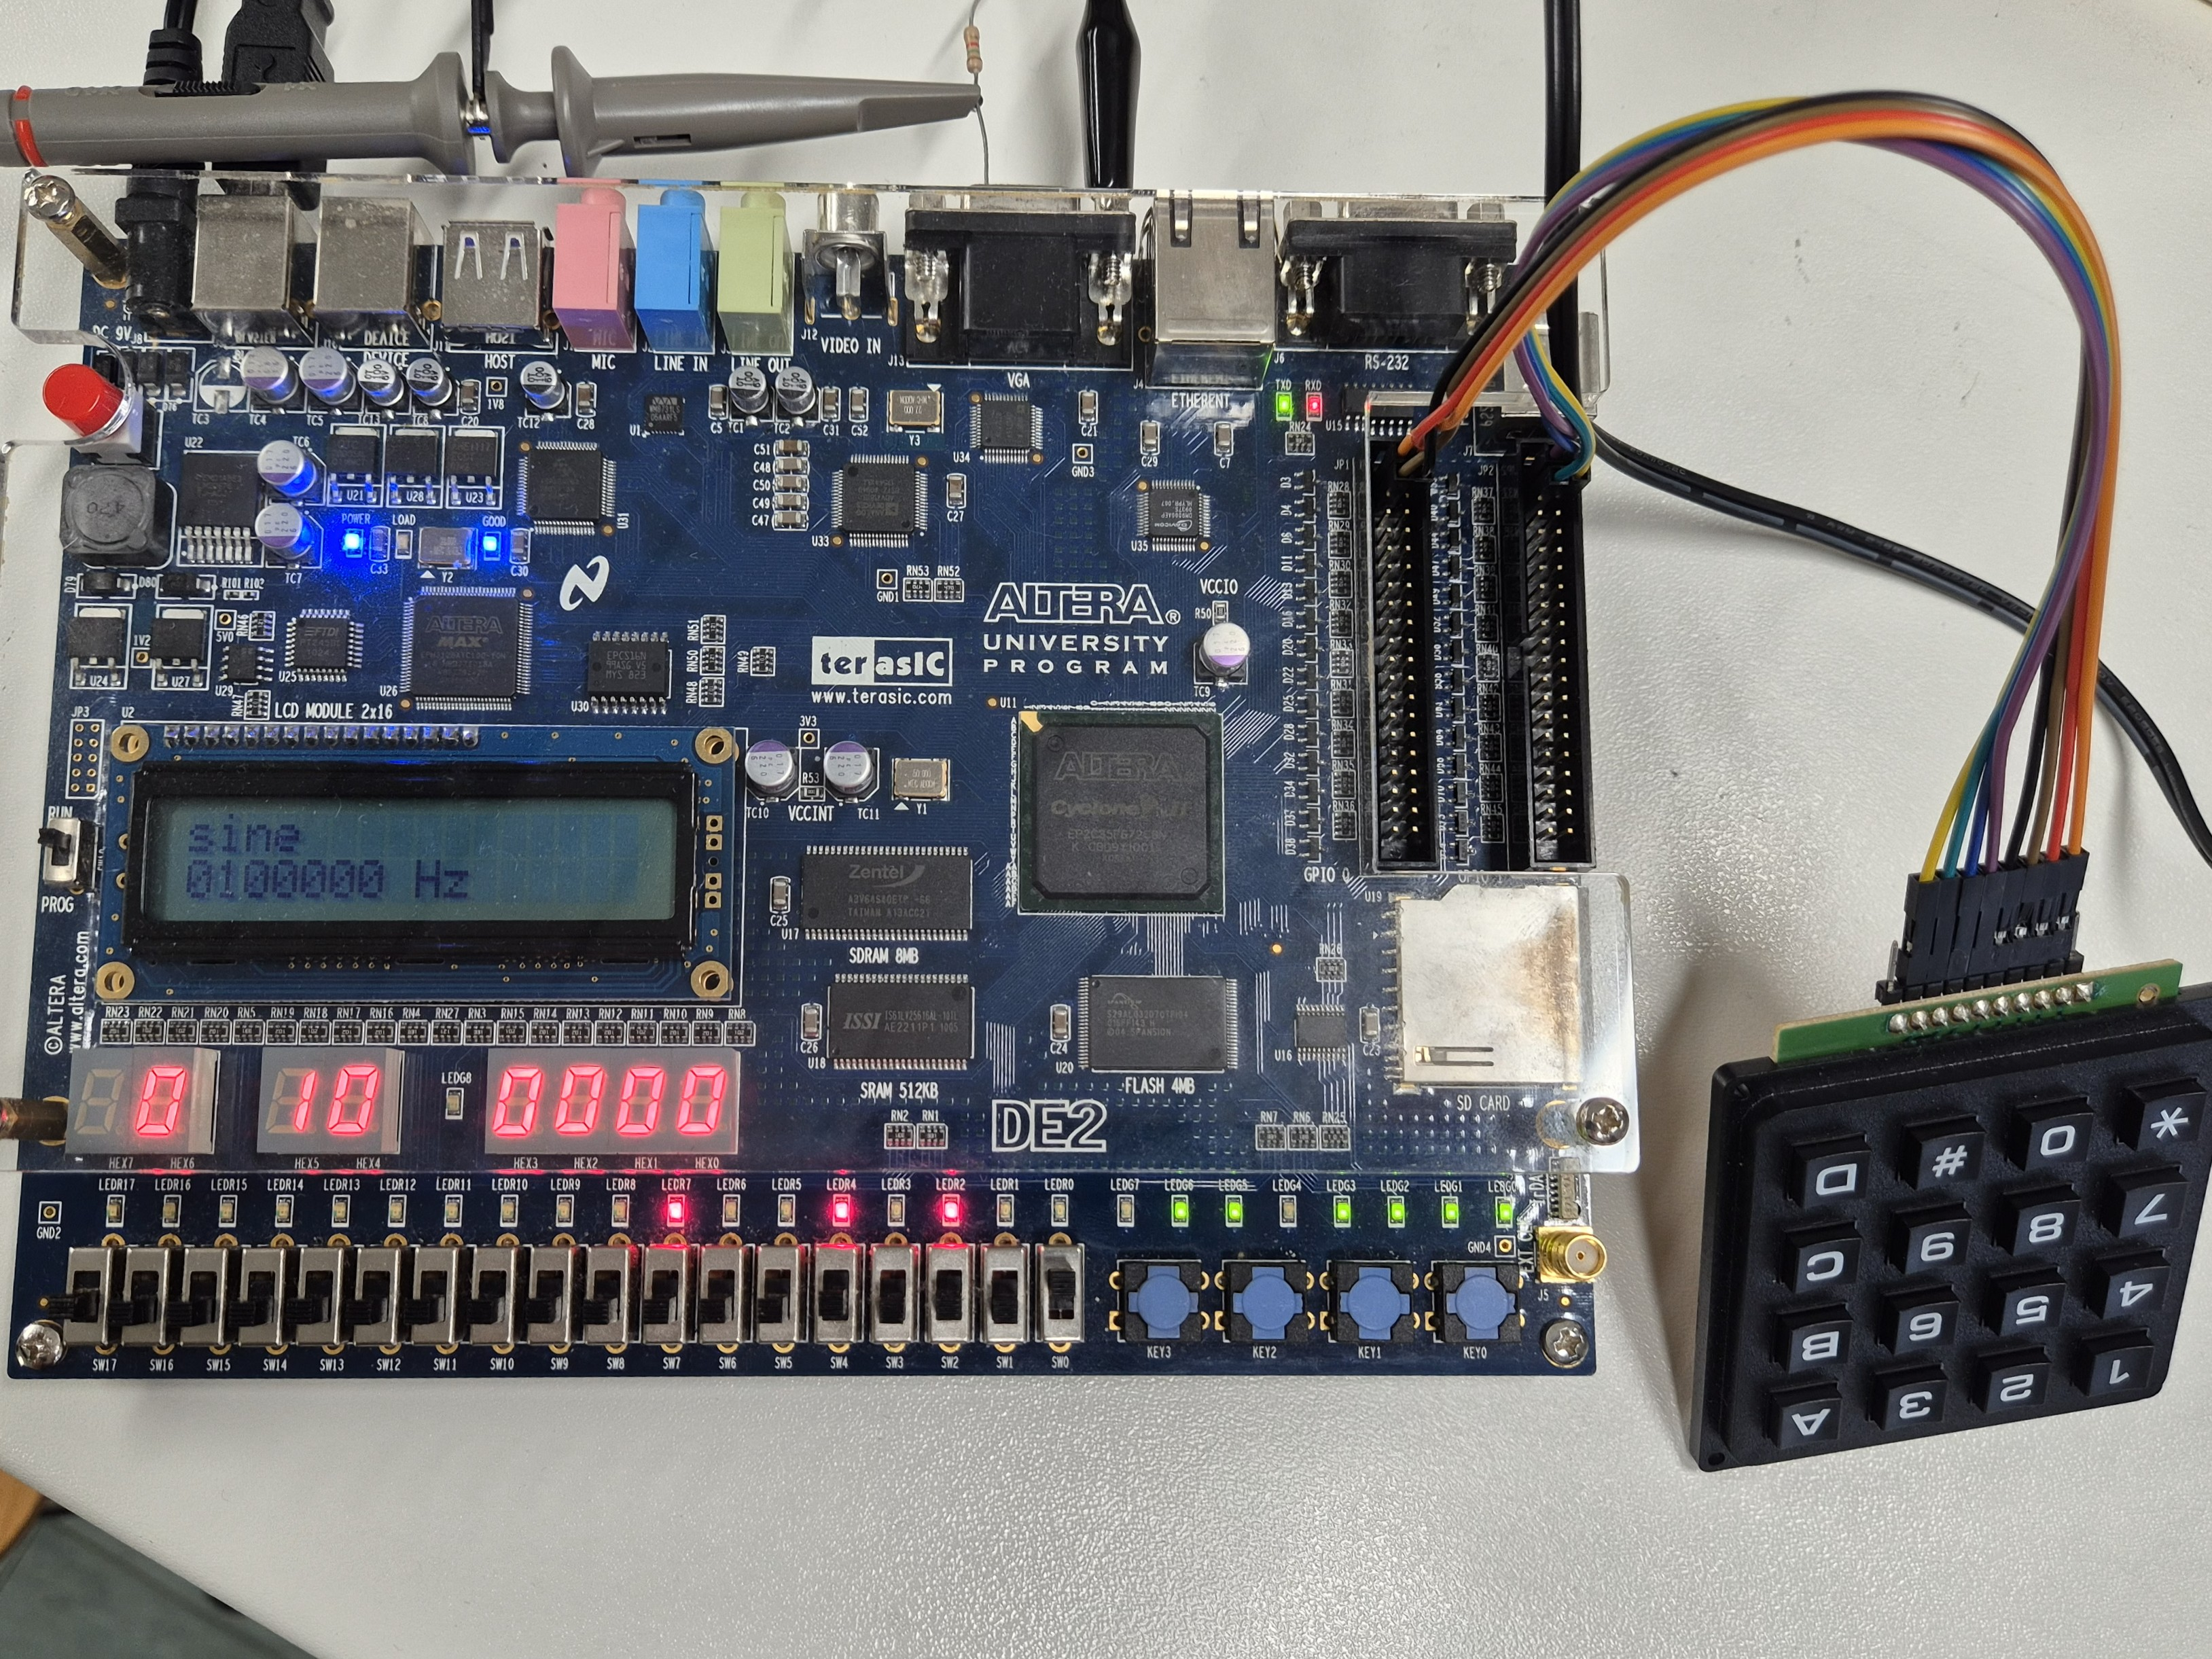
\includegraphics[width=0.8\textwidth]{img/final_test_img7.jpg}
    \caption{Selecting the sine wave with a 100kHz frequency}
    \label{fig:final_test_img7}
\end{figure}

\begin{figure}[h!]
    \centering
    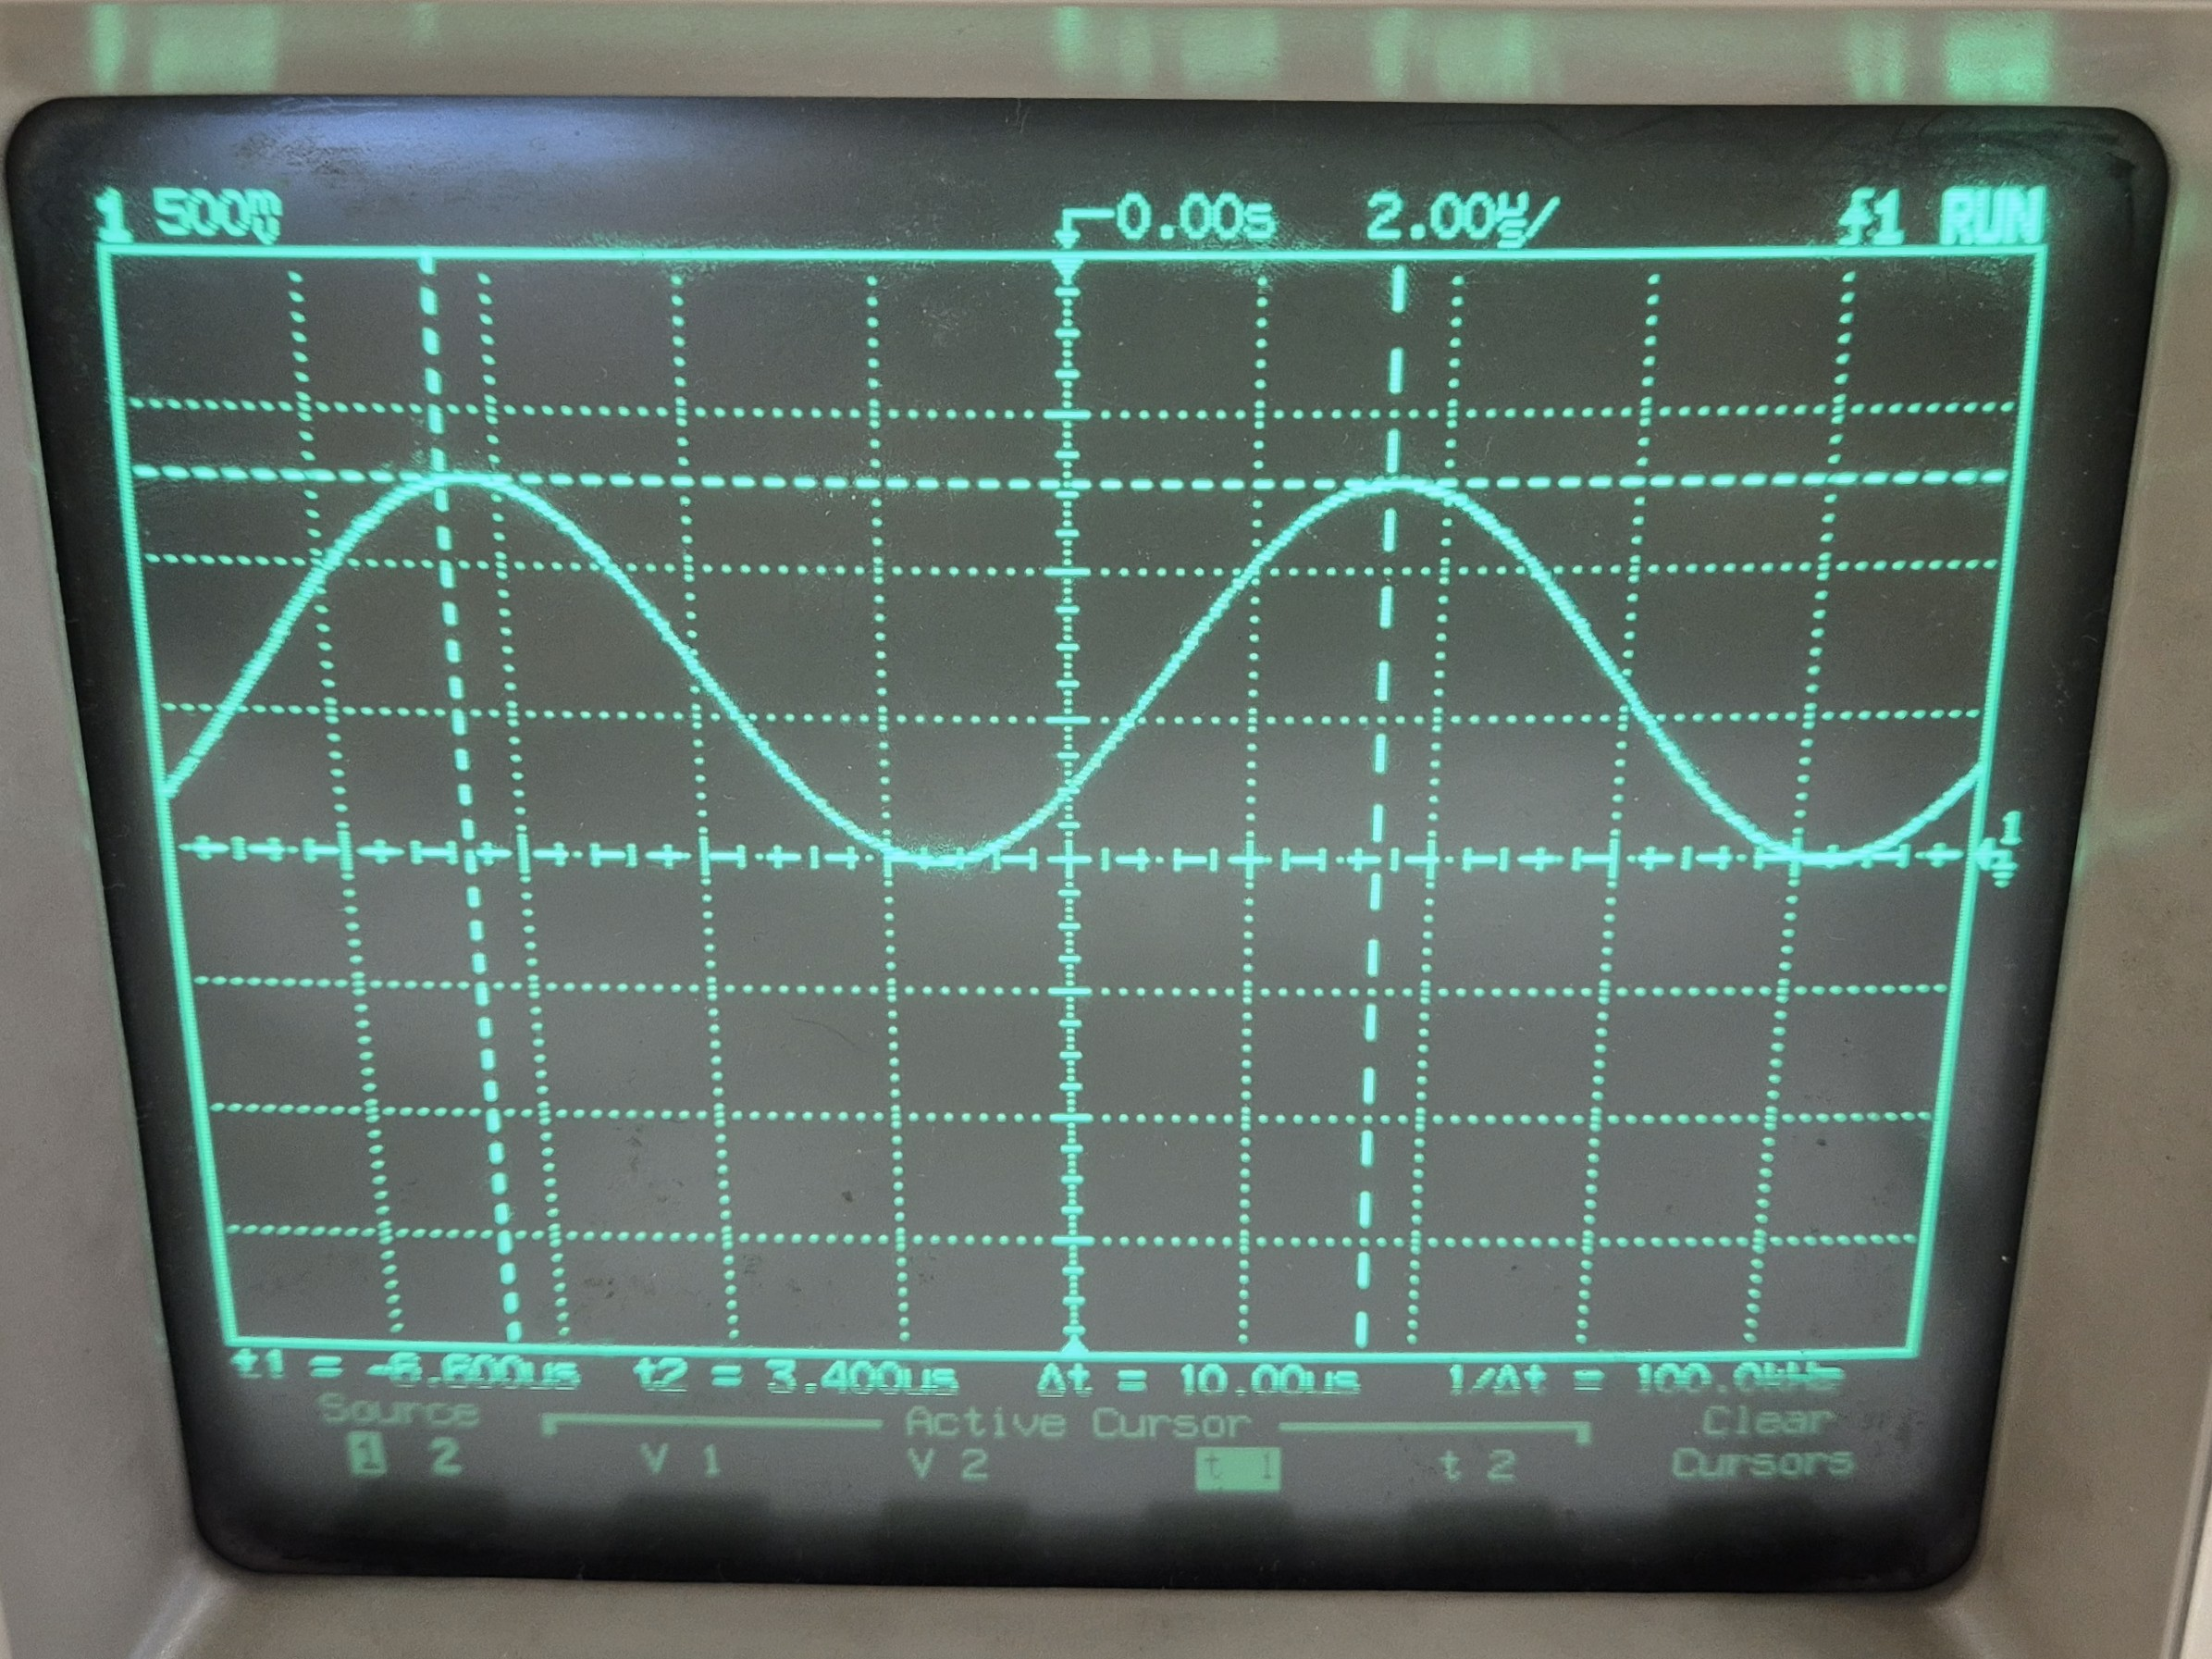
\includegraphics[width=0.8\textwidth]{img/final_test_img8.jpg}
    \caption{Sine wave, oscilloscope view}
    \label{fig:final_test_img8}
\end{figure}

\newpage

\begin{figure}[h!]
    \centering
    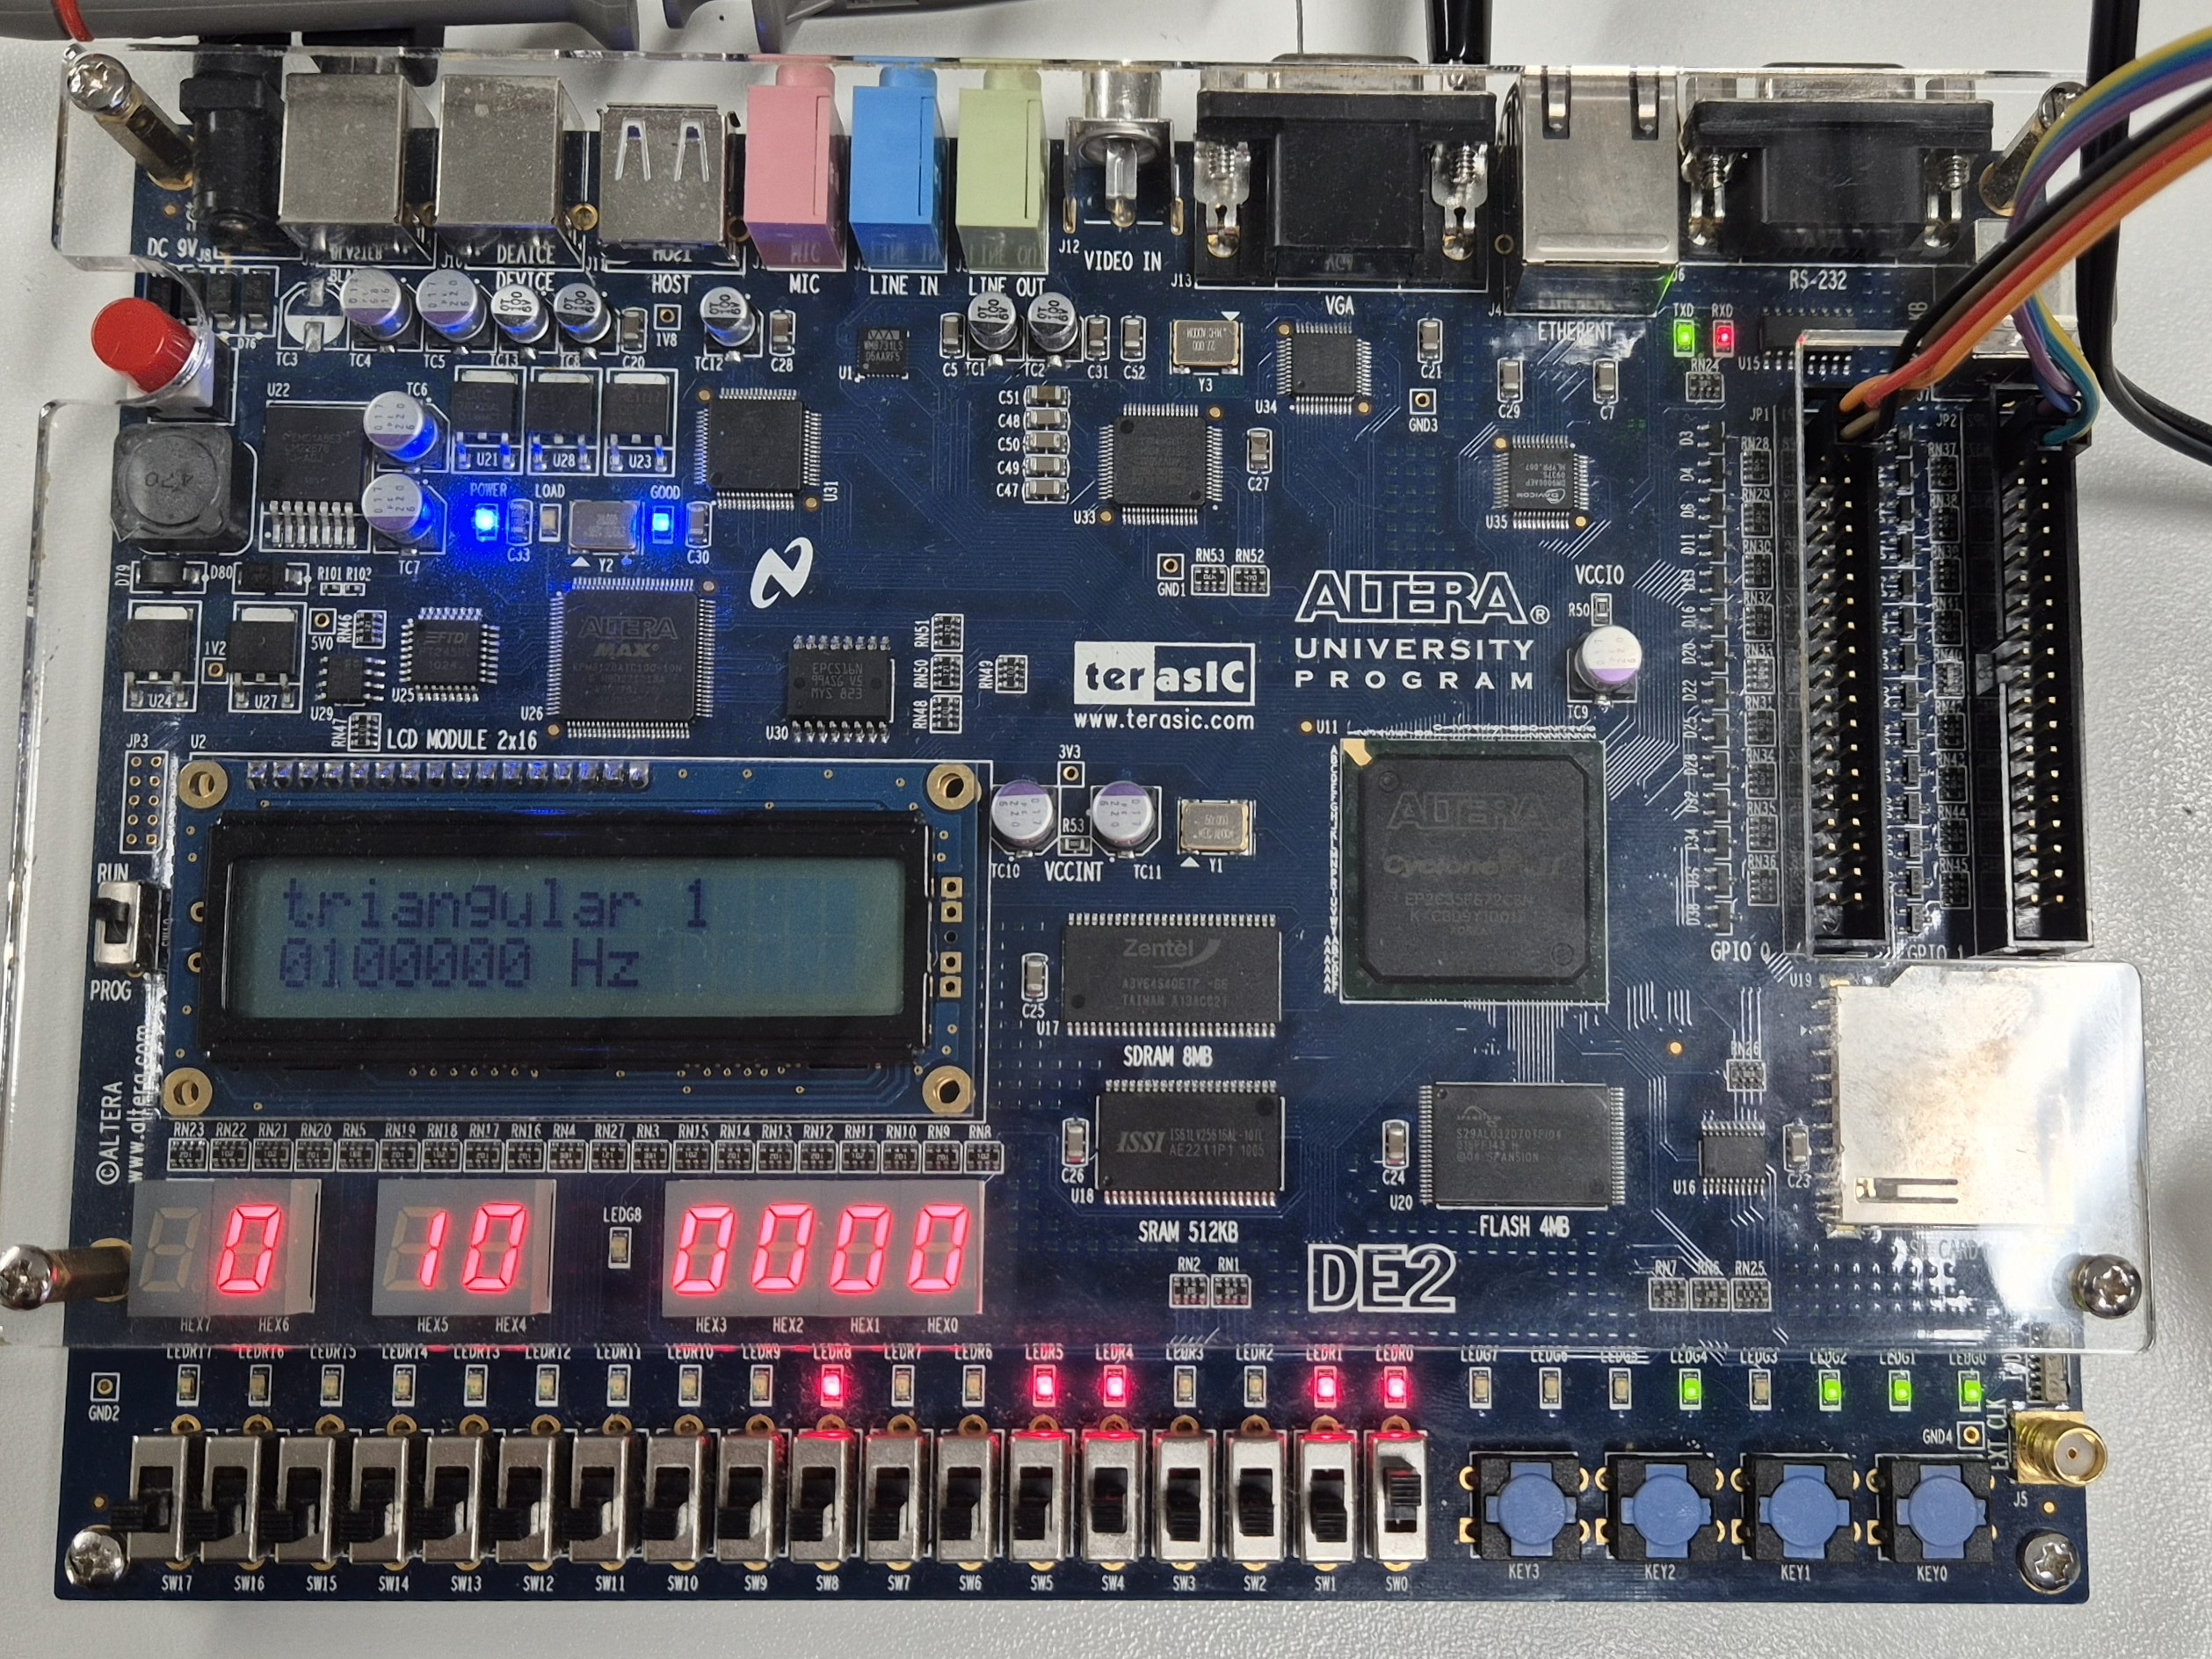
\includegraphics[width=0.8\textwidth]{img/final_test_img3.jpg}
    \caption{Selecting the sawtooth wave with a 100kHz frequency}
    \label{fig:final_test_img3}
\end{figure}

\begin{figure}[h!]
    \centering
    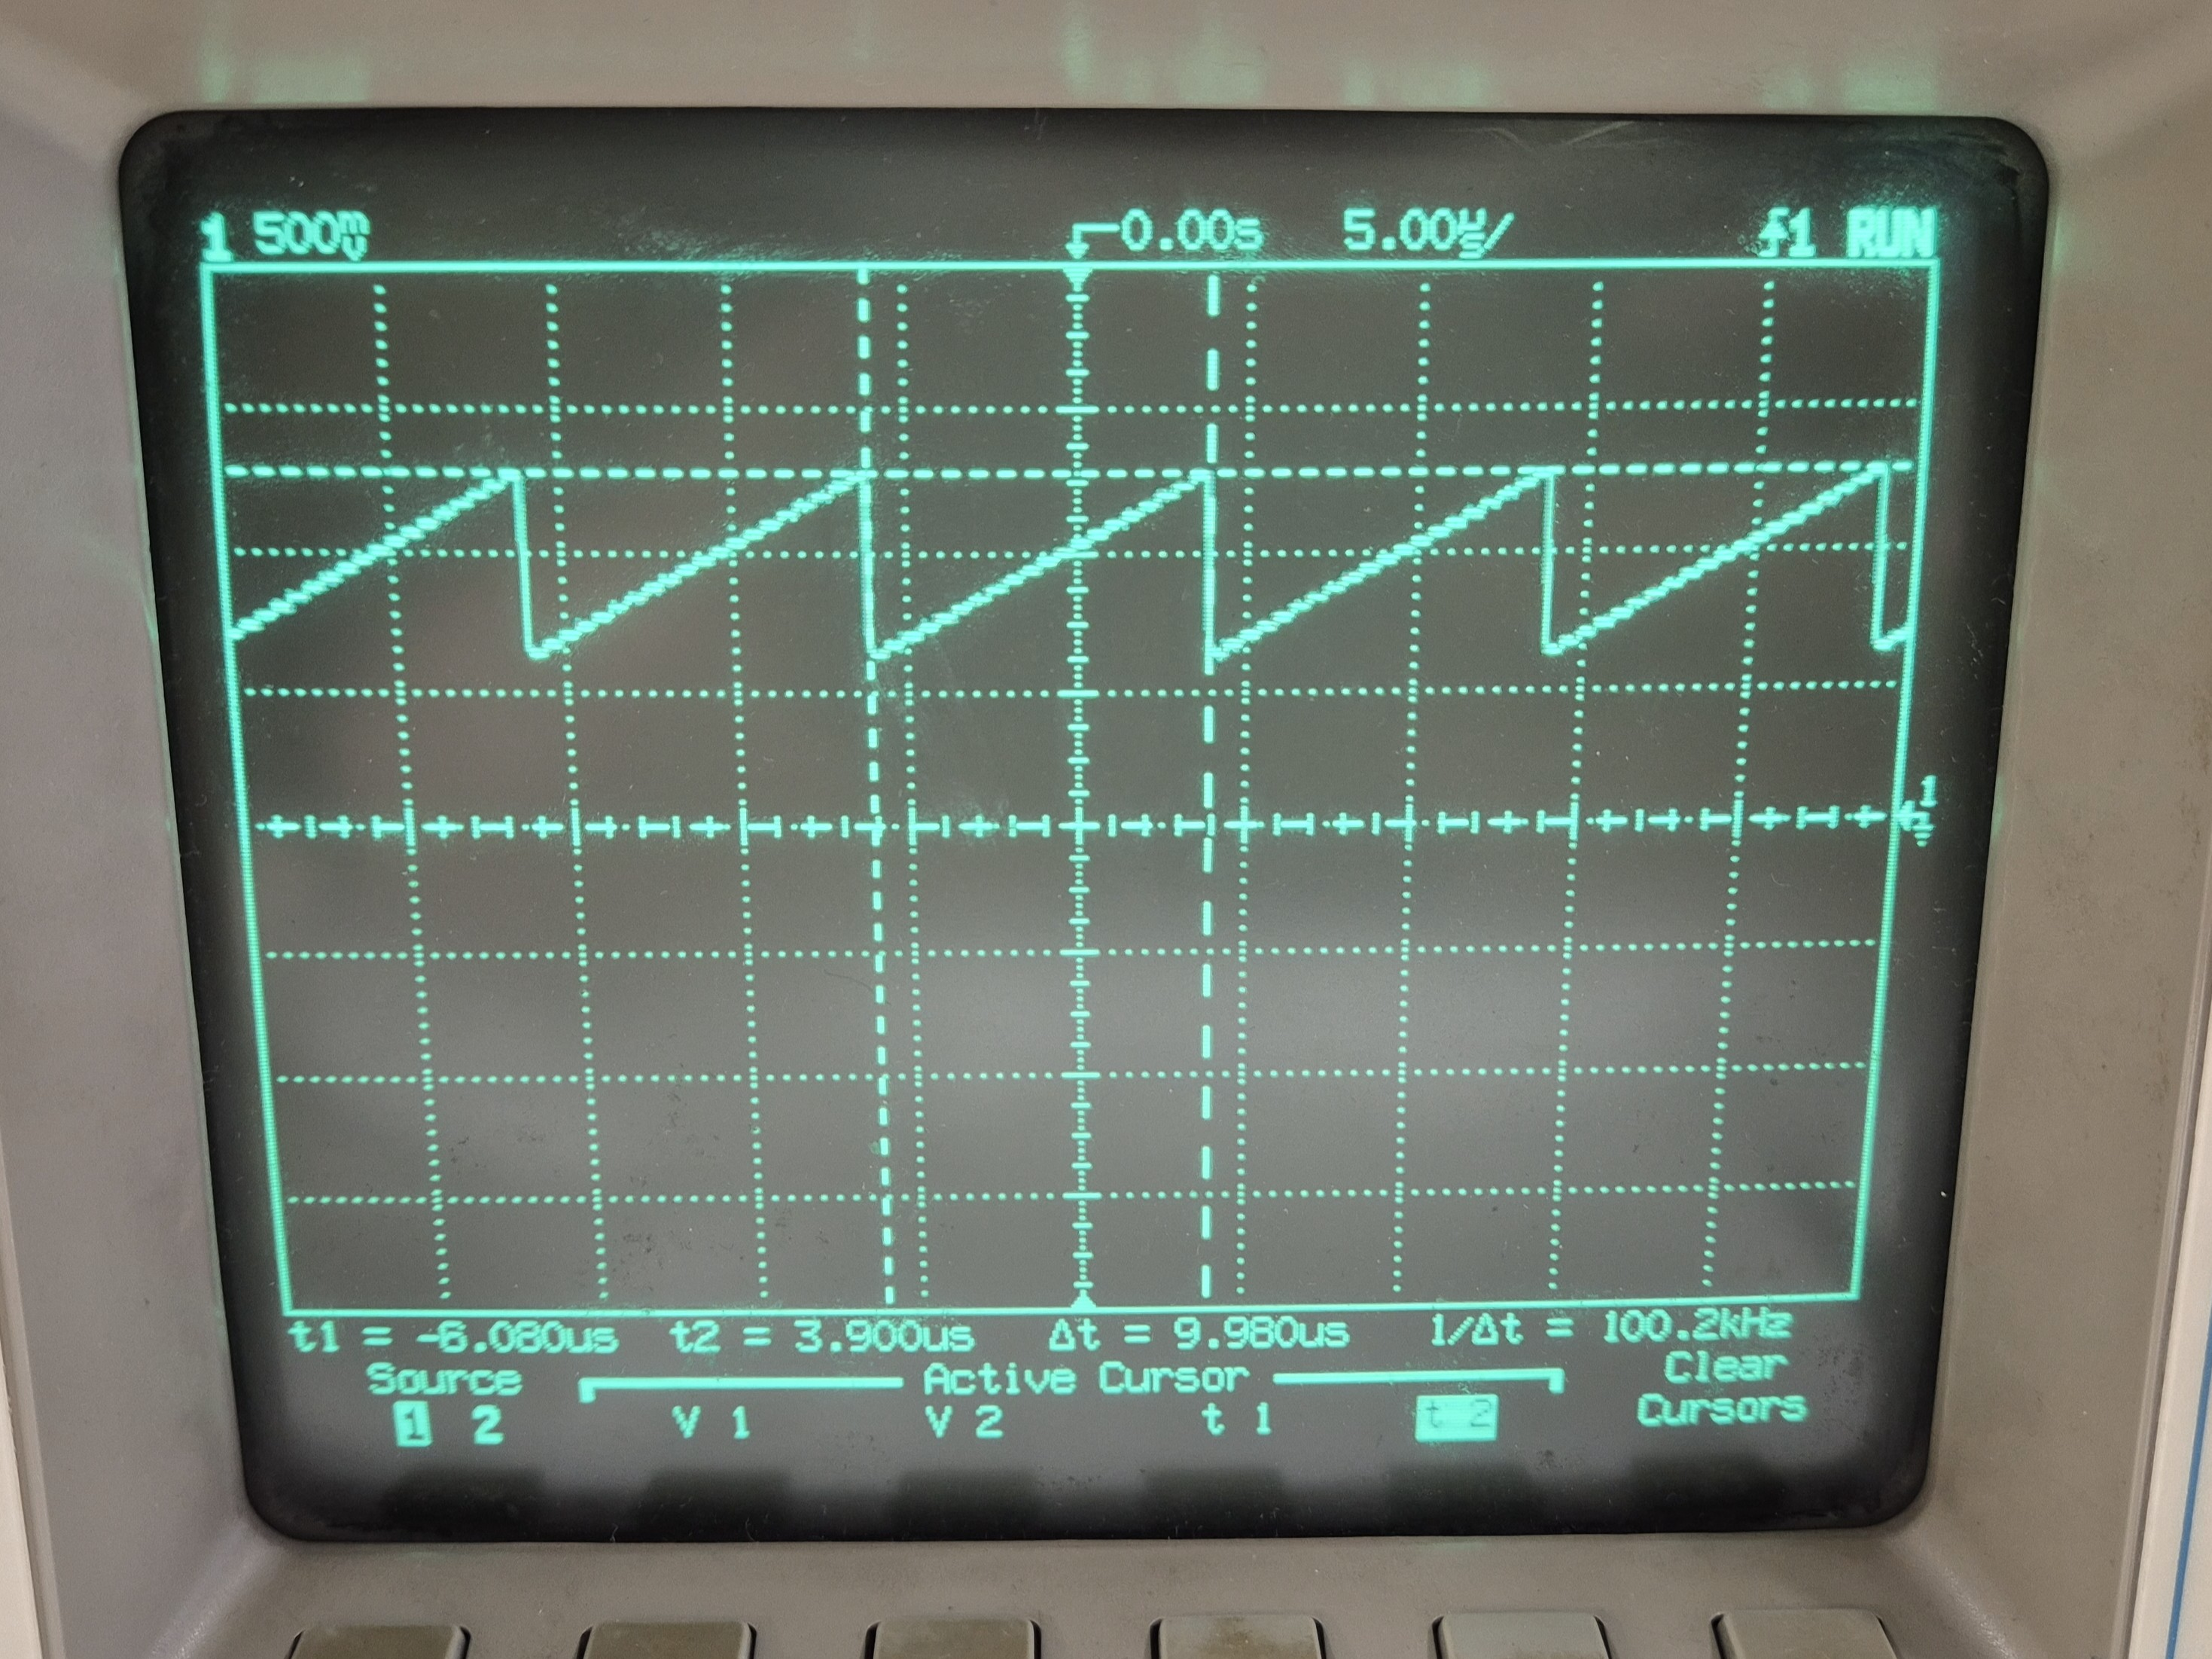
\includegraphics[width=0.8\textwidth]{img/final_test_img4.jpg}
    \caption{Sawtooth wave, oscilloscope view}
    \label{fig:final_test_img4}
\end{figure}

\newpage

\begin{figure}[h!]
    \centering
    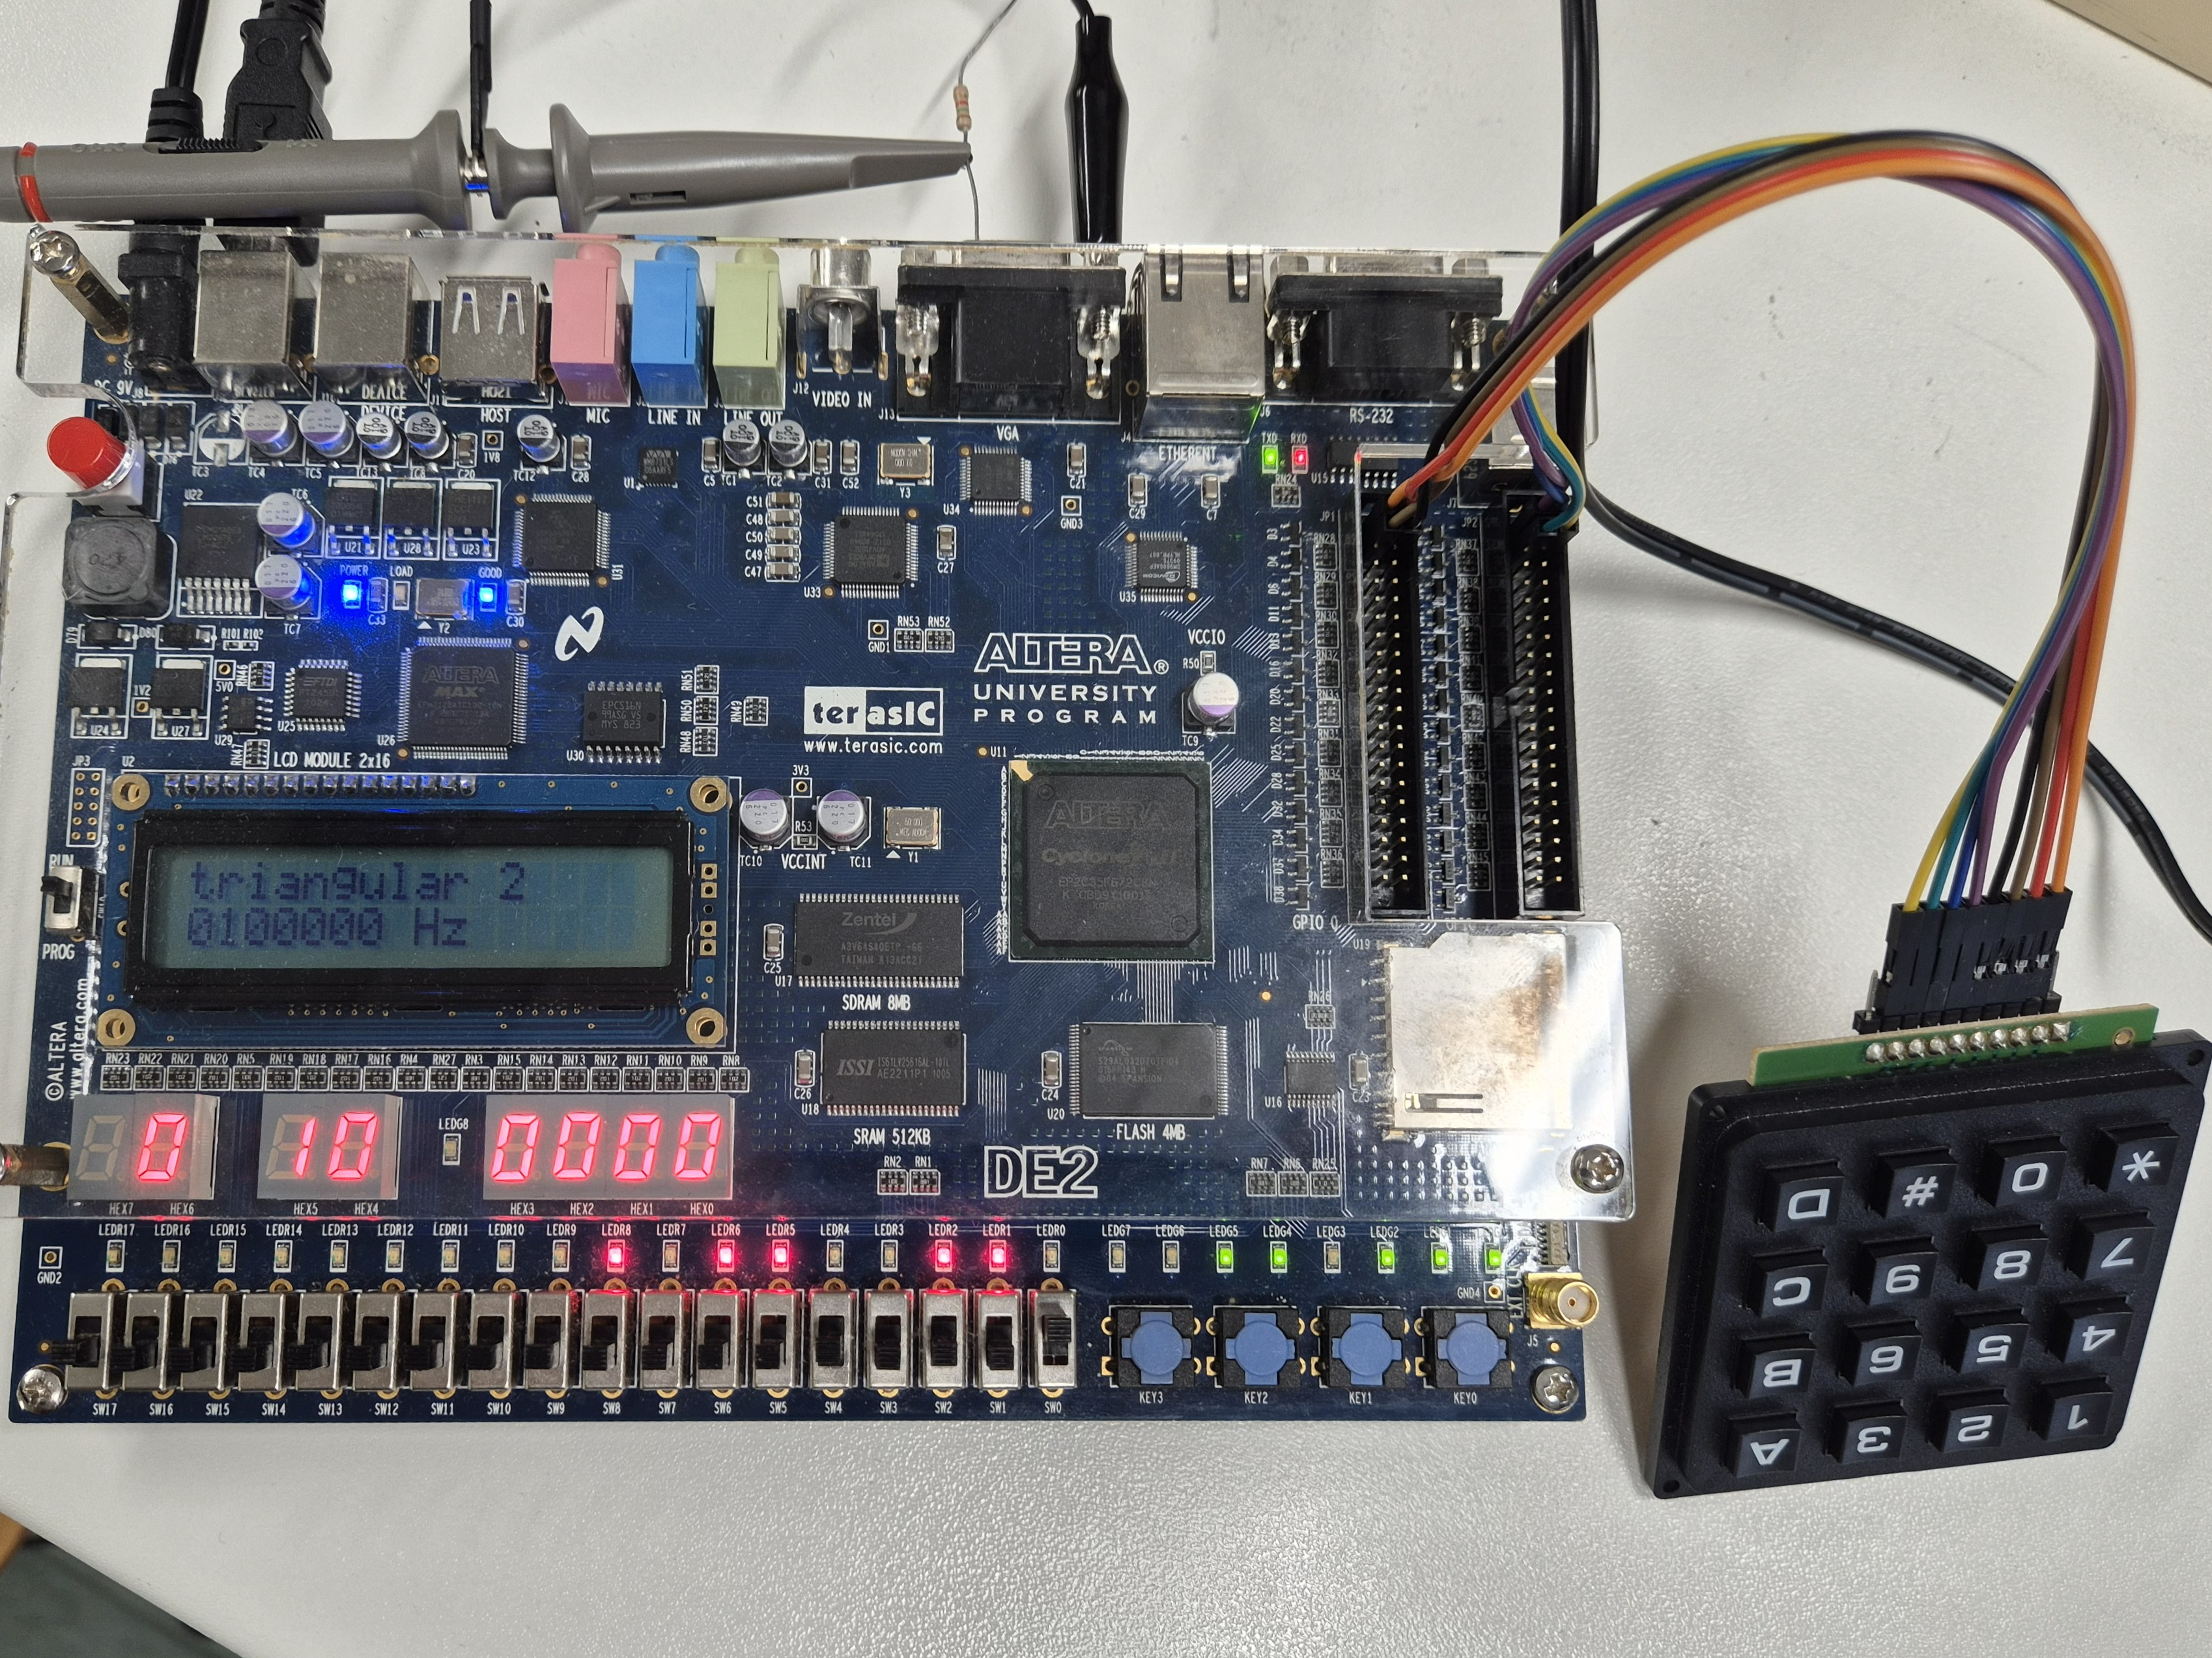
\includegraphics[width=0.8\textwidth]{img/final_test_img5.jpg}
    \caption{Quarter triangular x mirrored with a 100kHz frequency}
    \label{fig:final_test_img5}
\end{figure}

\begin{figure}[h!]
    \centering
    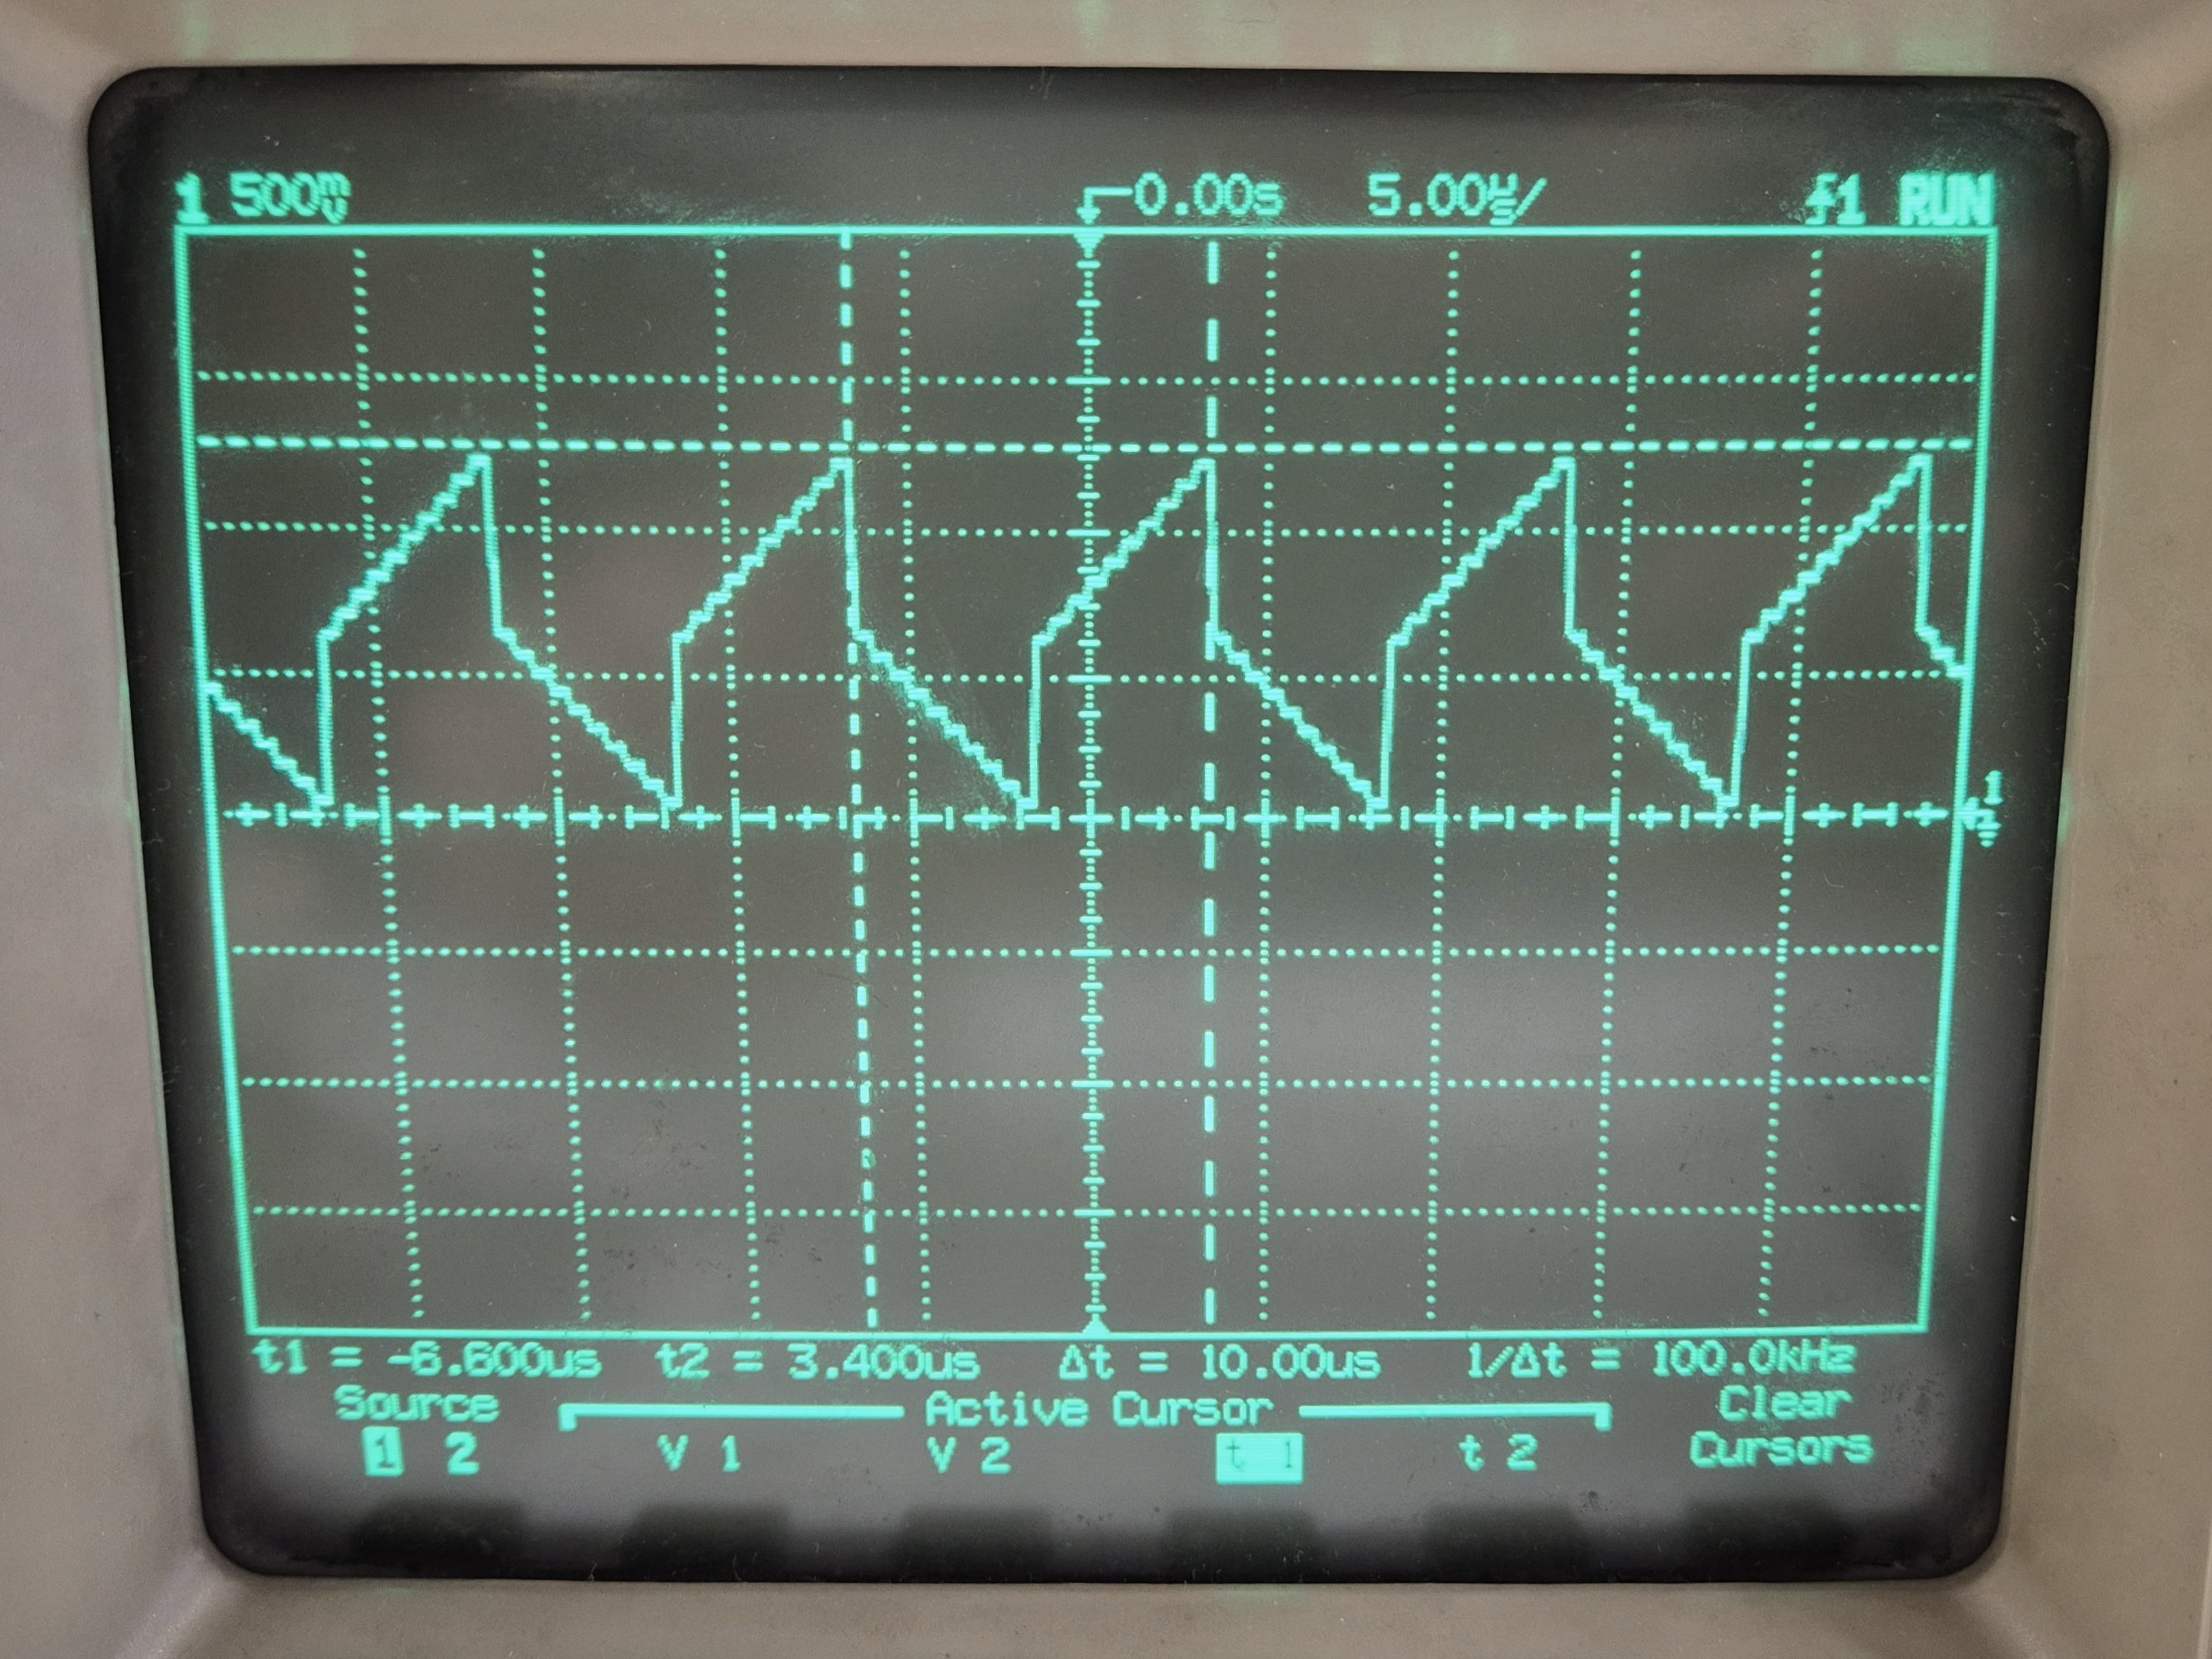
\includegraphics[width=0.8\textwidth]{img/final_test_img6.jpg}
    \caption{Quarter triangular x mirrored, oscilloscope view}
    \label{fig:final_test_img6}
\end{figure}

\newpage
\noindent
Another test that was conducted verified that the signal from the keypad module becomes increasingly difficult to read as the scan rate increases, until it becomes impossible to read at a clock rate of \(50 MHz\).

\vspace{0.5cm}
\begin{figure}[h!]
    \centering
    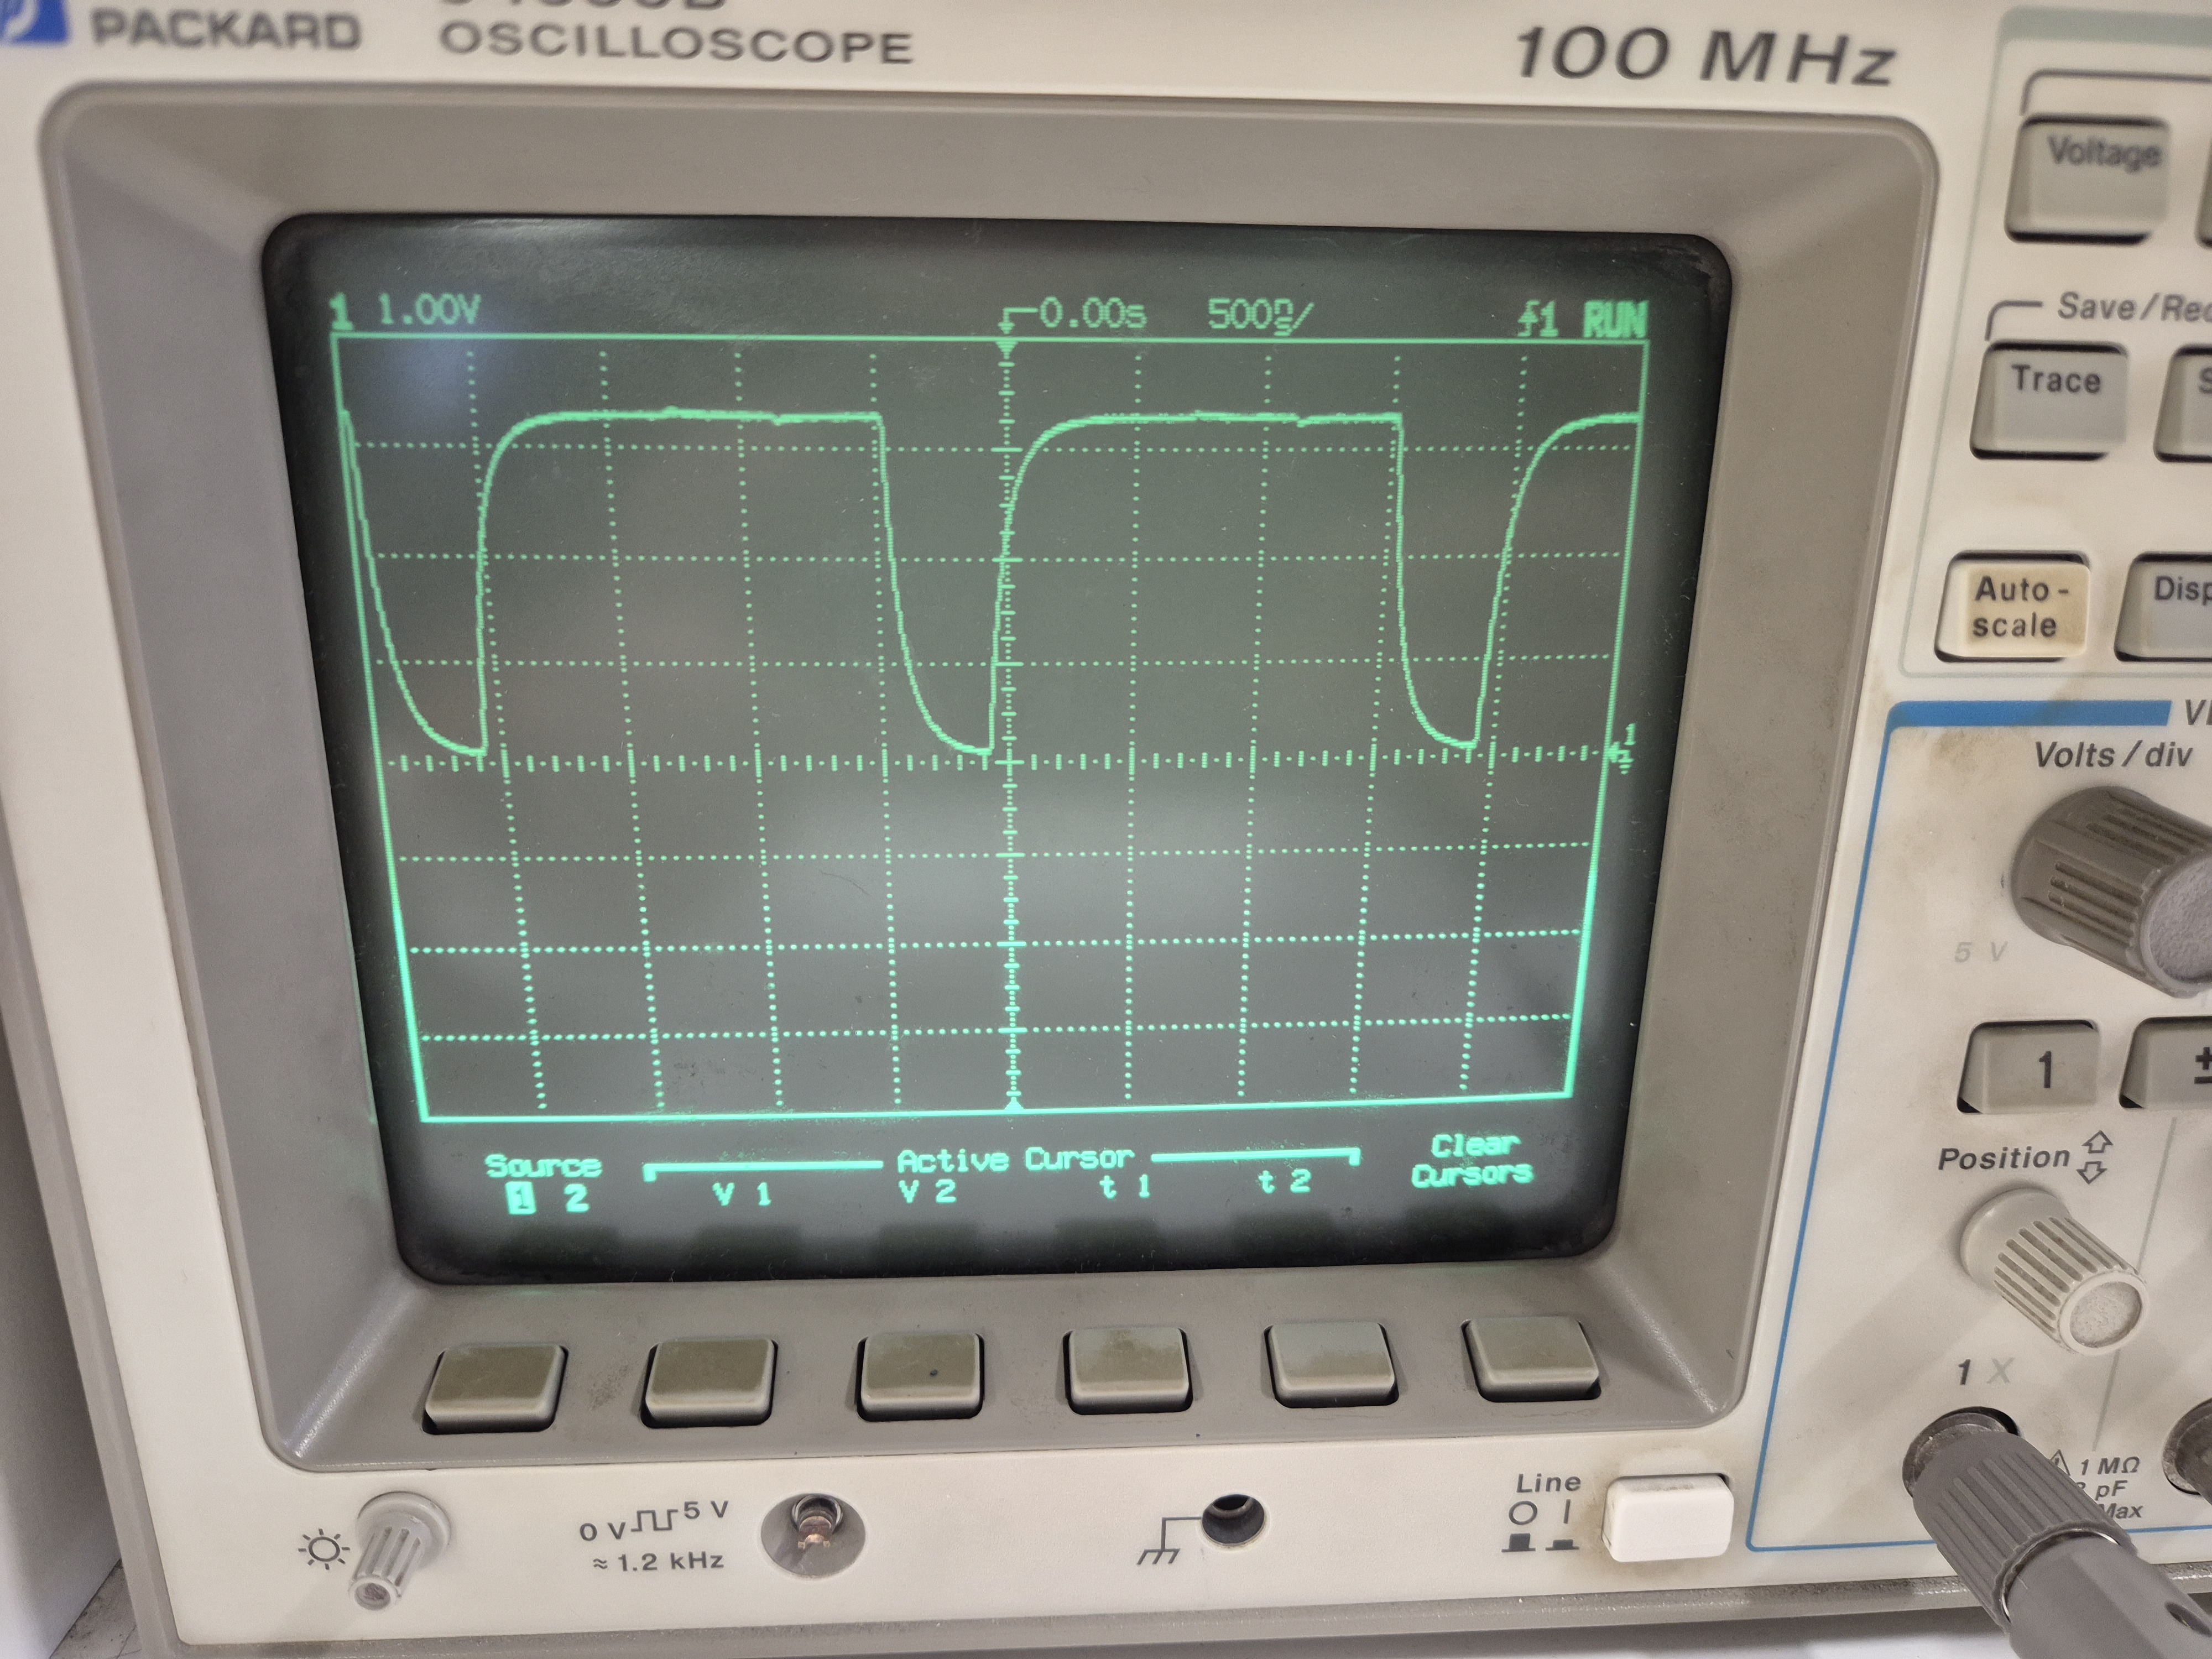
\includegraphics[width=0.8\textwidth]{img/5MHz_keypad.jpg}
    \caption{Signal read from the keypad with a scan frequency of 5MHz}
    \label{fig:5MHz_keypad}
\end{figure}

\begin{figure}[h!]
    \centering
    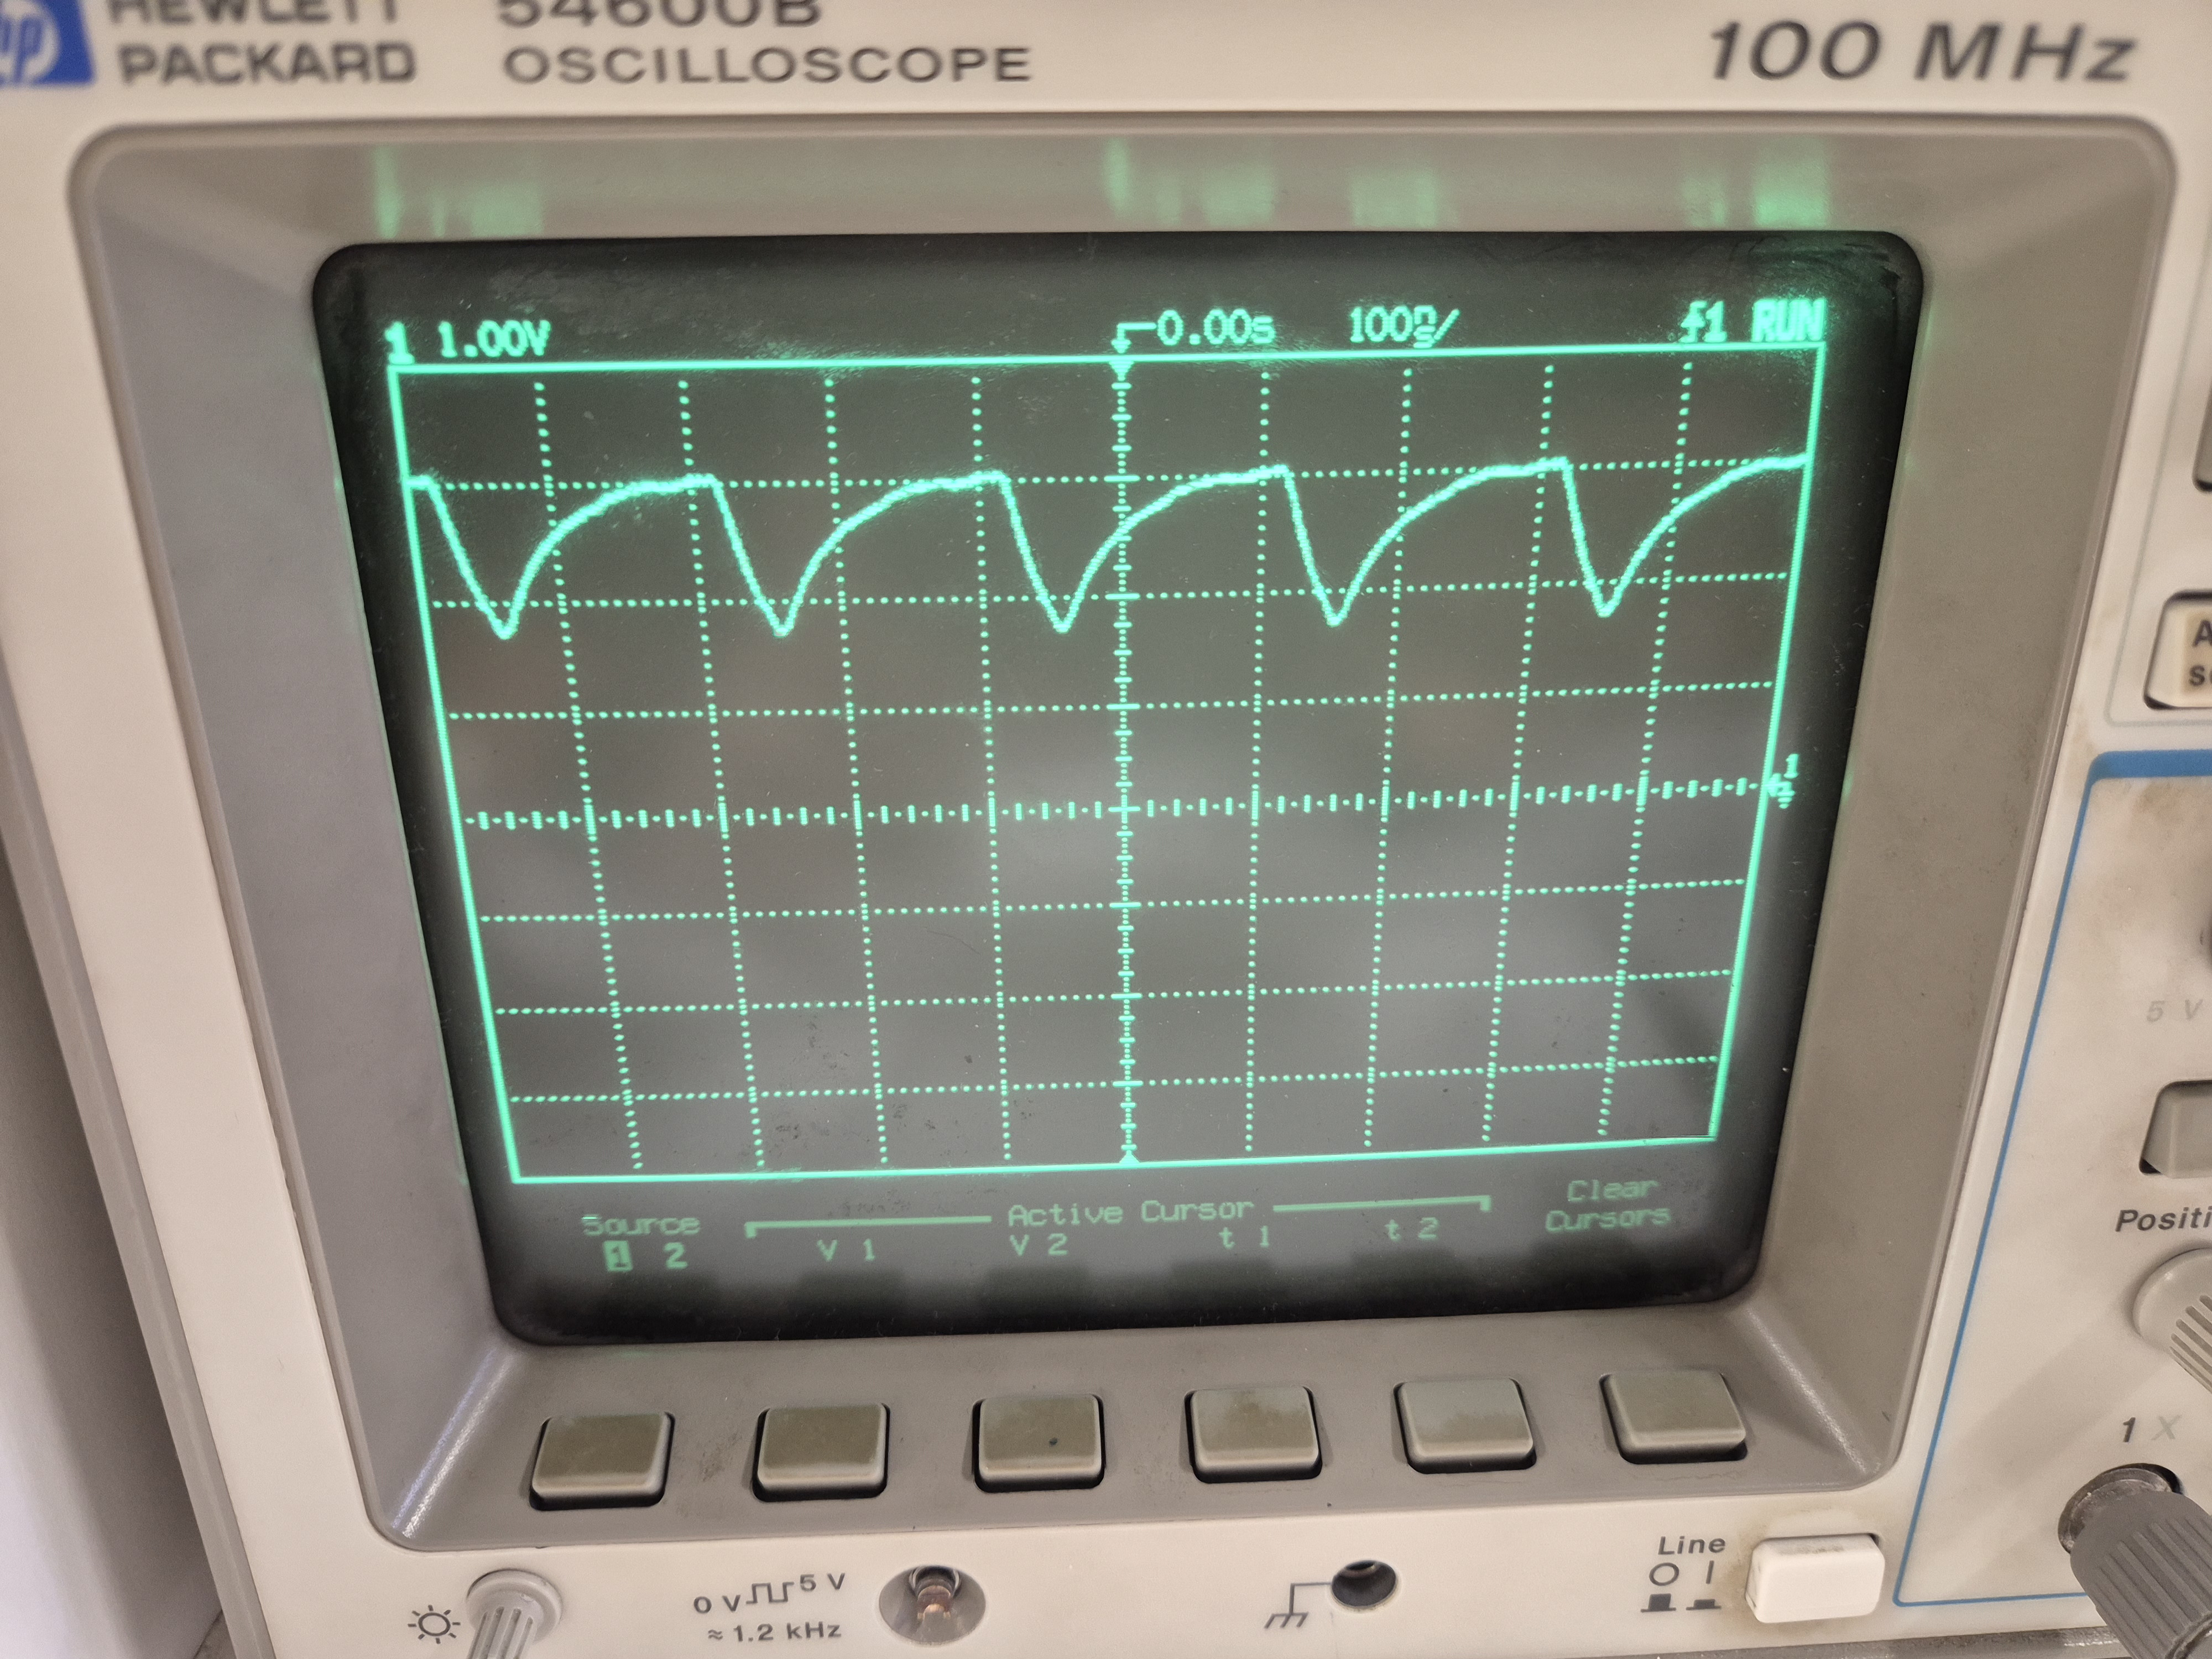
\includegraphics[width=0.8\textwidth]{img/50MHz_keypad.jpg}
    \caption{Signal read from the keypad with a scan frequency of 50MHz}
    \label{fig:50MHz_keypad}
\end{figure}

    
    \newpage
    \clearpage
\section{Implementation on Quartus}
\label{sec:implementation_on_quartus}

\subsection{Warnings}
The synthesis of the project on the Altera DE2 development board generates some warnings that are safe for the project, but it is important to analyze them to ensure the correct operation of the device. \\
The analysis of the warnings is separated for each module and for the main project that connects them together.

\subsubsection{LCD module}
The LCD module generate a lot of waring due to truncation of signals. \\
The first truncation warnings are as follows.

\begin{warningbox}[Warning]
    \text{Warning (10230): Verilog HDL assignment warning at lcd\_driver.v(*):} \newline
    \text{truncated value with size 64 to match size of target (32)}
\end{warningbox}

\noindent
They are generated for the \texttt{localparam} inside the \texttt{lcd\_driver} module, which contains the values of clock cycles to wait for a specific temporal delay.

\begin{lstlisting}[language=Verilog]
    localparam [31:0] wait40us = (CLK_FREQ/1000000)*40; 
    localparam [31:0] wait1ms = (CLK_FREQ/1000)*1; 
    localparam [31:0] wait2ms = (CLK_FREQ/1000)*2; 
    localparam [31:0] wait10ms = (CLK_FREQ/1000)*10; 
    localparam [31:0] wait20ms = (CLK_FREQ/1000)*20; 
    localparam [31:0] wait100ms = (CLK_FREQ/1000)*100; 
    localparam [31:0] wait2s = CLK_FREQ*2; 
\end{lstlisting}

\noindent
The operation on the right is performed automatically at \(64 bits\). \\
The other truncation warnings refer to the initialization file for the LUT.

\begin{warningbox}[Warning]
    \text{Warning (10230): Verilog HDL assignment warning at text\_lut\_init.txt(*):} \newline \text{truncated value with size 12 to match size of target (9)}
\end{warningbox}

\noindent
The instantiated \texttt{rom} has \(9 bit\) elements but is initialized with a hexadecimal file; for this reason, the first three bits are truncated, and the memory initialization file generated contains \(9 bit\) binary elements. \\
To allow, in the future, to add other page on the LCD, some memory location of the \texttt{rom} are left uninitialized, and this generate another warning.

\begin{warningbox}[Warning]
    \text{Warning (10850): Verilog HDL warning at text\_lut.v(16):} \newline
    \text{number of words (437) in memory file does not match the number of elements in the} \newline
    \text{address range [0:2047]}
\end{warningbox}

\newpage
\noindent
The instantiated \texttt{rom} memory is a read-only memory, so all the pins needed to write the memory are fixed at zero, generating the following warnings.

\begin{warningbox}[Warning]
    \text{Warning (10030): Net "rom.data\_a" at text\_lut.v(12) has no driver or initial value, using a} \newline
    \text{default initial value '0'} \newline
    \text{Warning (10030): Net "rom.waddr\_a" at text\_lut.v(12) has no driver or initial value, using a} \newline
    \text{default initial value '0'} \newline
    \text{Warning (10030): Net "rom.we\_a" at text\_lut.v(12) has no driver or initial value, using a} \newline
    \text{default initial value '0'}
\end{warningbox}

\subsubsection{DDFS module}
The DDFS module generates only truncation warnings due to the operations that are performed by default with signed integers at \(64 bits\).

\begin{warningbox}[Warning]
    \text{Warning (10230): Verilog HDL assignment warning at ddfs.v(*):} \newline
    \text{truncated value with size 64 to match size of target (12)} \newline
    \text{Warning (10230): Verilog HDL assignment warning at ddfs.v(*):} \newline
    \text{truncated value with size 64 to match size of target (10)}
\end{warningbox}

\noindent
The last warnings of this module are referred to the \texttt{rom} instance and are the same of the LCD module.

\begin{warningbox}[Warning]
    \text{Warning (10030): Net "rom.data\_a" at sin\_lut.v(17) has no driver or initial value, using a} \newline
    \text{default initial value '0'} \newline
    \text{Warning (10030): Net "rom.waddr\_a" at sin\_lut.v(17) has no driver or initial value, using a} \newline
    \text{default initial value '0'} \newline
    \text{Warning (10030): Net "rom.we\_a" at sin\_lut.v(17) has no driver or initial value, using a} \newline
    \text{default initial value '0'}
\end{warningbox}

\subsubsection{Keypad frequency module}
This module produce only truncation warnings due to the operations that are performed by default with signed integers at \(64 bits\).

\begin{warningbox}[Warning]
    \text{Warning (10230): Verilog HDL assignment warning at keypad\_freq\_sel\_module.v(49):} \newline
    \text{truncated value with size 64 to match size of target (32)}
\end{warningbox}

\noindent
Other truncation warnings are generated from the DDFS frequency converter module

\begin{warningbox}[Warning]
    \text{Warning (10230): Verilog HDL assignment warning at DDFS\_frequency\_converter.v(*):} \newline
    \text{truncated value with size 65 to match size of target (7)}
\end{warningbox}

\newpage
\noindent
This warning come from the following part of code

\begin{lstlisting}[language=Verilog]
    fw_1000000 <= (mult_1000000*K)>>54;
    fw_100000 <= (mult_100000*K)>>54;
    fw_10000 <= (mult_10000*K)>>54;
    fw_1000 <= (mult_1000*K)>>54;
    fw_100 <= (mult_100*K)>>54;
    fw_10 <= (mult_10*K)>>54;
    fw_2 <= (mult_2*K)>>54;
\end{lstlisting}

\noindent
where \texttt{mult\_*} contains the value of the frequency multiplied by powers of \(10\). \\
The value is shifted \(54\) times to the right, which is equivalent to dividing the value by \(2^{54}\).\\
This value can be stored in \(7 bits\), but the multiplied frequency needs \(65 bits\) to be represented, for this reason Quartus report a warning.


\subsubsection{Other warnings}
The other warning are related to the connection of the GPIOs and the instance or the optimization of the logic block inside the FPGA. \\
The optimization warning are as follows

\begin{warningbox}[Warning]
    \text{Warning (14284): Synthesized away the following node(s):} \newline
    \text{\quad $\Rdsh$ Warning (14285): Synthesized away the following RAM node(s):
} \newline
    \text{\quad \quad $\Rdsh$ Warning (14320): Synthesized away node "ddfs:inst\_ddfs\_mod ... ram\_block1a0"
}
\end{warningbox}

\noindent
The meaning of the warning is that an auto generated block has been removed due to synthesis optimization. \\
The reported example refers to a RAM block instantiated inside the \texttt{ddfs} module, but there are other similar warnings referring to DSP multiplier blocks instantiated inside the \texttt{keypad\_freq\_sel\_module}. \\
The GPIOs warning instead are different, the first type of GPIO warning are like follows

\begin{warningbox}[Warning]
    \text{Warning (13024): Output pins are stuck at VCC or GND} \newline
    \text{\quad $\Rdsh$ Warning (13410): Pin "LCD\_RW" is stuck at GND} \newline
    \text{\quad $\Rdsh$ Warning (13410): Pin "LCD\_ON" is stuck at VCC} \newline
    \text{\quad $\Rdsh$ Warning (13410): Pin "LCD\_BLON" is stuck at VCC} \newline
    \text{\quad $\Rdsh$ Warning (13410): Pin "VGA\_BLANK" is stuck at VCC} \newline
    \text{\quad $\Rdsh$ Warning (13410): Pin "VGA\_SYNC" is stuck at VCC} \newline
    \text{\quad $\Rdsh$ Warning (13410): Pin "HEX7[*]" is stuck at VCC}
\end{warningbox}

\noindent
This warning is normal for this design because some output pins of the FPGA are connected to the \texttt{blank} and \texttt{synch} pins of the VGA DAC, which are not used and are always disabled. \\
Other disabled pins are the \texttt{blon}, \texttt{rw}, and \texttt{on} pins of the LCD, used to set it in write mode and to keep the backlight always on. \\
The last disabled output pins are the seven-segment pins of the last seven-segment display, which are turned off because the display is not used. \\
There are two other types of GPIOs warning, because for the design has been used a \texttt{.qsf} file to automatically configure the output pins, but some of the pin are not used in the project, for this reason Quartus report them

\begin{warningbox}[Warning]
    \text{Warning (15705): Ignored locations or region assignments to the following nodes} \newline
    \text{\quad $\Rdsh$ Warning (15706): Node " ... " is assigned to location or region, but does not exist in design}
\end{warningbox}

\newpage
\noindent
furthermore some of the output pins have no defined the output capacitance value, so the software assign the default value of \(0 pF\) to all of them

\begin{warningbox}[Warning]
    \text{Warning (306006): Found 103 output pins without output pin load capacitance assignment}
\end{warningbox}

\newpage

\subsection{Timing analyzer}
To setup the timing analyzer is important to write the \texttt{.sdc} file where are defined the clock settings and the timing constrain for the input and output pins.

\subsubsection{Timing configuration file}
The clock signals in this project are three:

\begin{itemize}
    \item \texttt{CLOCK\_50} \\
    is the \(50\ \text{MHz}\) clock from the oscillator on the DE2 board.

    \item \texttt{CLOCK\_PLL} \\
    is the clock output of the PLL. This clock source is generated from the \texttt{CLOCK\_50} clock by multiplying it by 7/5.\\
    This is a \(70\ \text{MHz}\) clock source with the same phase as \texttt{CLOCK\_50}.

    \item \texttt{CLK\_FREQ\_DIV} \\
    is the output of the frequency divider instantiated inside the \texttt{ddfs} module.\\
    The problem with this clock source is that the frequency can be selected through the external pins of the module; for the analysis, it has been configured at its maximum frequency, which is \texttt{CLOCK\_PLL} divided by two.

\end{itemize}

\noindent
the part of code used to set up the clock signals is the following

\vspace{0.5cm}
\begin{lstlisting}[language=sdc, caption=Clock settings for timing analyzer]
    create_clock 
        -name {CLOCK_50} 
        -period 20.000 
        -waveform {0.000 10.000} 
        { CLOCK_50 }
        
    create_generated_clock 
        -name {CLOCK_PLL} 
        -source {inst_pll|altpll_component|pll|inclk[0]}
        -divide_by 5 -multiply_by 7
        -duty_cycle 50.00 -phase 0.0 -offset 0.0 
        { inst_pll|altpll_component|pll|clk[0] }
        
    create_generated_clock 
        -name {CLK_FREQ_DIV} 
        -source {inst_pll|altpll_component|pll|clk[0]} 
        -divide_by 2 -multiply_by 1 
        -duty_cycle 50.00 
        { ddfs:inst_ddfs_mod|freq_divider_DDFS:f_div_inst|clk_out }
    
\end{lstlisting}
\vspace{0.5cm}

\newpage
\noindent
Now that we have defined the clock, we must add the input and output timing constrain. \\
First we define the asynchronous input and output pins, in our case the asynchronous pins are the
\begin{itemize}
    \item Switch input pins
    \item Seven segment display output pins
    \item led output pins
    \item \texttt{GPIO\_0} pins \\
    this pins are connected the row of the keypad module, the pression of a button of the keypad can be asynchronous and the input is protected with a latch chain.
\end{itemize}

the part of code used to setup the asynchronous path is the following

\vspace{0.5cm}
\begin{lstlisting}[language=sdc, caption=Setup asynchronous paths]
    set_false_path 
        -from [get_ports {GPIO_0[0] GPIO_0[1] GPIO_0[2] GPIO_0[3] SW[*]}]
    set_false_path 
        -to [get_ports {HEX0[*] HEX1[*] ... HEX5[*] HEX6[*] HEX7[*]}]
    set_false_path 
        -to [get_ports {LEDR[*] LEDG[*]}]
    
\end{lstlisting}
\vspace{0.5cm}

\noindent
Now it is time to set the timing constraints for the synchronized outputs.\\
To do this, we use the \texttt{set\_input\_delay} and \texttt{set\_output\_delay} commands.\\
These commands take two parameters: \texttt{-clock}, which is the reference clock for the specified input or output, and \texttt{-min} or \texttt{-max}, which refer to hold and setup timing constraints, respectively, and are referenced to the clock edge, as shown in \autoref{fig:min_max_delay}.

\vspace{0.5cm}
\begin{figure}[h!]
    \centering
    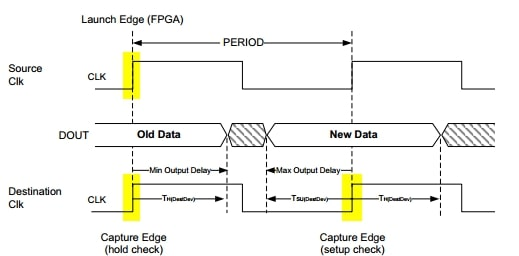
\includegraphics[width=0.6\textwidth]{img/min_max_delay.jpg}
    \caption{min and max delay timing interpretation}
    \label{fig:min_max_delay}
\end{figure}
\vspace{0.5cm}

\newpage
\noindent
For the GPIO outputs, which are connected to the keypad, and for the LCD outputs, the signals are synchronized with the \texttt{CLOCK\_PLL} source; however, the devices driven by these signals do not have a clock input. \\
For the LCD, the timing constraints are controlled by the \texttt{lcd\_driver}, and the keypad is a passive device, so it does not have digital circuits for synchronization. \\
For this reason, the constraints for these pins are arbitrary. \\
For the VGA output, we use the datasheet values for setup and hold times (respectively \(1.5ns\) and \(2.5ns\)) and choose slightly larger values to ensure safe operation.
The code to set up these timing constraints is the following

\vspace{0.5cm}
\begin{lstlisting}[language=sdc, caption=Setup synchronous paths]
    #the LCD and GPIO_1 outputs are not synchronized; 
    #therefore, the clock limits within a cycle are arbitrary
    set_output_delay 
        -min 1 [get_ports {GPIO_1[0] GPIO_1[1] GPIO_1[2] GPIO_1[3]}] 
        -clock [get_clocks CLOCK_PLL]
    set_output_delay 
        -max 1 [get_ports {GPIO_1[0] GPIO_1[1] GPIO_1[2] GPIO_1[3]}] 
        -clock [get_clocks CLOCK_PLL]
    set_output_delay 
        -min 1 [get_ports LCD*] 
        -clock [get_clocks CLOCK_PLL]
    set_output_delay 
        -max 1 [get_ports LCD*] 
        -clock [get_clocks CLOCK_PLL]
    
    #from datasheet min = thold = 2.5ns; max = tsetup = 1.5ns
    #we take some margin
    set_output_delay 
        -min 3 [get_ports VGA*] 
        -clock [get_clocks CLK_FREQ_DIV]
    set_output_delay 
        -max 2 [get_ports VGA*] 
        -clock [get_clocks CLK_FREQ_DIV]
    
\end{lstlisting}
\vspace{0.5cm}

\newpage
\subsubsection{Timing slack and critical path}
The timing analyzer uses the library of the FPGA macro-cells to verify that the timing constraints are respected for both the slow and fast models.\\
The slow model is used to check the maximum frequency of the clock sources (at a temperature of \(85^\circ C\)) and the setup timing constraints.\\
The fast model is used to verify that hold time violations do not occur (at a temperature of \(0^\circ C\)).

\paragraph{Slow model} \quad \\
As we can see in \autoref{fig:f_max}, the maximum calculated frequency for each clock source is higher than the frequency used.

\vspace{0.5cm}
\begin{figure}[h!]
    \centering
    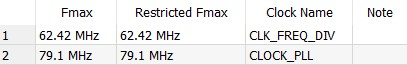
\includegraphics[width=0.6\textwidth]{img/Fmax.jpg}
    \caption{Maximum clock frequency for every clock source}
    \label{fig:f_max}
\end{figure}
\vspace{0.5cm}

\noindent
The maximum frequency is a consequence of setup time violations; in fact, from the setup time slack, we can calculate the maximum frequency for each clock source. \\
The maximum frequency is only computed for paths where the source and destination registers or ports are driven by the same clock.

\vspace{0.5cm}
\begin{figure}[h!]
    \centering
    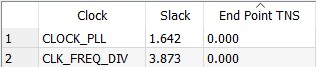
\includegraphics[width=0.45\textwidth]{img/Setup_slack.jpg}
    \caption{Setup time slack}
    \label{fig:setup_slack}
\end{figure}

\noindent
The slack reported in \autoref{fig:setup_slack} is related to the entire system, so the value represents the worst slack considering the interaction of the two clock sources. \\
The two paths that reduce the slack of the clock sources are shown in \autoref{fig:CLK_FREQ_DIV_slack} and in \autoref{fig:CLOCK_PLL_slack}

\vspace{0.5cm}
\begin{figure}[h!]
    \centering
    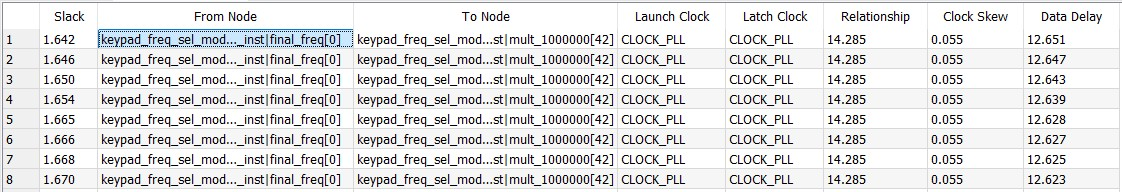
\includegraphics[width=1\textwidth]{img/CLOCK_PLL slack.jpg}
    \caption{CLOCK\_PLL setup time slack}
    \label{fig:CLOCK_PLL_slack}
\end{figure}

\begin{figure}[h!]
    \centering
    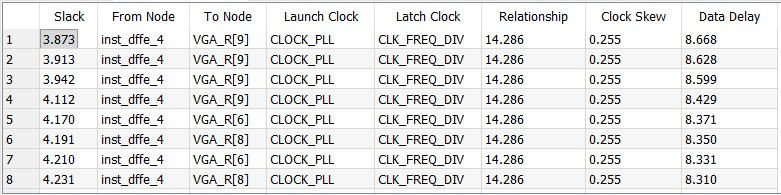
\includegraphics[width=0.8\textwidth]{img/CLK_FREQ_DIV slack.jpg}
    \caption{CLK\_FREQ\_DIV setup time slack}
    \label{fig:CLK_FREQ_DIV_slack}
\end{figure}

\newpage
\noindent
\paragraph{Critical path} \quad \\
From the analysis done with the slow model for the setup time slack,we can see that for the \\
\texttt{CLOCK\_PLL} source, the critical path is referred to the shift and add operation done into the \\
\texttt{DDFS\_frequency\_converter} module

\begin{lstlisting}[language=Verilog]
    mult_1000000 <=
    (final_freq<<19)+(final_freq<<18)+(final_freq<<17)+(final_freq<<16)
    +(final_freq<<14)+(final_freq<<9)+(final_freq<<6)
\end{lstlisting}

\noindent
For the \texttt{CLK\_FREQ\_DIV} source, indeed the critical path came from the connection between the mirror input of the \text{DDFS} module and the DAC output. \\
The critical path is referred to this two combinational blocks inside the module

\begin{lstlisting}[language=Verilog]
    if(mirror_x && mirror_y) begin
        //third quarter or fourth quarter
            ...
            
    end else if(mirror_x) begin
        //second quarter or fourth quarter
            ...
            
    end
\end{lstlisting}

\begin{lstlisting}[language=Verilog]
    if(mirror_y)
        //second quarter or fouth quarter
            ...
\end{lstlisting}

\noindent
This blocks was previously analyzed in
\autoref{sec:description_of_the_architecture} (\autoref{lst:DDFS_output_calculation} and \autoref{lst:DDFS_address}). \\
In the Chip Planner, we can see where these two critical paths are located inside the FPGA.

\begin{figure}[h!]
    \centering
    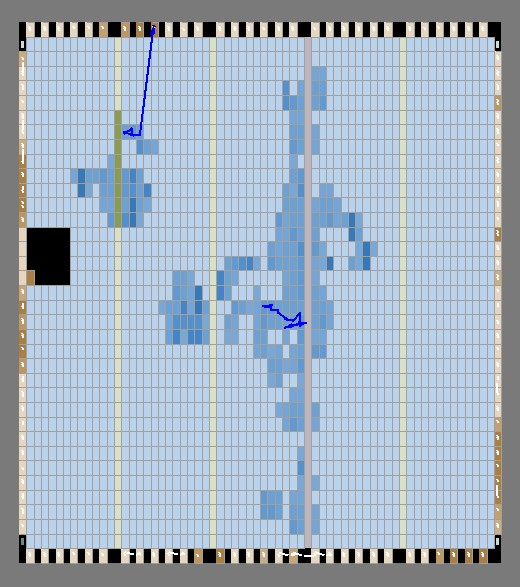
\includegraphics[width=0.5\textwidth]{img/Chip_planner_critical_path.jpg}
    \caption{Critical Path shown in the Chip Planner}
    \label{fig:Chip_planner_critical_path}
\end{figure}

\newpage
\paragraph{Fast model} \quad \\
The hold time slack for every clock source is shown in \autoref{fig:Hold_slack}

\begin{figure}[h!]
    \centering
    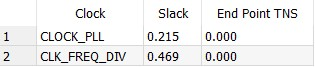
\includegraphics[width=0.5\textwidth]{img/Hold_slack.jpg}
    \caption{Hold time slack}
    \label{fig:Hold_slack}
\end{figure}

\noindent
To obtain this values of hold time slack we optimized all the path to increase the hold time slack. \\
To do this, we modified the Fitter settings as shown in \autoref{fig:fitter_settings}

\begin{figure}[h!]
    \centering
    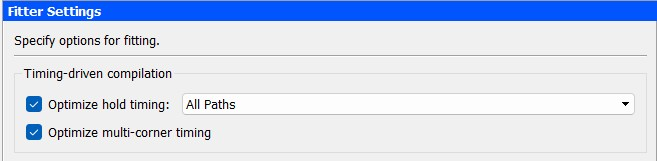
\includegraphics[width=0.8\textwidth]{img/fitter_settings.jpg}
    \caption{Fitter settings}
    \label{fig:fitter_settings}
\end{figure}

\subsection{Power consumption}
At the end of the Analysis and Synthesis, we run the Power Analyzer to check the power consumption of the project.\\
This analysis does not consider the power dissipated to drive the loads, because by default, the load capacitances are set to \(0\ \text{pF}\).\\
To perform a more accurate analysis, we have to estimate the load capacitance for each output of the circuit.

\vspace{0.5cm}
\begin{figure}[h!]
    \centering
    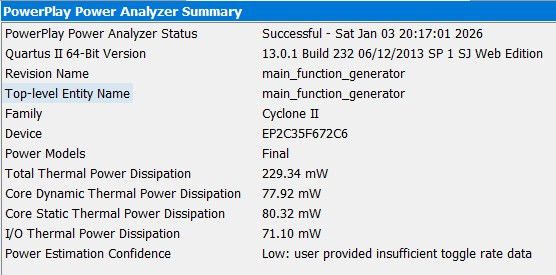
\includegraphics[width=0.6\textwidth]{img/power_analyzer_summary.jpg}
    \caption{Power analyzer summary}
    \label{fig:power_analyzer_summary}
\end{figure}

\noindent
The analyzer tool also allows you to see which parts of the power are dissipated and which portions are consumed by each block, as shown in
\autoref{fig:power_analyzer_summary_detailed}

\vspace{0.5cm}
\begin{figure}[h!]
    \centering
    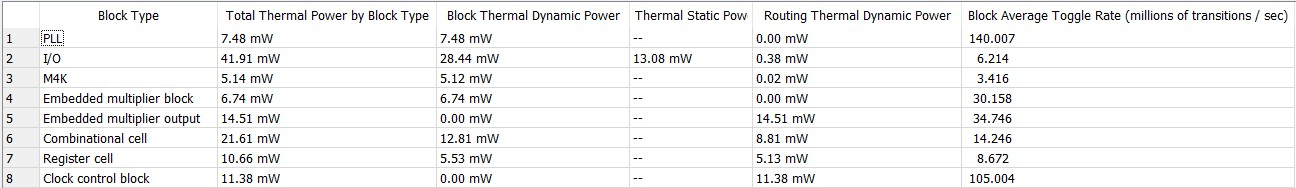
\includegraphics[width=1\textwidth]{img/power_analyzer_summary_detailed.jpg}
    \caption{Termal power dissipation by block type}
    \label{fig:power_analyzer_summary_detailed}
\end{figure}

\newpage

\subsection{Resource usage}
The internal FPGA resources used at the end of the Analysis and Synthesis operations are reported in \\ \autoref{fig:res_usage}.

\vspace{0.5cm}
\begin{figure}[h!]
    \centering
    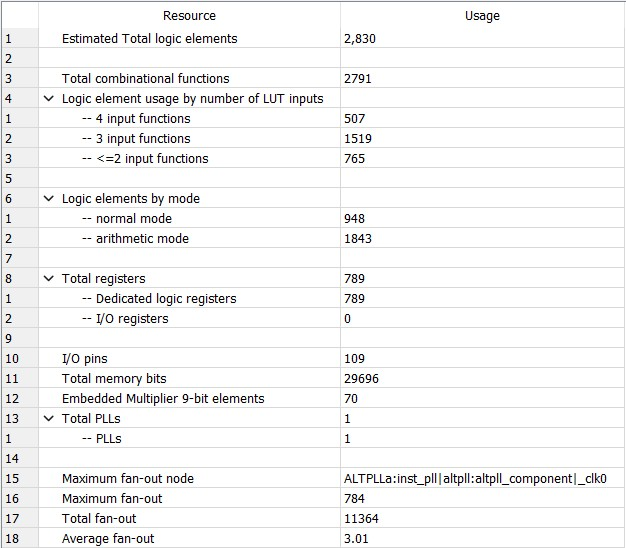
\includegraphics[width=0.8\textwidth]{img/resource usage.jpg}
    \caption{Resource usage table}
    \label{fig:res_usage}
\end{figure}
\vspace{0.5cm}

\noindent
Compared to all the resources available on the chip, the total logic elements used are only \(9\%\) of the total, and the total memory bits used are \(6\%\), as shown in \autoref{fig:flow_summary}. \\
Furthermore has been used all the embedded multiplier and one of the four internal PLL.

\vspace{0.5cm}
\begin{figure}[h!]
    \centering
    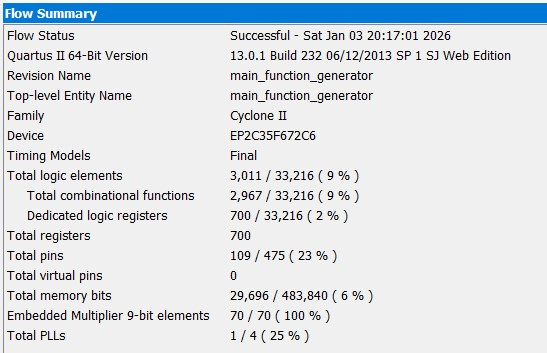
\includegraphics[width=0.8\textwidth]{img/flow_summary.jpg}
    \caption{Analysis and synthesis flow summary}
    \label{fig:flow_summary}
\end{figure}

\noindent
In the Chip Planner, we can see where are placed all the blocks of the project, inside the FPGA, as shown in \autoref{fig:chip_planner}

\vspace{0.5cm}
\begin{figure}[h!]
    \centering
    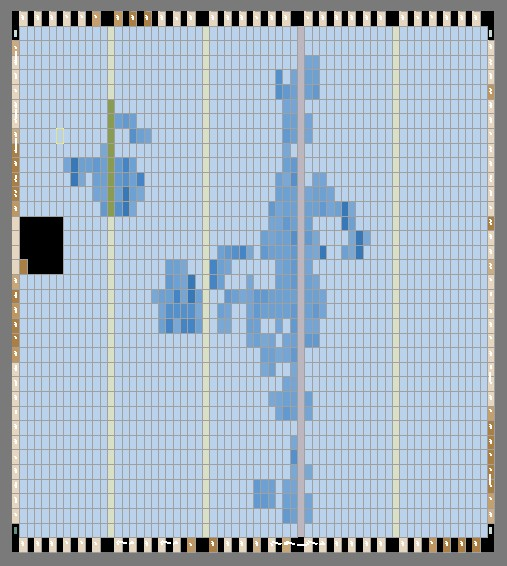
\includegraphics[width=0.8\textwidth]{img/chip_planner.jpg}
    \caption{Chip Planner}
    \label{fig:chip_planner}
\end{figure}
\vspace{0.5cm}


    \newpage
    \section{Conclusions}
\label{sec:conclusions}

We recall that the goal of the project was to design a function generator capable of producing output waveforms with frequencies up to \(1 MHz\). \\
Laboratory tests have shown that the proposed design fully meets the specified requirements. \\
Nevertheless, some parts of the system could be optimized, and several possible upgrades may be implemented to enhance the overall functionality of the design without significantly increasing the hardware complexity of the chip.

\subsection{Criticality}
Even though it has been verified with the timing analyzer that the dynamic clock generated by the frequency divider instantiated in the DDFS module does not cause any timing violations, this verification has been carried out by considering the clock source in phase with the main clock, without taking into account the \(t_{co}\) of the flip-flop. \\
To avoid potential issues, the divided clock can be considered asynchronous and the input can be protected using a flip-flop chain. \\
A more professional solution can be obtained by using a \texttt{clock\_enable} signal, which identifies, via a counter synchronized with the main clock, the \(n\)-th clock cycle and synchronizes the module using this signal, where \(n\) is controlled by the \texttt{freq\_control} input. \\
A possible Verilog implementation of the clock enable signal is shown in \autoref{lst:clk_ena}.

\vspace{0.5cm}
\begin{lstlisting}[language=Verilog, caption=Implementation of clock enable signal with frequency divider, 
label=lst:clk_ena ]
    integer cont;
    always @(posedge clk) begin
        if(rst_n == 0) begin
            //reset condition
            cont <= 0;
            clk_ena <= 1'b0;
        end
        else begin
            if(cont >= n) begin
                cont <= 0;
                clk_ena <= 1'b1;
            end
            else begin
                cont <= cont + 1;
                clk_ena <= 1'b0;
            end
        end
    end
\end{lstlisting}
\vspace{0.5cm}

\noindent
With the \texttt{clock\_ena} signal, all the sequential blocks synchronized with the divided frequency clock become like the block in \autoref{lst:clk_div_ena} 

\vspace{0.5cm}
\begin{lstlisting}[language=Verilog, caption=Avoid using divided clock, 
label=lst:clk_div_ena ]
    always @(posedge clk) begin
        if(clk_ena == 1) begin
            //divided clock operation
        end
        else begin
            //store the signals
        end
    end
\end{lstlisting}
\vspace{0.5cm}

\newpage

\subsection{Possible optimizations}
The first hardware optimization that can be done is inside the \texttt{DDFS\_frequency\_converter} where a large number of multipliers have been instantiated.

\vspace{0.5cm}
\begin{lstlisting}[language=Verilog, caption=Part of the calculations performed to obtain the frequency word value, 
label=lst:mult_inst_non_opt ]
    always @(*) begin
        
        if(final_freq <= (CLK_FREQ/(1000000*MIN_LUT_SAMPLE))) begin
            freq_control = 3'd6;
            fw = (fw_1000000 >= 0) ? fw_1000000 : 7'd0;
        end 
        else if(final_freq <= (CLK_FREQ/(100000*MIN_LUT_SAMPLE))) begin
            freq_control = 3'd5;
            fw = (fw_100000 >= 0) ? fw_100000 : 7'd0;
        end
        .
        .
        .
        
        else begin
            //default condition, max frequency
            freq_control = 3'd0;
            fw = 7'd0;
        end
        
    end

    always @(posedge clk) begin
        ...
    
        fw_1000000 <= (mult_1000000*K)>>54;
        fw_100000 <= (mult_100000*K)>>54;
        fw_10000 <= (mult_10000*K)>>54;
        fw_1000 <= (mult_1000*K)>>54;
        fw_100 <= (mult_100*K)>>54;
        fw_10 <= (mult_10*K)>>54;
        fw_2 <= (mult_2*K)>>54;
    end
\end{lstlisting}
\vspace{0.5cm}

\noindent
In \autoref{lst:mult_inst_non_opt}, is calculated the value of \texttt{f\_w} for every clock value that goes into the DDFS module. \\
\texttt{fw\_2} is the frequency word calculated with the clock divided by two, \texttt{fw\_10} is the same with the clock divided by ten and so on.

\newpage
\noindent
The problem is that \texttt{mult\_*} is a \(64 bit\) value, so the multipliers instantiated are big combinatorial network. \\
To reduce the number of multiplier instantiated the input of the operation can be multiplexed as shown in \autoref{lst:mult_inst_opt}

\vspace{0.5cm}
\begin{lstlisting}[language=Verilog, caption=Example to optimize the calculation of frequency word value, 
label=lst:mult_inst_opt ]
    always (*) begin
    
        if(final_freq <= (CLK_FREQ/(1000000*MIN_LUT_SAMPLE))) begin
            freq_control = 3'd6;
            mult = mult_1000000;
        end 
        else if(final_freq <= (CLK_FREQ/(100000*MIN_LUT_SAMPLE))) begin
            freq_control = 3'd5;
            mult = mult_100000;
        end
        .
        .
        .
        
        else begin
            //default condition, max frequency
            freq_control = 3'd0;
            mult = mult_2;
        end

    end

    always (posedge clk) begin
        ...
        
        fw <= (mult*K)>>54;
    end
\end{lstlisting}
\vspace{0.5cm}

\noindent
This optimization instantiates a multiplexer and can reduce the maximum frequency of the project; to overcome this problem, the multiplexing operation can be pipelined by modifying the combinatorial block into a synchronous block. \\
The pipeline operation increases the frequency but also the throughput of the system.\\
Another optimization that can be done is to allow the \texttt{ddfs} module to work with its own clock source and control it asynchronously using a FIFO memory.\\
This is because the \texttt{ddfs} module can work at a frequency much higher than the other modules, due to its hardware simplicity, and the other modules are used to interface with the operator, so they can produce the outputs even after some milliseconds.\\
This upgrade allows the frequency generator to produce higher-frequency waveforms without increasing the complexity of the circuit. \\
Another possible optimization concerns the LUTs that store the contents of the screens displayed on the LCD. For future upgrades, some spaces are left blank to allow the addition of more pages. However, in the final version, all unused blank spaces can be removed, reducing the amount of instantiated LUT memory.

\subsection{Possible upgrades}
A simple upgrade that can be made is to instantiate two additional \texttt{ddfs} modules within the project and assign each module a dedicated button on the keypad. \\
By doing this, we can use all three DAC outputs to generate dedicated waveforms. \\
A more advanced update could also allow the modules to communicate with each other, enabling their outputs to be synchronized, either in phase or with a programmed phase shift. \\
Furthermore, it is possible to implement a method, via USB communication or SD card, to upload samples of customizable waveforms for display. These samples are then saved into the board's internal FLASH memory and can be displayed when needed. \\
Before displaying a custom waveform, it is important to transfer the samples from FLASH to internal RAM, since the read latency of FLASH significantly reduces the output frequency of the waveform.
    
    
\end{document}

